% 
%            ,,                                        
%          `7MM            _.o9                                
%            MM                                             
%  ,6"Yb.    MM  ,p6"bo   ,6"Yb.  M"""MMV  ,6"Yb.  `7Mb,od8 
% 8)   MM    MM 6M'  OO  8)   MM  '  AMV  8)   MM    MM' "' 
%  ,pm9MM    MM 8M        ,pm9MM    AMV    ,pm9MM    MM     
% 8M   MM    MM YM.    , 8M   MM   AMV  , 8M   MM    MM     
% `Moo9^Yo..JMML.YMbmd'  `Moo9^Yo.AMMmmmM `Moo9^Yo..JMML.   
% 
% 
% Free, Open-Source Thesis template for LaTeX
% https://github.com/dpmj/alcazar


% %%%%%%%%%%%%%%%%%%%%%%%%%%%%%%%%%%%%%%%%%%%%%%%%%%%%%%%%%%%%%%%%%%%%%%%%%%%%%%
% PREAMBLE

\documentclass[twoside, openright, 11pt]{report}


% ------------------------------------------------------------------------------
% Variables

% Title for the title page 
\newcommand{\thesisTitle}{Optimizing convolutional architectures for geospatial analysis in global earth system models}
% Title for the pages' heading 
\newcommand{\thesisTitleShort}{Optimizing convolutional architectures for geospatial analysis in global earth system models}

\newcommand{\thesisType}{Master's Thesis}  % Bachelor's Thesis, Master's Thesis, PhD Thesis...
\newcommand{\thesisDegree}{Master's Degree}  % Bachelor's Degree, Master's Degree, PhD...

\newcommand{\thesisAuthor}{Syed Usman Farooq}
\newcommand{\thesisTutor}{Msc. Yannick Wölker}  

\newcommand{\thesisYear}{2077}  % Date of the thesis' submission or defense 
\newcommand{\thesisMonth}{June}
\newcommand{\thesisDate}{{\thesisMonth} {\thesisYear}}
\newcommand{\thesisAcademicCourse}{2076/2077}  % During which academic year(s) was the thesis developed

\newcommand{\thesisSchool}{Universitat Politècnica de València}
\newcommand{\thesisAddress}{Camí de Vera, s/n, 46022 València, Valencia, Spain}
\newcommand{\thesisDepartment}{Department of Electronic Engineering}

\newcommand{\thesisKeywords}{Keyword 1, Keyword 2, Keyword 3, Keyword 4, Keyword 4, Keyword 5, Keyword 6, Keyword 7, Keyword 8, Keyword 9, Keyword 10, Keyword N}  
% For the abstract and indexing


% ------------------------------------------------------------------------------
% Import document style
\usepackage{style/alcazar}
\usepackage{amsfonts}
\usepackage{hyperref}


% END PREAMBLE
% %%%%%%%%%%%%%%%%%%%%%%%%%%%%%%%%%%%%%%%%%%%%%%%%%%%%%%%%%%%%%%%%%%%%%%%%%%%%%%
% BEGIN DOCUMENT

\begin{document}

% Titlepage, license, about, abstract, keywords, publications, acknowledgements, dedication and tables of contents
% 
%            ,,                                        
%          `7MM            _.o9                                
%            MM                                             
%  ,6"Yb.    MM  ,p6"bo   ,6"Yb.  M"""MMV  ,6"Yb.  `7Mb,od8 
% 8)   MM    MM 6M'  OO  8)   MM  '  AMV  8)   MM    MM' "' 
%  ,pm9MM    MM 8M        ,pm9MM    AMV    ,pm9MM    MM     
% 8M   MM    MM YM.    , 8M   MM   AMV  , 8M   MM    MM     
% `Moo9^Yo..JMML.YMbmd'  `Moo9^Yo.AMMmmmM `Moo9^Yo..JMML.   
% 
% 
% Free and Open-Source template for academic works
% https://github.com/dpmj/alcazar



% ------------------------------------------------------------------------------
% FILES

% Title page
% 
%            ,,                                        
%          `7MM            _.o9                                
%            MM                                             
%  ,6"Yb.    MM  ,p6"bo   ,6"Yb.  M"""MMV  ,6"Yb.  `7Mb,od8 
% 8)   MM    MM 6M'  OO  8)   MM  '  AMV  8)   MM    MM' "' 
%  ,pm9MM    MM 8M        ,pm9MM    AMV    ,pm9MM    MM     
% 8M   MM    MM YM.    , 8M   MM   AMV  , 8M   MM    MM     
% `Moo9^Yo..JMML.YMbmd'  `Moo9^Yo.AMMmmmM `Moo9^Yo..JMML.   
% 
% 
% Free and Open-Source template for academic works
% https://github.com/dpmj/alcazar


% ------------------------------------------------------------------------------
% Title page

\thispagestyle{empty}

\pagenumbering{roman}
\setcounter{page}{1}


\newgeometry{
    left    = 3.0cm,
    right   = 3.0cm,
    top     = 3.5cm,
    bottom  = 3.5cm
}


\begin{center}
    
\includegraphics[height=15mm]{opening/resources/logos/logo_upv.pdf}
    \hfill
    
\includegraphics[height=15mm]{opening/resources/logos/logo_upv_telcom.pdf}
\end{center}

\vspace*{30mm}

\begin{center}
    \textbf{\large \textsc{{\thesisDegree} in}}
\end{center}

\vspace*{0mm}

\begin{center}
    \textbf{\large \thesisType}
\end{center}

\vspace*{10mm}

\begin{center}
    \setstretch{1.7}
    \textbf{{\LARGE {}``\thesisTitle''}}\\
\end{center}

\vspace*{15mm}

\begin{center}
    {\large \textsc{Academic course:} \thesisAcademicCourse}
\end{center}

\vspace*{15mm}

\begin{center}
    AUTHOR:
    \par
    \textbf{{\large \thesisAuthor}}
\end{center}

\begin{center}
    TUTOR:
    \par
    \textbf{{\large \thesisTutor}}
\end{center}

\begin{center}
    \vspace*{1mm}
    {\large \thesisDepartment}
\end{center}

\newpage
\thispagestyle{empty}
\restoregeometry


% License
% % 
%            ,,                                        
%          `7MM            _.o9                                
%            MM                                             
%  ,6"Yb.    MM  ,p6"bo   ,6"Yb.  M"""MMV  ,6"Yb.  `7Mb,od8 
% 8)   MM    MM 6M'  OO  8)   MM  '  AMV  8)   MM    MM' "' 
%  ,pm9MM    MM 8M        ,pm9MM    AMV    ,pm9MM    MM     
% 8M   MM    MM YM.    , 8M   MM   AMV  , 8M   MM    MM     
% `Moo9^Yo..JMML.YMbmd'  `Moo9^Yo.AMMmmmM `Moo9^Yo..JMML.   
% 
% 
% Free and Open-Source template for academic works
% https://github.com/dpmj/alcazar


%%%%%%%%%%%%%%%%%%%%%%%%%%%%%%%%%%%%%%%%%%%%%%%%%%%%%%%%%%%%%%%%%%%%%%%%%%%%%%%%%%%%%%%%%%%%
% LICENSE

\newpage
\thispagestyle{empty}

\vspace*{\fill}

\begingroup

    \setlength\tabcolsep{0pt}
    \renewcommand*{\arraystretch}{1.4}
    \renewcommand{\baselinestretch}{0.9}\footnotesize  % Comprime space
    
    \noindent
    \begin{tabular}{m{3.5cm} m{11.5cm}}
        
\includegraphics[width=3cm]{opening/resources/license/by-sa.pdf} & {\normalsize {\thesisAuthor} and {\thesisTutor}} \\
    \end{tabular}
    
    \noindent This work is licensed under the Creative Commons Attribution-ShareAlike 4.0 International (CC BY-SA 4.0) license. This is a human-readable summary of (and not a substitute for) the license. You are free to:
    
    \noindent
    \begin{tabular}{m{1.5cm} m{13.5cm}}
        \textbf{Share} & Copy and redistribute the material in any medium or format.\\
        \textbf{Adapt} & Remix, transform, and build upon the material.\\
    \end{tabular}
    
    \vspace{1mm}
    
    \noindent The licensor cannot revoke these freedoms as long as you follow the license terms:
    
    \noindent
    \begin{tabular}{m{1.5cm} m{13.5cm}}
        
\includegraphics[width=2em]{opening/resources/license/by.pdf} & \textbf{Attribution:} You must give appropriate credit, provide a link to the license, and indicate if changes were made. You may do so in any reasonable manner, but not in any way that suggests the licensor endorses you or your use.\\
        
\includegraphics[width=2em]{opening/resources/license/sa.pdf} & \textbf{ShareAlike:} If you remix, transform, or build upon the material, you must distribute your contributions under the same license as the original.
    \end{tabular}
    
    \noindent To view a complete copy of this license, visit 
    \href{https://creativecommons.org/licenses/by-nc-sa/4.0/}{https://creativecommons.org/licenses/by-sa/4.0}

\endgroup


% Give a little credit to the template :)
% It's completely optional, of course ;)

\begingroup

    \vspace*{2mm}

    \setlength\tabcolsep{0pt}
    \renewcommand*{\arraystretch}{1.4}
    \renewcommand{\baselinestretch}{0.9}\footnotesize  % Comprime space
    
    \noindent
    \begin{tabular}{m{3.5cm} m{11.5cm}}
        
\includegraphics[width=3cm]{opening/resources/logos/alcazar.pdf} & \noindent This document has been generated using {\href{https://github.com/dpmj/alcazar}{Alcázar}}, a free and open source {\LaTeX} template for academic works by \href{https://www.linkedin.com/in/dpmj/}{Juan Del Pino Mena}. \\
    \end{tabular}

    

\endgroup




% About the document
% Collaborators, repositories, social networks, links, etc.
% Feel free to edit this doc:
% % 
%            ,,                                        
%          `7MM            _.o9                                
%            MM                                             
%  ,6"Yb.    MM  ,p6"bo   ,6"Yb.  M"""MMV  ,6"Yb.  `7Mb,od8 
% 8)   MM    MM 6M'  OO  8)   MM  '  AMV  8)   MM    MM' "' 
%  ,pm9MM    MM 8M        ,pm9MM    AMV    ,pm9MM    MM     
% 8M   MM    MM YM.    , 8M   MM   AMV  , 8M   MM    MM     
% `Moo9^Yo..JMML.YMbmd'  `Moo9^Yo.AMMmmmM `Moo9^Yo..JMML.   
% 
% 
% Free and Open-Source template for academic works
% https://github.com/dpmj/alcazar

\newpage


\clearpage
\cleardoublepage
\phantomsection

\pagestyle{empty}

\phantomsection
\addcontentsline{toc}{chapter}{About this work}


%%%%%%%%%%%%%%%%%%%%%%%%%%%%%%%%%%%%%%%%%%%%%%%%%%%%%%%%%%%%%%%%%%%%%%%%%%%%%%%%%%%%%%%%%%%%
% ABOUT THE AUTHORS

\begingroup

    \small
    \setlength\tabcolsep{0pt}
    \renewcommand*{\arraystretch}{1}
    
    \noindent
    \begin{tabular}{p{3.5cm} p{11.5cm}}
        \vspace{0mm} 
\includegraphics[width=3cm]{opening/resources/about/kleiner.png} & \vspace{-0.5mm} {\large \thesisAuthor} 
        \newline A short paragraph about you and how handsome and hard-working you are. Brag about your work, awards, publications and merits. The glory is yours! Congratulations. The Lorem ipsum dolor sit amet, consectetur adipiscing elit. Integer tempus quis elit id sagittis. Cras tincidunt nisi at tellus luctus, et congue dolor posuere. Aliquam suscipit felis sit amet lacus ultrices aliquet. Sed sagittis ultrices nisi, vel elementum elit dignissim non. 
        \vspace{2mm} 
        \newline
        \href{https://orcid.org/}{  % Link to your orcid
            \icon{\faOrcid}{10}{orcid-green}
        }
        \href{https://www.linkedin.com/}{  % Link to your linkedin
            \icon{\faLinkedinIn}{10}{linkedin-blue}
        }
        \href{https://github.com/}{  % Link to your github
            \icon{\faGithub}{10}{github-black}
        }
        \href{https://twitter.com/}{  % Link to your twitter
            \icon{\faTwitter}{10}{twitter-blue}
        }
        \href{mailto:example@domain.org}{  % Your E-mail
            \icon{\faEnvelope}{10}{email-red}
        }
        \href{https://t.me/}{  % Link to your telegram
            \icon{\faTelegramPlane}{10}{telegram-blue}
        }
    \end{tabular}
    
    \vspace{10mm}
    
    \noindent
    \begin{tabular}{p{3.5cm} p{11.5cm}}
        \vspace{0mm} 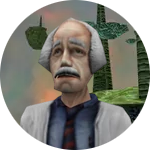
\includegraphics[width=3cm]{opening/resources/about/coomer.png} & \vspace{-0.5mm} {\large \thesisTutor} 
        \newline What a big fish you've got yourself. Show off your tutor. Now that's a job well done. Lorem ipsum dolor sit amet, consectetur adipiscing elit. Integer tempus quis elit id sagittis. Cras tincidunt nisi at tellus luctus, et congue dolor posuere. Aliquam suscipit felis sit amet lacus ultrices aliquet. Sed sagittis ultrices nisi, vel elementum elit dignissim non. Fusce faucibus ex at massa ultrices elementum.
        \vspace{2mm} 
        \newline
        \href{https://orcid.org/}{  % Link to your orcid
            \icon{\faOrcid}{10}{orcid-green}
        }
        \href{https://www.linkedin.com/}{  % Link to your linkedin
            \icon{\faLinkedinIn}{10}{linkedin-blue}
        }
        \href{https://github.com/}{  % Link to your github
            \icon{\faGithub}{10}{github-black}
        }
        \href{https://twitter.com/}{  % Link to your twitter
            \icon{\faTwitter}{10}{twitter-blue}
        }
        \href{mailto:example@domain.org}{  % Your E-mail
            \icon{\faEnvelope}{10}{email-red}
        }
        \href{https://t.me/}{  % Link to your telegram
            \icon{\faTelegramPlane}{10}{telegram-blue}
        }
    \end{tabular}
    
\endgroup





%%%%%%%%%%%%%%%%%%%%%%%%%%%%%%%%%%%%%%%%%%%%%%%%%%%%%%%%%%%%%%%%%%%%%%%%%%%%%%%%%%%%%%%%%%%%
% how to cite this work

% Listings workaround to include the background in broken lines

% \begin{verbatimwrite}{cite.txt}
% @mastersthesis{citeKey,
%     author  = "(*@{\thesisAuthor}@*) and (*@{\thesisTutor}@*)",
%     title   = "(*@{\thesisTitle}@*)",
%     school  = "(*@{\thesisSchool}@*)",
%     year    = "(*@{\thesisYear}@*)",
%     month   = "(*@{\thesisMonth}@*)",
%     address = "(*@{\thesisAddress}@*)"
% }
% \end{verbatimwrite}


\begingroup

\vspace*{\fill}

\small
\setlength\tabcolsep{0pt}
\renewcommand*{\arraystretch}{1.2}
{\noindent\large  Cite this work:}

% \begin{mdframed}[backgroundcolor=listing-background,hidealllines=true]
\vspace*{2mm}
% \lstinputlisting[style=cite, nolol]{./cite.txt}

\newwrite\tempfile
\immediate\openout\tempfile=cite.txt
\immediate\write\tempfile{%
@mastersthesis{citeKey,^^J
author  = "\thesisAuthor \space and \thesisTutor",^^J
title   = "\thesisTitle",^^J
school  = "\thesisSchool",^^J
year    = "\thesisYear",^^J
month   = "\thesisMonth",^^J
address = "\thesisAddress",^^J
type = "\thesisType"^^J
}
}
\immediate\closeout\tempfile

% Does not work because escapes are inside strings
% \begin{minted}{bibtex}
% @mastersthesis{citeKey,
%     author  = "¢{\thesisAuthor}¢ and ¢{\thesisTutor}¢",
%     title   = "¢{\thesisTitle}¢",
%     school  = "¢{\thesisSchool}¢",
%     year    = "¢{\thesisYear}¢",
%     month   = "¢{\thesisMonth}¢",
%     address = "¢{\thesisAddress}¢"
% }
% \end{minted}

\inputminted[style=algol_nu]{bibtex}{./cite.txt}
% \end{mdframed}


\endgroup

\newpage
\thispagestyle{empty}


\cleardoublepage
\phantomsection
\begin{center}
    \textbf{\large DECLARATION}
\end{center}


I declare that have produced the Master’s thesis \textbf{\thesisTitle} independently and without improper external assistance and that I have identified all
word-for-word quotations of other authors, as well as comments based closely on other authors’ ideas, and I have listed the relevant sources.


I am aware that, unless agreed otherwise, the Master’s thesis  produced under supervision represents a group achievement and forms part of the overall
research of the supervising institution. As a result, none of the co-authors (e.g. authors of text, creative project staff, co-supervisors) may use passages
from the thesis for commercial purposes or make them accessible to third parties without the (written) approval of all those involved due to reasons of copyright.
Particular note must be taken of the Arbeitnehmererfindergesetz (German Employee Invention Act), according to which pre-publication of patent-related content is prohibited.




\vspace*{2cm}
\noindent
\begin{minipage}[t]{0.5\textwidth}
    \textbf{Date:} \today
\end{minipage}%
\begin{minipage}[t]{0.5\textwidth}
    \flushright
    \textbf{Signature:} \underline{\hspace{4cm}}
\end{minipage}

% Abstract
% 
%            ,,                                        
%          `7MM            _.o9                                
%            MM                                             
%  ,6"Yb.    MM  ,p6"bo   ,6"Yb.  M"""MMV  ,6"Yb.  `7Mb,od8 
% 8)   MM    MM 6M'  OO  8)   MM  '  AMV  8)   MM    MM' "' 
%  ,pm9MM    MM 8M        ,pm9MM    AMV    ,pm9MM    MM     
% 8M   MM    MM YM.    , 8M   MM   AMV  , 8M   MM    MM     
% `Moo9^Yo..JMML.YMbmd'  `Moo9^Yo.AMMmmmM `Moo9^Yo..JMML.   
% 
% 
% Free and Open-Source template for academic works
% https://github.com/dpmj/alcazar

\newpage

\clearpage
\cleardoublepage
\phantomsection

\pagestyle{plain}

\phantomsection
\addcontentsline{toc}{chapter}{Abstract}

{\noindent \large \textbf{\thesisTitle}}\\

{\noindent \textbf{\textsc{Keywords:}}}

{\noindent \thesisKeywords}\\


{\noindent \textbf{\textsc{Abstract:}}}

\noindent Abstract in the same language as the main text. Lorem ipsum dolor sit amet, consectetur adipiscing elit. Integer tempus quis elit id sagittis. Cras tincidunt nisi at tellus luctus, et congue dolor posuere. Aliquam suscipit felis sit amet lacus ultrices aliquet. Sed sagittis ultrices nisi, vel elementum elit dignissim non. Fusce faucibus ex at massa ultrices elementum. Nullam ullamcorper lorem sit amet facilisis cursus. Suspendisse non erat non justo porta placerat. Morbi porttitor dictum molestie. Sed vitae iaculis libero. Suspendisse in gravida lacus, tempor ultrices nibh. Nam consequat scelerisque porttitor.

Nulla elementum orci in dolor dapibus, ac facilisis sem ultrices. Nullam eleifend id eros sed luctus. Maecenas arcu ipsum, scelerisque id lorem in, placerat posuere tellus. Etiam gravida velit sed arcu viverra dapibus. Mauris vitae augue dapibus, molestie justo eget, condimentum ipsum. Nulla tristique mi eget semper luctus. Etiam commodo vestibulum vulputate. Etiam quis sapien dolor. Nunc tristique eu lacus quis ullamcorper. Sed volutpat rutrum vehicula. Donec nunc nisl, suscipit in faucibus vitae, tristique eu risus. Nulla facilisis augue eget interdum rutrum. Aliquam sem nunc, fermentum sed urna ac, faucibus interdum nisi.

Proin a condimentum nibh. Praesent vulputate tellus vel metus rutrum, non luctus mi sollicitudin. Nam ac tellus ut eros sollicitudin luctus at ac mi. Vestibulum mollis nec nisi a laoreet. Proin neque tortor, placerat nec suscipit sit amet, ullamcorper in sem. Fusce faucibus ultrices cursus. Maecenas scelerisque mauris diam, at volutpat nisi porta vitae. Sed at ipsum et leo cursus varius eu eu lectus. Class aptent taciti sociosqu ad litora torquent per conubia nostra, per inceptos himenaeos. Ut felis ipsum, imperdiet rhoncus orci ac, consectetur luctus nisl. Cras aliquet elementum tellus ullamcorper malesuada. Integer purus est, pharetra eu ullamcorper quis, imperdiet non turpis.

In vestibulum faucibus ligula eget blandit. Donec eget cursus risus, quis suscipit justo. Curabitur efficitur, dolor nec pulvinar pellentesque, lectus eros hendrerit nisi, in aliquet erat nunc non ipsum. Curabitur felis nunc, viverra nec quam ultrices, suscipit condimentum nibh. Nam faucibus felis hendrerit imperdiet maximus. Curabitur tincidunt porttitor lectus quis feugiat. Sed imperdiet bibendum mi.

Nullam quis lacus vel ante feugiat efficitur id ut quam. Pellentesque commodo elit nec urna gravida maximus. Suspendisse ut risus eu ipsum porta porta ac et orci. Donec dictum ligula sodales, euismod est sed, semper libero. In blandit, nulla et elementum pharetra, mi nunc sagittis tellus, sit amet scelerisque magna elit ac sapien. Curabitur ipsum dui, pretium a maximus id, varius gravida nisl. Sed vitae mattis elit, vitae hendrerit lorem. 



%% ADDITIONAL LANGUAGES
% Translate your title and keywords to match the language


\newpage
\thispagestyle{empty}

\clearpage
\cleardoublepage
\phantomsection

\pagestyle{plain}

{\noindent \large \textbf{\thesisTitle}}\\

{\noindent \textbf{\textsc{Palabras clave:}}}

{\noindent \thesisKeywords}\\


{\noindent \textbf{\textsc{Resumen:}}}

\noindent Resumen en un idioma diferente - Abstract in a different language.
Lorem ipsum dolor sit amet, consectetur adipiscing elit. Integer tempus quis elit id sagittis. Cras tincidunt nisi at tellus luctus, et congue dolor posuere. Aliquam suscipit felis sit amet lacus ultrices aliquet. Sed sagittis ultrices nisi, vel elementum elit dignissim non. Fusce faucibus ex at massa ultrices elementum. Nullam ullamcorper lorem sit amet facilisis cursus. Suspendisse non erat non justo porta placerat. Morbi porttitor dictum molestie. Sed vitae iaculis libero. Suspendisse in gravida lacus, tempor ultrices nibh. Nam consequat scelerisque porttitor.

Nulla elementum orci in dolor dapibus, ac facilisis sem ultrices. Nullam eleifend id eros sed luctus. Maecenas arcu ipsum, scelerisque id lorem in, placerat posuere tellus. Etiam gravida velit sed arcu viverra dapibus. Mauris vitae augue dapibus, molestie justo eget, condimentum ipsum. Nulla tristique mi eget semper luctus. Etiam commodo vestibulum vulputate. Etiam quis sapien dolor. Nunc tristique eu lacus quis ullamcorper. Sed volutpat rutrum vehicula. Donec nunc nisl, suscipit in faucibus vitae, tristique eu risus. Nulla facilisis augue eget interdum rutrum. Aliquam sem nunc, fermentum sed urna ac, faucibus interdum nisi.

Proin a condimentum nibh. Praesent vulputate tellus vel metus rutrum, non luctus mi sollicitudin. Nam ac tellus ut eros sollicitudin luctus at ac mi. Vestibulum mollis nec nisi a laoreet. Proin neque tortor, placerat nec suscipit sit amet, ullamcorper in sem. Fusce faucibus ultrices cursus. Maecenas scelerisque mauris diam, at volutpat nisi porta vitae. Sed at ipsum et leo cursus varius eu eu lectus. Class aptent taciti sociosqu ad litora torquent per conubia nostra, per inceptos himenaeos. Ut felis ipsum, imperdiet rhoncus orci ac, consectetur luctus nisl. Cras aliquet elementum tellus ullamcorper malesuada. Integer purus est, pharetra eu ullamcorper quis, imperdiet non turpis.

In vestibulum faucibus ligula eget blandit. Donec eget cursus risus, quis suscipit justo. Curabitur efficitur, dolor nec pulvinar pellentesque, lectus eros hendrerit nisi, in aliquet erat nunc non ipsum. Curabitur felis nunc, viverra nec quam ultrices, suscipit condimentum nibh. Nam faucibus felis hendrerit imperdiet maximus. Curabitur tincidunt porttitor lectus quis feugiat. Sed imperdiet bibendum mi.

Nullam quis lacus vel ante feugiat efficitur id ut quam. Pellentesque commodo elit nec urna gravida maximus. Suspendisse ut risus eu ipsum porta porta ac et orci. Donec dictum ligula sodales, euismod est sed, semper libero. In blandit, nulla et elementum pharetra, mi nunc sagittis tellus, sit amet scelerisque magna elit ac sapien. Curabitur ipsum dui, pretium a maximus id, varius gravida nisl. Sed vitae mattis elit, vitae hendrerit lorem. 




% Publications
% 
%            ,,                                        
%          `7MM            _.o9                                
%            MM                                             
%  ,6"Yb.    MM  ,p6"bo   ,6"Yb.  M"""MMV  ,6"Yb.  `7Mb,od8 
% 8)   MM    MM 6M'  OO  8)   MM  '  AMV  8)   MM    MM' "' 
%  ,pm9MM    MM 8M        ,pm9MM    AMV    ,pm9MM    MM     
% 8M   MM    MM YM.    , 8M   MM   AMV  , 8M   MM    MM     
% `Moo9^Yo..JMML.YMbmd'  `Moo9^Yo.AMMmmmM `Moo9^Yo..JMML.   
% 
% 
% Free and Open-Source template for academic works
% https://github.com/dpmj/alcazar


% Add here your Publications.
% Depends on Biblatex and Biber for multiple bibliographies.

\newpage
\pagestyle{empty}

\clearpage
\cleardoublepage
\phantomsection

\pagestyle{empty}

% \phantomsection
% \addcontentsline{toc}{chapter}{Publications}


\begin{refsection}

    \nocite{own-article-1, own-article-2, own-article-3}

    \defbibnote{pre-note}{
        \noindent The {\thesisDegree} candidate, {\thesisAuthor}, has co-authored the following publications with Prof. {\thesisTutor} et al. The articles come as a result of the research activities carried out during the {\thesisType}. The candidate is the corresponding author in two of the three publications listed below:
    }
    \defbibnote{post-note}{
        \noindent Note: \cite{own-article-3} is not yet published.
    }

    \printbibliography[heading=bibintoc,  % Title in Table of contents
                       title={Publications},  % Title
                       prenote=pre-note,  % Text before bibliography
                       postnote=post-note]  % Text after bibliography

\end{refsection}


  % Optional: comment this line if you don't need it

% Acknowledgements
% % 
%            ,,                                        
%          `7MM            _.o9                                
%            MM                                             
%  ,6"Yb.    MM  ,p6"bo   ,6"Yb.  M"""MMV  ,6"Yb.  `7Mb,od8 
% 8)   MM    MM 6M'  OO  8)   MM  '  AMV  8)   MM    MM' "' 
%  ,pm9MM    MM 8M        ,pm9MM    AMV    ,pm9MM    MM     
% 8M   MM    MM YM.    , 8M   MM   AMV  , 8M   MM    MM     
% `Moo9^Yo..JMML.YMbmd'  `Moo9^Yo.AMMmmmM `Moo9^Yo..JMML.   
% 
% 
% Free and Open-Source template for academic works
% https://github.com/dpmj/alcazar


% Add here your Acknowledgements. 
% This section is pretty free: free format, in one or various languages, etc.


\newpage
\thispagestyle{empty}

\clearpage
\cleardoublepage
\phantomsection

\pagestyle{plain}

\phantomsection
\addcontentsline{toc}{chapter}{Acknowledgements}


\vspace*{\fill}

\begin{center}
    \large \textbf{\textsc{Acknowledgements}}
\end{center}

@TODO start from here [usman]



% Dedication
% To whom do you dedicate the thesis? Or maybe include a quote, poem, etc. Free space for yourself.
% Delete if you are too manly for these things
% % 
%            ,,                                        
%          `7MM            _.o9                                
%            MM                                             
%  ,6"Yb.    MM  ,p6"bo   ,6"Yb.  M"""MMV  ,6"Yb.  `7Mb,od8 
% 8)   MM    MM 6M'  OO  8)   MM  '  AMV  8)   MM    MM' "' 
%  ,pm9MM    MM 8M        ,pm9MM    AMV    ,pm9MM    MM     
% 8M   MM    MM YM.    , 8M   MM   AMV  , 8M   MM    MM     
% `Moo9^Yo..JMML.YMbmd'  `Moo9^Yo.AMMmmmM `Moo9^Yo..JMML.   
% 
% 
% Free and Open-Source template for academic works
% https://github.com/dpmj/alcazar

\newpage
\thispagestyle{empty}

\clearpage
\cleardoublepage
\phantomsection

\thispagestyle{empty}

\phantomsection
\addcontentsline{toc}{chapter}{Dedication}



\vspace*{\fill}

\begin{flushright}

\textit{\large
\noindent ``Y así, mi señor, es como sabemos que\\
la Tierra tiene forma de plátano''\\ 
}

\vspace{0.5cm}

\textbf{Sir Bedevere el Sabio}\\

\vspace{0.3cm}

Interpretado por \textsc{Terry Jones}\\

\vspace{0.2cm}

{
\noindent En \textit{Monty Python y los caballeros\\
de la mesa cuadrada,} 1975\\
}

\vspace{2cm}
\end{flushright}



\vspace*{\fill}



% ------------------------------------------------------------------------------
% TABLES OF CONTENTS

\newpage
\thispagestyle{empty}

\clearpage
\cleardoublepage
\phantomsection

\pagestyle{plain}


\begingroup

% Greatly compress space used by TOC, LOF and LOT
\renewcommand{\baselinestretch}{1}  % less spacing
\small  % smaller font size
\setlength{\parskip}{0mm}  % Paragraph skip 0mm


% List of Contents
{
    \tableofcontents

    \addcontentsline{toc}{chapter}{Table of contents}
}

% List of Figures
{
    \listoffigures
    \addcontentsline{toc}{chapter}{List of figures}
}

% List of Tables
{
    \listoftables
    \addcontentsline{toc}{chapter}{List of tables}
}

% List of Listings -- uncomment if necessary
{
    % \listoflistings
    % \addcontentsline{toc}{chapter}{List of listings}

    % \listof{lstlisting}{Code listings} % old code
}

\endgroup

% END OPENING
% ------------------------------------------------------------------------------




% Glossary and acronyms
% 
%            ,,                                        
%          `7MM            _.o9                                
%            MM                                             
%  ,6"Yb.    MM  ,p6"bo   ,6"Yb.  M"""MMV  ,6"Yb.  `7Mb,od8 
% 8)   MM    MM 6M'  OO  8)   MM  '  AMV  8)   MM    MM' "' 
%  ,pm9MM    MM 8M        ,pm9MM    AMV    ,pm9MM    MM     
% 8M   MM    MM YM.    , 8M   MM   AMV  , 8M   MM    MM     
% `Moo9^Yo..JMML.YMbmd'  `Moo9^Yo.AMMmmmM `Moo9^Yo..JMML.   
% 
% 
% Free and Open-Source template for academic works
% https://github.com/dpmj/alcazar


%%%%%%%%%%%%%%%%%%%%%%%%%%%%%%%%%%%%%%%%%%%%%%%%%%%%%%%%%%%%%%%%%%%%%%%%%%%%%%%%%%%%%%%%%%%%
% GLOSSARY


\clearpage
\cleardoublepage
\phantomsection

{
    \small
    \printglossaries
}


% Chapters - main text
% 
%            ,,                                        
%          `7MM            _.o9                                
%            MM                                             
%  ,6"Yb.    MM  ,p6"bo   ,6"Yb.  M"""MMV  ,6"Yb.  `7Mb,od8 
% 8)   MM    MM 6M'  OO  8)   MM  '  AMV  8)   MM    MM' "' 
%  ,pm9MM    MM 8M        ,pm9MM    AMV    ,pm9MM    MM     
% 8M   MM    MM YM.    , 8M   MM   AMV  , 8M   MM    MM     
% `Moo9^Yo..JMML.YMbmd'  `Moo9^Yo.AMMmmmM `Moo9^Yo..JMML.   
% 
% 
% Free and Open-Source template for academic works
% https://github.com/dpmj/alcazar


% Start standard numbering and page style

\clearpage
\cleardoublepage
\phantomsection

\pagestyle{chapters}
\pagenumbering{arabic}
\setcounter{page}{1}

\clearpage
\cleardoublepage

\chapter{Motivation / Introduction}

Different Fields of science deal with geospatial data regularly for analysis.
The most prominent use of geospatial data in the atmospheric sciences. Some of the fields
which heavily depend on the geospatial data are Climatology, Oceanography, and Meteorology.
In the field of Meteorology, weather forecasting is an essential task. Which is done using complex statistical models and complex computations. These complex computations are due to the geospatial data's
complexity and volume. Given the complex nature of geospatial data,
Deep Neural Networks emerge as the most suitable contender for the analysis thereof. Convolutional Neural Networks (CNNs) have demonstrated advancements in the field of computer
vision. Convolutional Neural Networks (CNNs) are now employed to analyze geospatial data. The CNNs can process the data consisting of multiple channels, as they process
data in the images containing RBG channels. This feature is also compatible with the geospatial data layered in nature and contains different geographical properties in its layers (channels).

Work which is being done on the geospatial data is concentrated on specific regions of the globe.
\begin{figure}[h]
    \centering
    \begin{minipage}{0.45\textwidth}
        \centering
        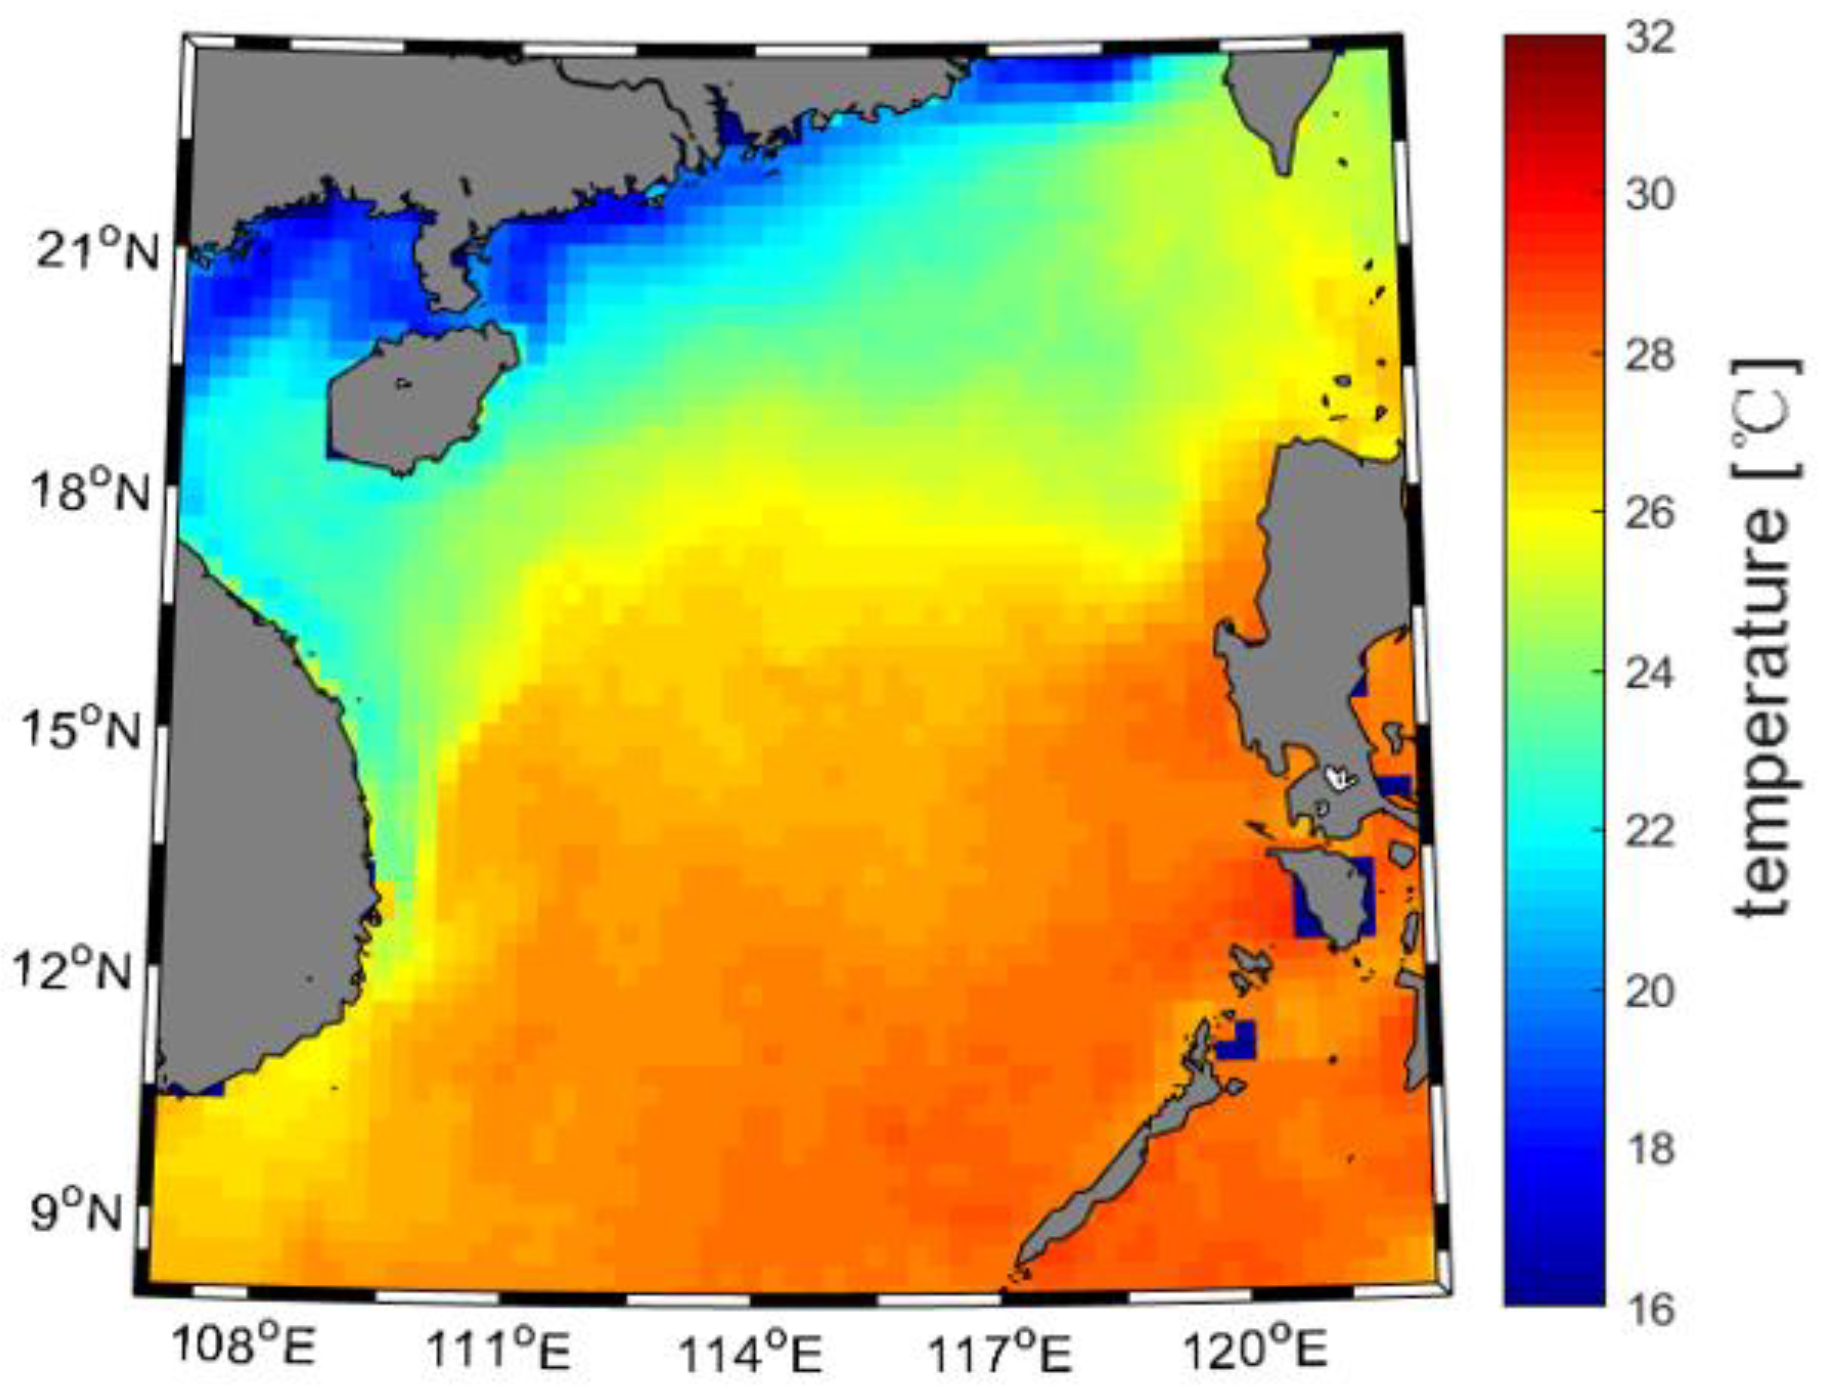
\includegraphics[width=0.9\linewidth]{figures/chapter-1/jmse-11-01030-g001.png}
        \caption{Geospatial data South China sea (Source \cite{jmse11051030})}
        \label{fig:geo-spatial-data-south-china-sea}
    \end{minipage}\hfill
    \begin{minipage}{0.45\textwidth}
        \centering
        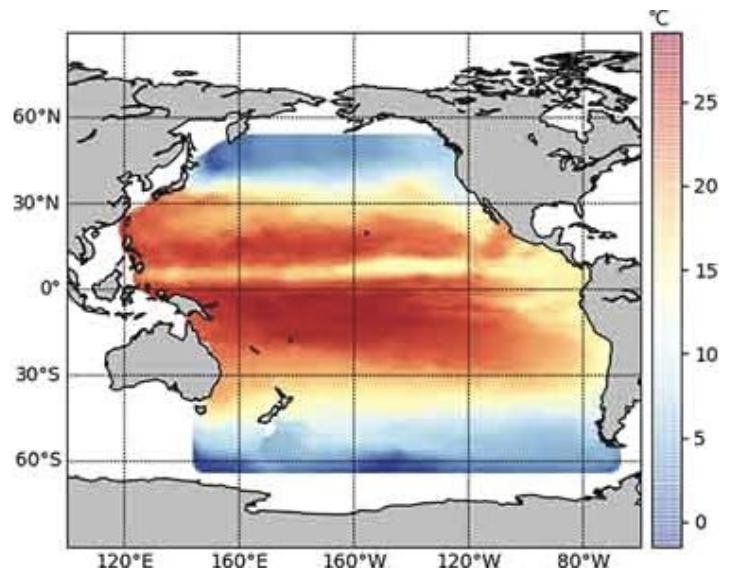
\includegraphics[width=0.9\linewidth]{figures/chapter-1/pacific_ocean.png}
        \caption{Geospatial data Pacific ocean (Source \cite{8913542})}
        \label{fig:geo-spatial-data-pacific-ocean}
    \end{minipage}\hfill
\end{figure}

The above figures shows, that specific areas are considered, South China sea and Pacific Ocean respectively. The data in use is in its premitve form, considering the latitudes and longitudes of these specific regions. While specific regions are considered, there is still a need for a global representation of the data.

When studying the global phenomenon in climate research, it is essential to take into account the actual characteristics of the suface of the planet. To fully understand the problems of the global scale, it is essential to accurately depict the global geospatial data on a model that portrays the true nature of the Earth's surface.

Various methodologies have been employed in the literature to address the problem of global representation, and some use different topological surfaces. One such approach \cite{Weyn_2020} involves the utilization of a cubed sphere, which consists of six faces generated based on the data under consideration.
Within this paper \cite{DBLP:journals/corr/abs-2012-15000}, an architecture named DEEPSPHERE is proposed which is a graph based spherical convolutional neural network.
Even though these deep neural network architectures produce results that are on par with the current state-of-the-art models. These architectures still distort the actual representation of the Earth's surface.
While the issue of accurate representation is still there, these models' heavy usage of GPUs and hardware and longer training time begs the question of finding a simpler model that could represent the global geospatial data and encompass the Earth's surface.

This search of a model which could be used for the representation of the Earth surface motivates us to have a deeper dive in the map projections and their use in the analysis of the geospatial data on the global scale. Map projections are the planar projections of the planet Earth, but these planar projections are generated by complex mathematical calculations. Mainly, map projections are used for the visulization of the geospatial data but their usage for the geospatial data analysis is not conducted thoroughly.


\begin{figure}[h]
    \centering
    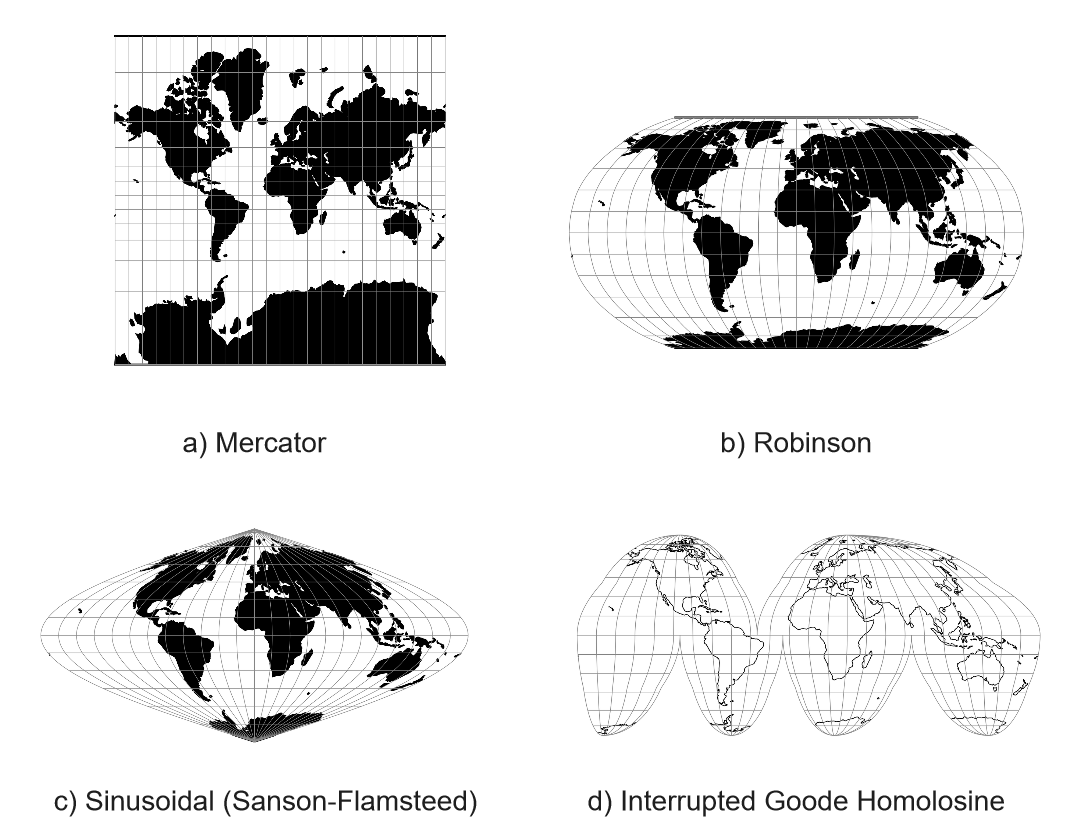
\includegraphics[width=1.0\linewidth]{figures/chapter-1/multi_projections.png}
    \caption{Different map projections (Interal images taken from the source \cite{PROJ_SITE}) }
    \label{fig:multiple-projections}
\end{figure}

The above image show four different projections, but there are numerous map projections, the use of these map projections depend on the problem which is being tackled.

Map projections could be a better candidate for the study of the global geospatial data. The planar nature of the map projections are best suited to be studied by the convolutional neural networks. We can consider a specific map projected geospatial data as a grid, which could be analyzed by the CNNs.
Map projected data could be easily transformed into tensors. This property helps us to use the power of GPUs, making the training process faster. This is the reason convolutional neural networks (CNNs) are considered for the experimentation.

The thesis is of an exploratory nature which studies the effects of the convolution operation on different map projections. It also provides a framework for verifying the effects of the convolution operations on different map projection.
The thesis tries to answer the questions, if map projections are used for the geospatial data analysis, from the selected map projections which of them are a better suited for the task.


\clearpage
\cleardoublepage

\chapter{Geographical Earth Model}

\section{Earth Model}

The shape of the Earth has always intrigued us, leading to the development of various models over the centuries to precisely define its measurements and structure.
The primary motivation behind determining the planet's shape stems from the practical considerations of navigation, where knowledge of true distances and directions is essential.
In modern times, we not only travel from one point to another on the planet but also generate data with precise positions for further analysis of different phenomena.
Mostly, a spherical Earth comes to the mind, which is not the true shape of the Earth as depicted in Figure \ref{fig:earth-image}.

\begin{figure}[h]
    \centering
    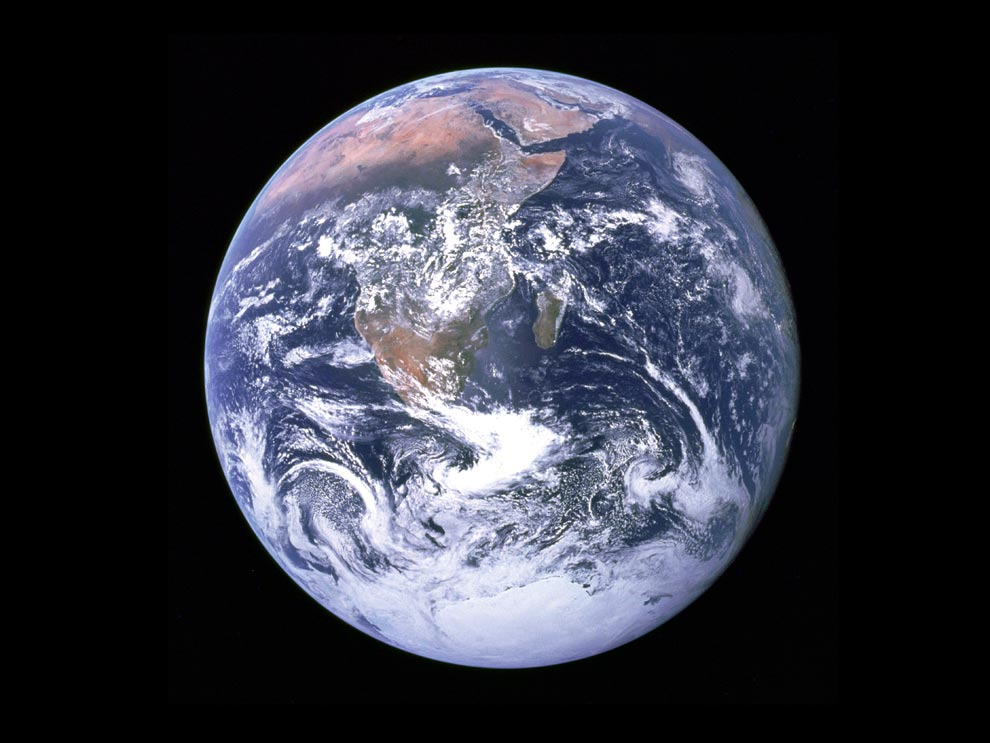
\includegraphics[width=0.5\linewidth]{figures/chapter-2/earth.jpg}
    \caption{The Blue Marble (Source \cite{EARTH_IMAGE}) }
    \label{fig:earth-image}
\end{figure}


To define the shape of any given surface, observations and a mathematical model are employed to establish its dimensions.
This is also true when it comes to defining the figure of the Earth, which exhibits irregularities due to variations on its surface.
Irrespective of our position on the surface of the planet, there are likely to be heights and depressions. When considering only the land mass, we can observe diverse mountain ranges spanning the globe, defined by peaks and valleys.
With all of these irregularities, determining the true shape of the Earth becomes a difficult task.
While we may consider the oceans as a flat surface (acknowledging the presence of uneven shapes at their bottom), the issue of land mass coverage remains.

These questions surrounding the actual shape and dimensions of the Earth fall within the realm of Geodesy, a scientific field concerned with accurately measuring and
determining the Earth's geometry, orientation in space, and gravitational field as defined by National Oceanic and Atmospheric Administration (NOAA) \cite{GEODESY}.
For conducting these measurements, simpler mathematical models are defined by the geodesists which are used to capture the most obvious features of the Earth.

The irregular nature of our planet makes it difficult to define through mathematical models.
Consequently, there is a necessity to investigate a less complex model that portrays the Earth's rugged and uneven surface, which can be characterized by a mathematical model
and simplifies computations.

\section{Geoid Model}
Geoid Model is defined by the average global sea level and is utilized for precise measurements of surface elevations \cite{NOAA_GEOID}.

This model serves as a theoretical representation that aims to address the irregularities found on the actual Earth's surface. To calculate the mean sea level (MSL), we need to average the actual sea levels on the global level.
As the majority of the Earth is covered by oceans, but also features substantial land masses, it is crucial to account for both when conducting these calculations.
This can be achieved by hypothetically filling the land masses with oceanic waters, thereby considering the resulting water surface as the mean sea level on land. Despite the seemingly straightforward nature of constructing the geoid model, researchers are actively gathering data and developing methods to accurately depict this model.

National Aeronautics and Space Administration (NASA)'s GRACE Mission and the European Space Agency (ESA)'s GOCE missions are separately measuring the Earth's gravity field that helps in the calculations for generating the geoid model.
In the field of geodesy this geoid model plays an important role for making calculations and determine positions on the surface of the Earth. Moreover, the study of the geoid
extends beyond geodesy and is also pertinent to climate research \cite{GISGEO_GEOID}.
The geoid model is considered the true representation of the Earth's surface and shape.

\begin{figure}[h]
    \centering
    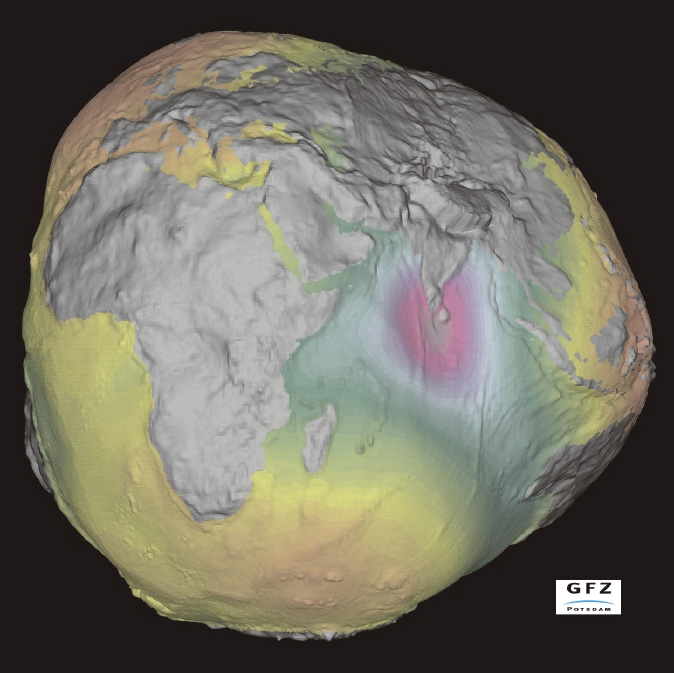
\includegraphics[width=0.7\linewidth]{figures/chapter-2/geoid.jpg}
    \caption{Geoid: The Potsdam Gravity Potato (Source \cite{GEOID_IMAGE}) }
    \label{fig:geoid-image}
\end{figure}

Still the geoid, as depicted in Figure \ref{fig:geoid-image}, is not a smooth surface that makes it impossible for making direct calculations.
Although the irregularities in the Earth's shape have been somewhat mitigated, they still persist to some extent. Thus, the need for a simpler model to accurately
represent the Earth remains for geospatial data analysis.


\section{Spherical Model}

The notion that the Earth possesses a spherical shape was initially posited by the ancient Greeks. Aristotle proposed the idea of a spherical Earth as
mentioned by Johns et. al. in their publication "The Figure of the Earth" in 1959 \cite{Johns1959-og}.

Although, Spherical model of Earth is not a true fact but it provides a framework for gauging dimensions and establishing geographical coordinates.
The spherical model not only simplifies the underlying geoid model as it removes the irregularities of the geoid but also it eased the way to create the coordinate reference
system which depends on latitudes and longitudes.
These latitudes and longitudes are further being utilized in pointing the position of part of the Earth.

\begin{figure}[h]
    \centering
    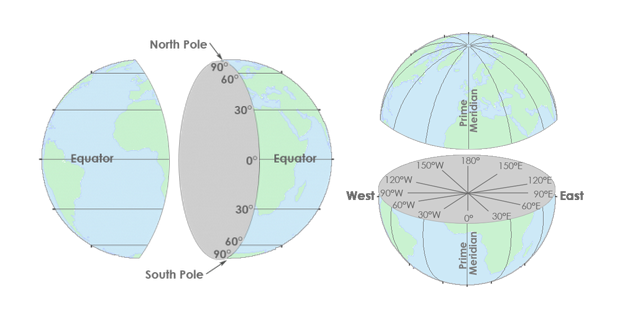
\includegraphics[width=0.7\linewidth]{figures/chapter-2/lat_lon.png}
    \caption{Depiction of Latitudes and Longitudes (Source \cite{GISGEO_LatLon}) }
    \label{fig:shpere-image}
\end{figure}

The latitudes and longitudes are calculated as angles from the equatorial line and the prime meridian respectively. By the advancement of our understanding of the
shape of the earth, we have came to a conclusion that sphere is not the actual representation of the Earth. By studying the gravitational field of the Earth a
correction is needed which bring us to the representation which is now being used for not only making correct positioning of points on Earth,
but this representation is also being used for creating maps.

\section{Ellipsoid Model}

\begin{figure}[h]
    \centering
    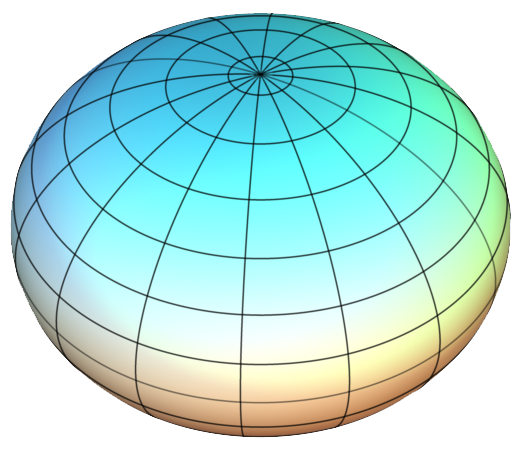
\includegraphics[width=0.4\linewidth]{figures/chapter-2/elipsoid.png}
    \caption{An Ellipsoid (Source \cite{GISGEO_Ellipsoid}) }
    \label{fig:ellipsoid-image}
\end{figure}
After the discovery of the gravitational force, Newton proposed that the Earth is a oblate spheroid or an ellipsoid. This representation of the Earth was confirmed using careful measurements \cite{Osserman2006-ys}. The Earth's ellipsoid depiction serves as a straightforward model that, much like the spherical approximation, streamlines the computations involved in analyzing geospatial data.
This model overcomes the issue of the irregular surface shape of the geoid.

\subsection{Relationship between the ellipsoid and the geoid model}
The geodesists opt for the ellipsoid model over the spherical model when establishing a coordinate reference system because it better represents the Earth's shape.

\begin{figure}[h]
    \centering
    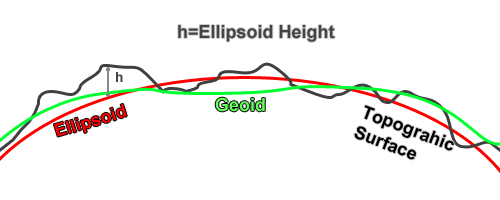
\includegraphics[width=0.6\linewidth]{figures/chapter-2/Ellipsoid-height-relation.png}
    \caption{Relationship between the geoid model and reference ellipsoid(Source \cite{GISGEO_Ellipsoid}) }
    \label{fig:relationship-ellipsoid-geoid-image}
\end{figure}

The generation of coordinate pairs is influenced by the relationship between the ellipsoid and the geoid model. A suitable reference ellipsoid is selected as a close approximation of the underlying geoid model.
When dealing with specific regions different countries use reference ellipsoids which best fit the region of the countries.
World Geodetic System (WGS84) provides a reference ellipsoid which accommodate the whole Earth's geoid \cite{GISGEO_Ellipsoid}. This reference ellipsoid brings the coordinate system (pairs of latitudes and longitudes) which is used for navigation,
reference points on the Earth's surface and geospatial data is mostly collected using the coordinate system which uses the its reference ellipsoid.
GPS global positioning system uses WGS84 as well \cite{GISGEO_WGS84}.

Even though the above models approximate the shape and the dimension of the Earth, we still need the depiction of the Earth which could be used in the analysis of the geospatial
data using convolutional neural networks.


\clearpage
\cleardoublepage

\chapter{Map Projections}
Our search for a simpler model which depicts the Earth's surface which could represent the whole globe has lead us to map projections.
There are numerous map projections, which are being used to represent for different areas of the Earth. An preliminary overview to the map projections is needed and how map projections are generated and how Earth's models eplained in the previous section are related to map projections.

A map projection is a way to represent some part or the whole surface of the Earth on a two dimensional plane, this procedure of mapping the three dimensional surface to a plane is done using mathematical calculations.
Map projections brings us a to represent the whole Earth but each and every map projection is sujected to distortions in shape, area, angles and distance. If one of the map projection try to minimize or mitigate one or two of the distortions, that projection would still be sujected to a distortion.

\section{Generation of Map Projections}
The creation of the map projections require us the usage of \textbf{developable surfaces}. The charateristic which is required for creating the map projections is that they can be mapped onto a two dimensional plane isometrically\cite{Patrikalakis_Maekawa_2010}.
There are three major types of developable surfaces, cylinder, cone, and plane which are used for generating map projections.

The general procedure for generating a map projection is that we first select a geoid model and a reference ellipsoid for approximating the underlying geoid. After the approimation using the geoid then a developable surface is selected from the above mentioned developable surfaces.
Then wrapping the globe with the developable surface gives us the desired map projection.

\begin{figure}[h]
    \centering
    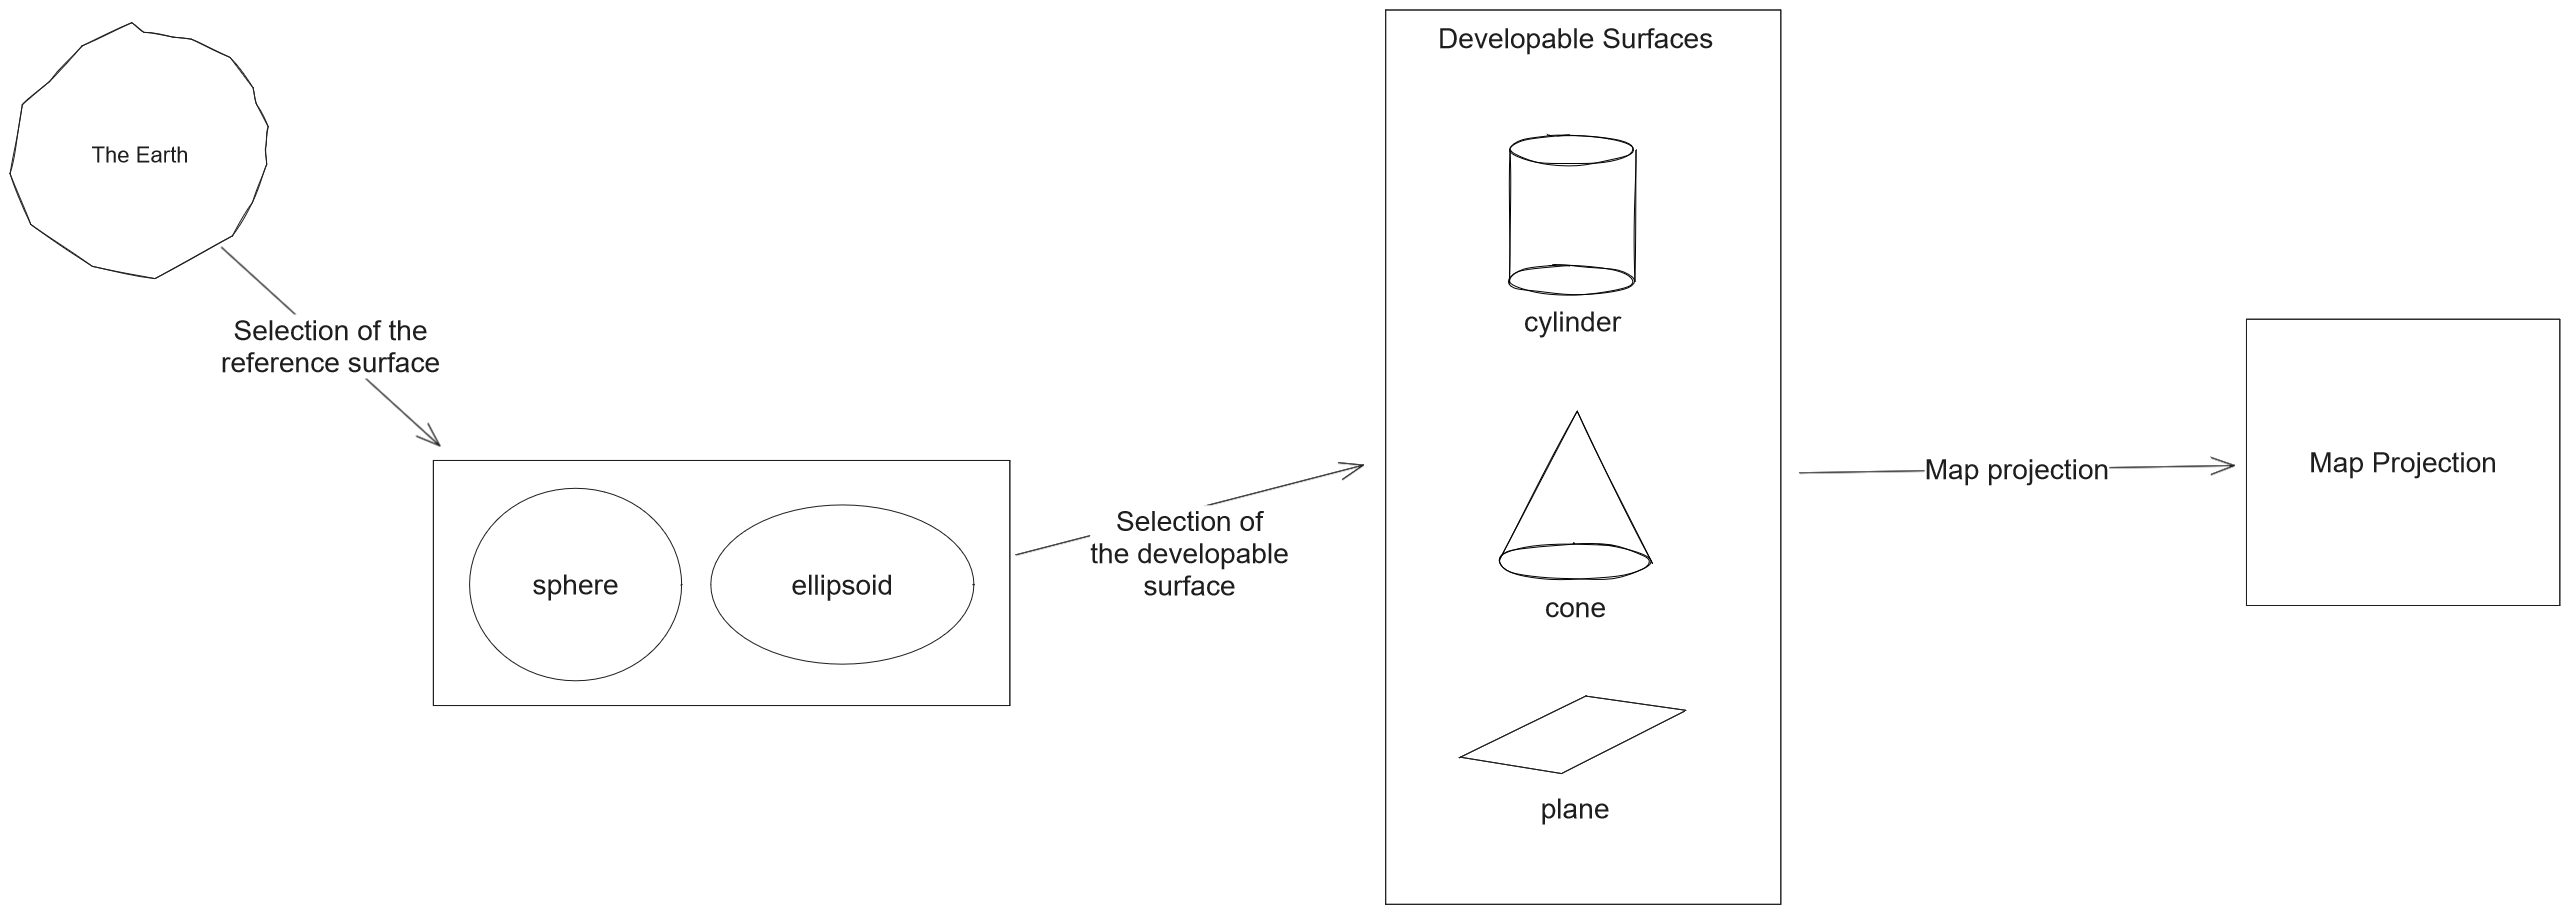
\includegraphics[width=1.0\textwidth]{figures/chapter-3/map_projection_creation.png}
    \caption{Map projection generation flowchart  }
    \label{fig:earth-image}
\end{figure}
\newpage
\section{Types of Map Projections}

The map projections are classified on the bases of the developable surface used for their creation. There are three major types of map projections

\begin{itemize}
    \item Cylindrical Projections
    \item Conic Projections
    \item Azimuthal(Planar) Projections
\end{itemize}

There is another type of projections name \textbf{PseudoCylindrical} projections which are used for the analysis in the experimentation phase.
\subsection{Cylindrical Projections}


\begin{figure}[h]
    \centering
    \includegraphics[width=0.5\textwidth]{figures/chapter-3/merc.png}
    \caption{Mercator Map Projection (Source \cite{PROJ_SITE})}
    \label{fig:mercator-image}
\end{figure}

Cylindrical map projections are generated when the Earth is enveloped by a cylinder, same as we place the globe at the center. All of the longitudnal lines will be projected on the cylinder as perpendicular lines to the equator and the latittudnal lines  will be parallel to the equator. If we cut the cylinder at any of the longitude we have a cylindrical projection \cite{Snyder1982}.

In the image above Mercator projection is shown, which has conformal property (preserves the shape and the angles), but the size of the land mass is distorted at the polar regions \cite{GISGEO_Cylinder}. Where Greenland is bigger than African continent, in reality that is not true.

\newpage
\subsection{Pseudocylindrical Projections}

\begin{figure}[h]
    \centering
    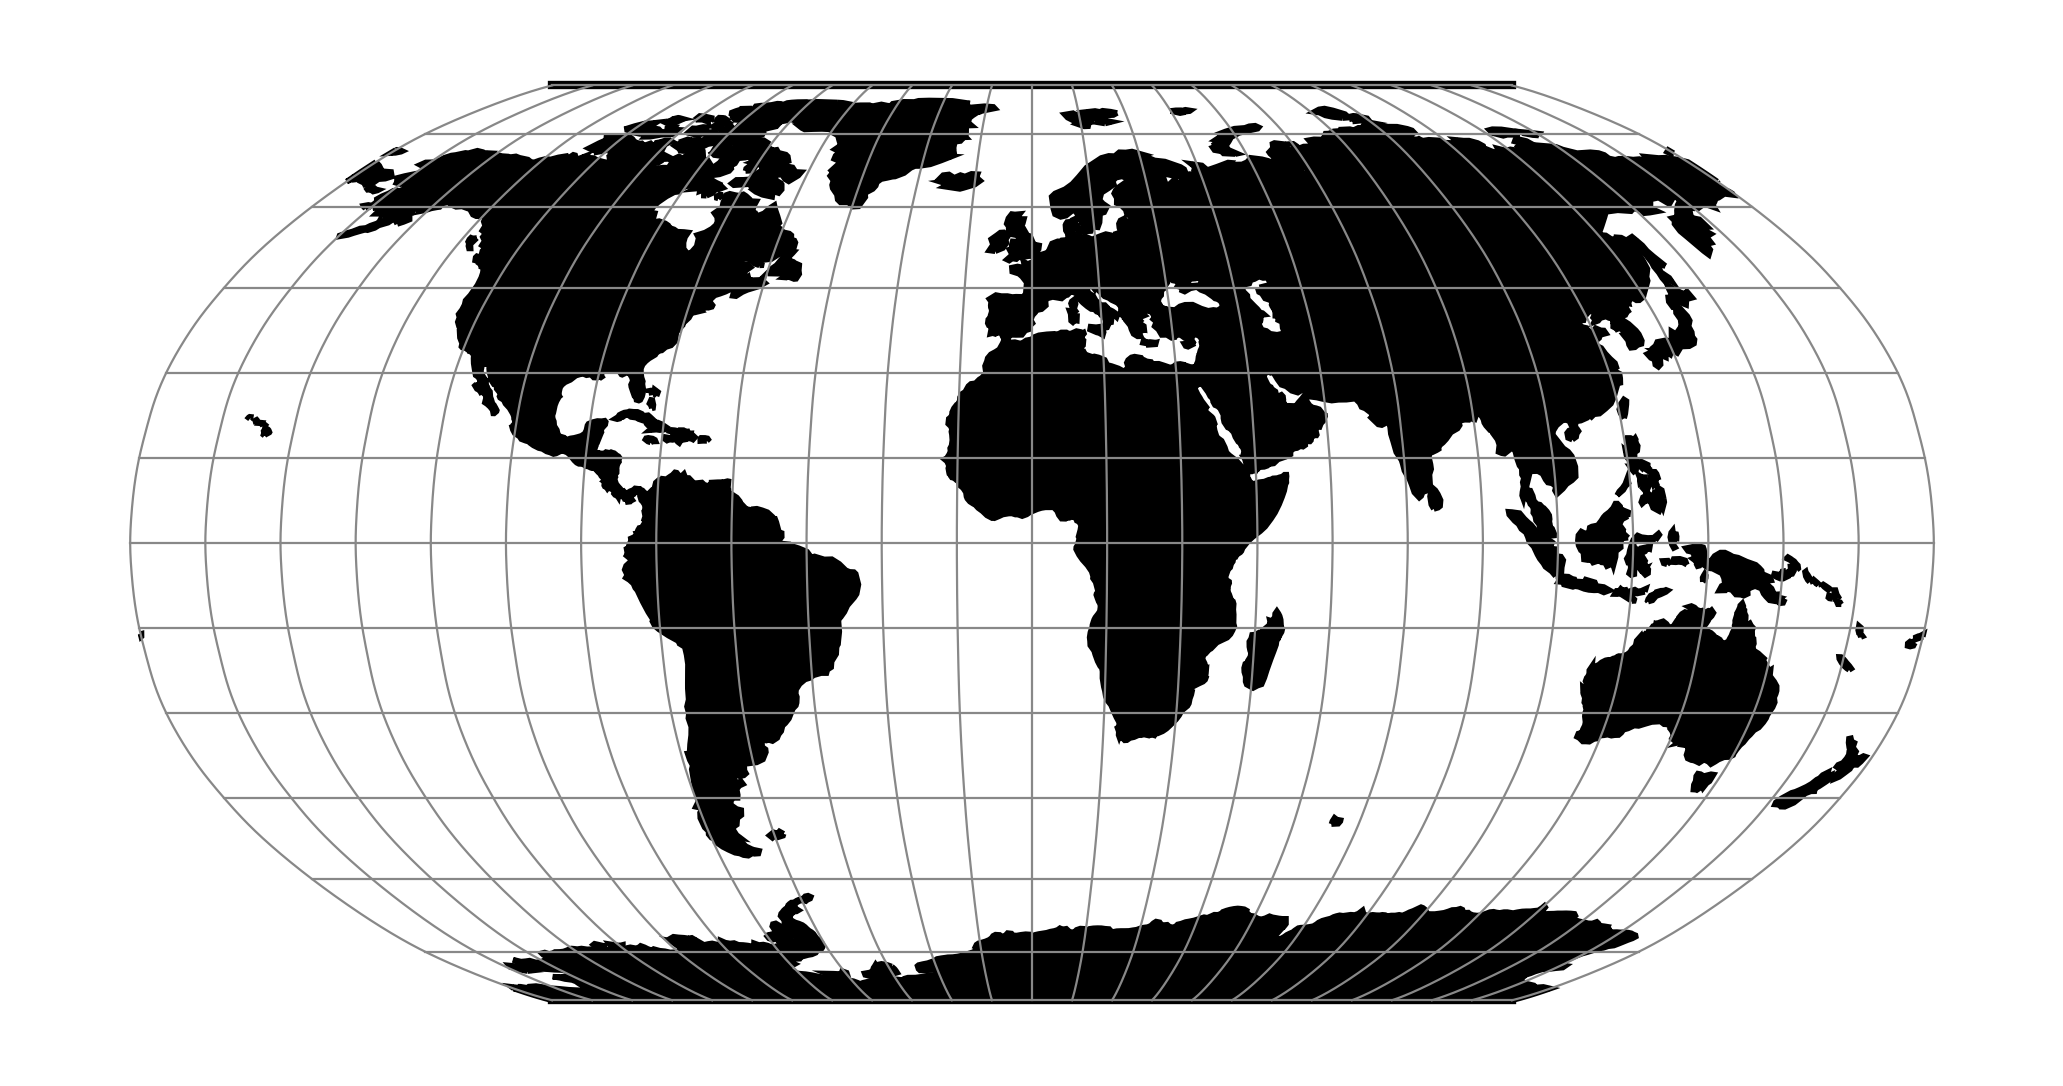
\includegraphics[width=0.5\textwidth]{figures/chapter-1/robinson.png}
    \caption{Robinson Map Projection (Source \cite{PROJ_SITE})}
    \label{fig:robinson-image}
\end{figure}


These projections are generated using the same method as cylindrical projections are created but the longitudnal lines are curved other than the prime merdian but the latitudnal lines are parallel to the equator \cite{GISGEO_Cylinder}.
The above image shown is the robinson projection which is a pseudocylindrical projection.

\subsection{Conic Projections}

\begin{figure}[h]
    \centering
    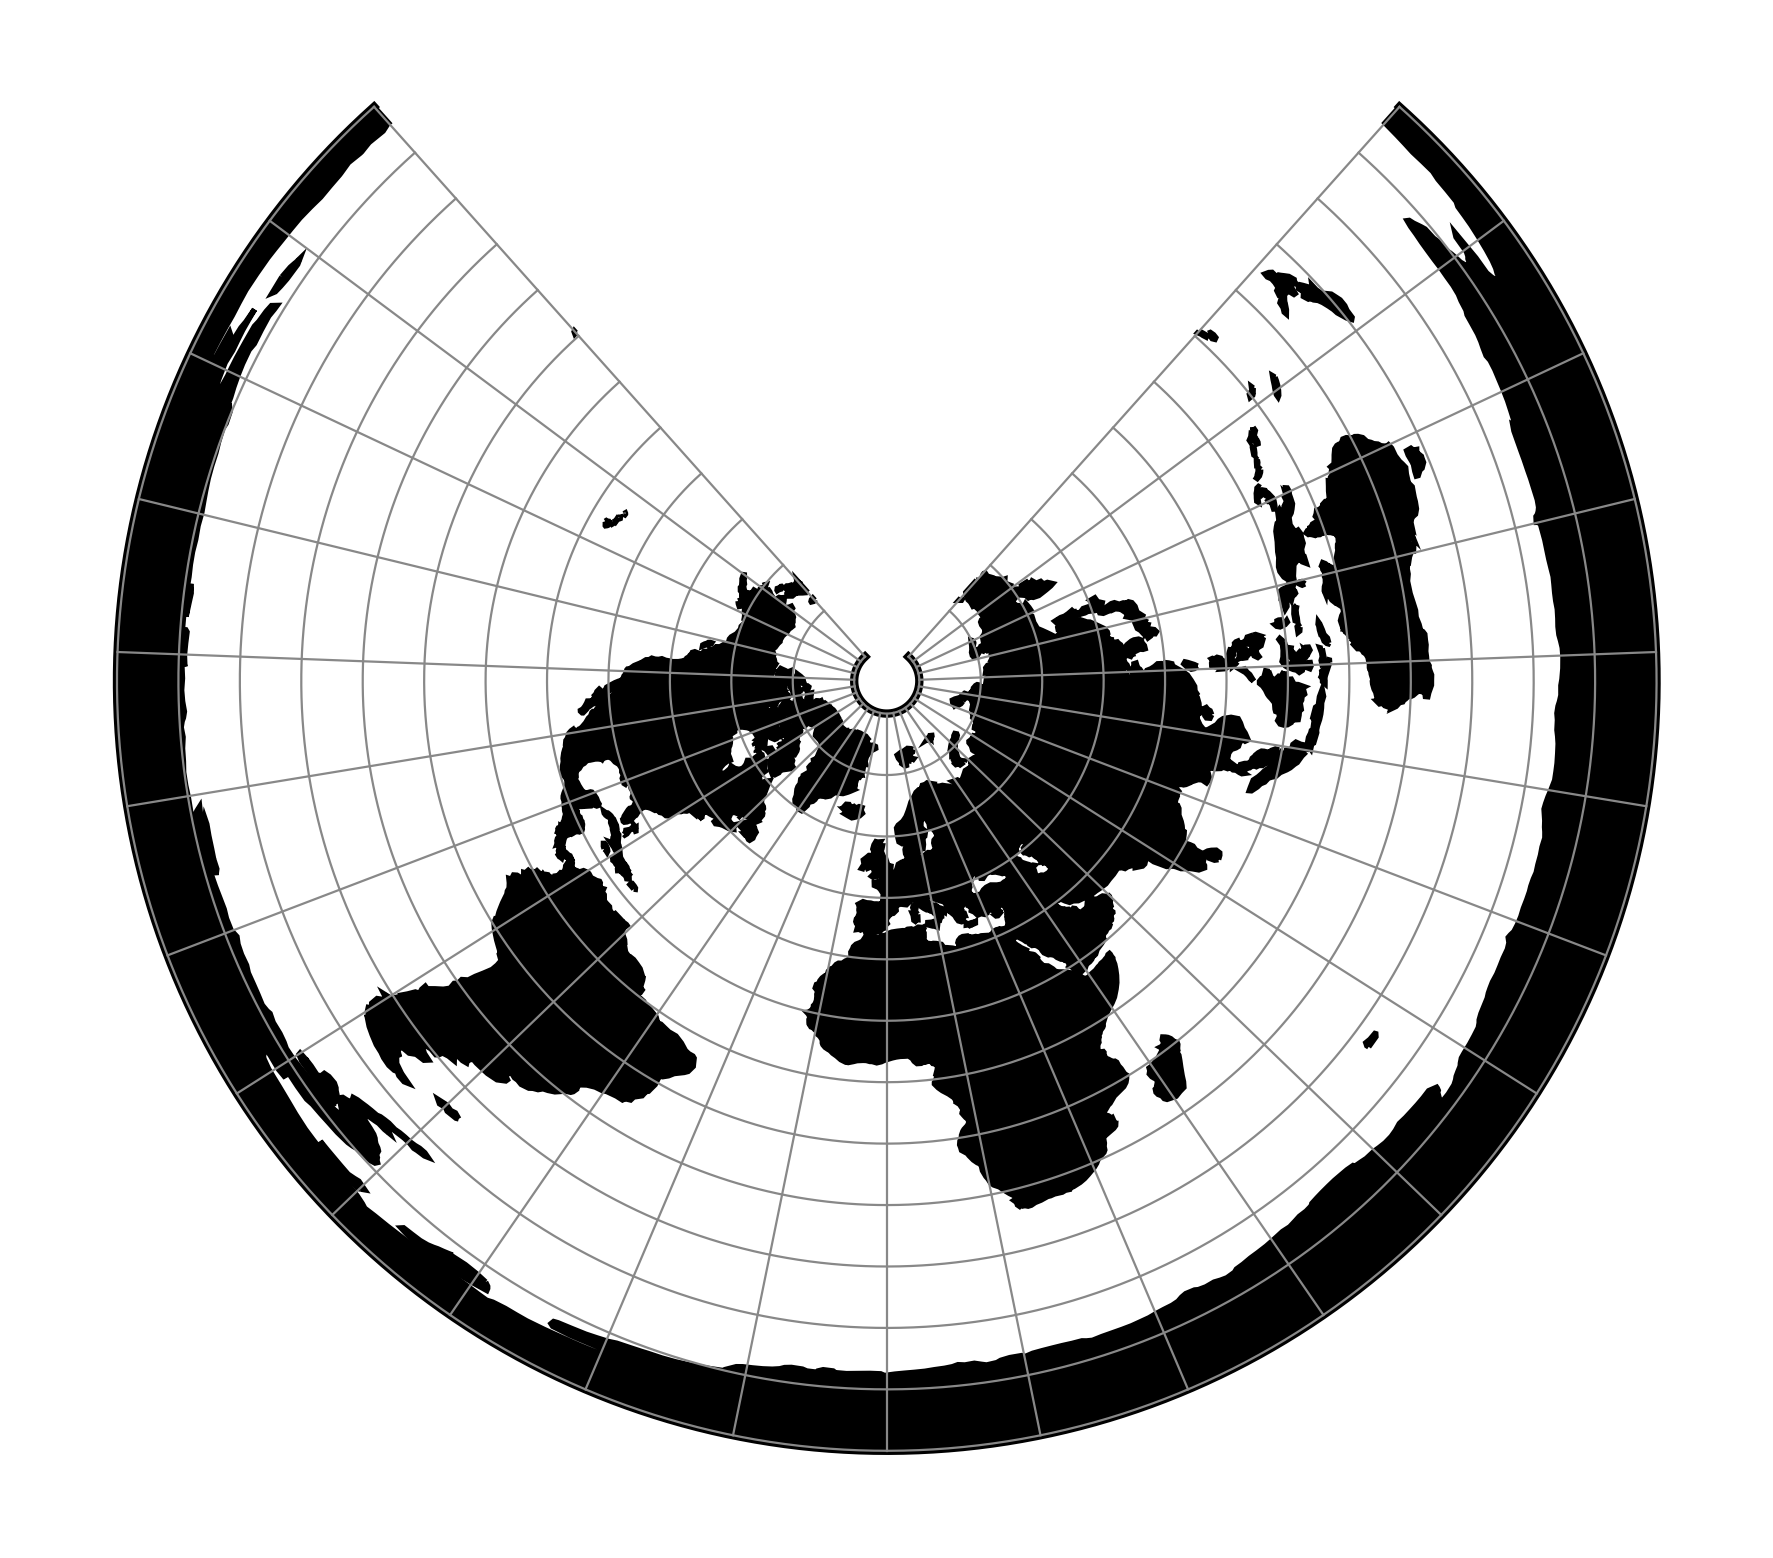
\includegraphics[width=0.5\textwidth]{figures/chapter-3/vitk1.png}
    \caption{Vitkovsky I Map Projection (Source \cite{PROJ_SITE})}
    \label{fig:vitkovsky-image}
\end{figure}
Conic projections are formed by situating a cone atop the Earth's pole and completely enveloping the Earth within the cone. Consequently, the longitudnal lines remain linear, while the latitudnal lines become arcs that revolve around the apex of the cone. Upon severing the cone along any given longitudnal line, a conic projection is thereby produced \cite{Snyder1982}.

\newpage
\subsection{Planar Projections}

\begin{figure}[h]
    \centering
    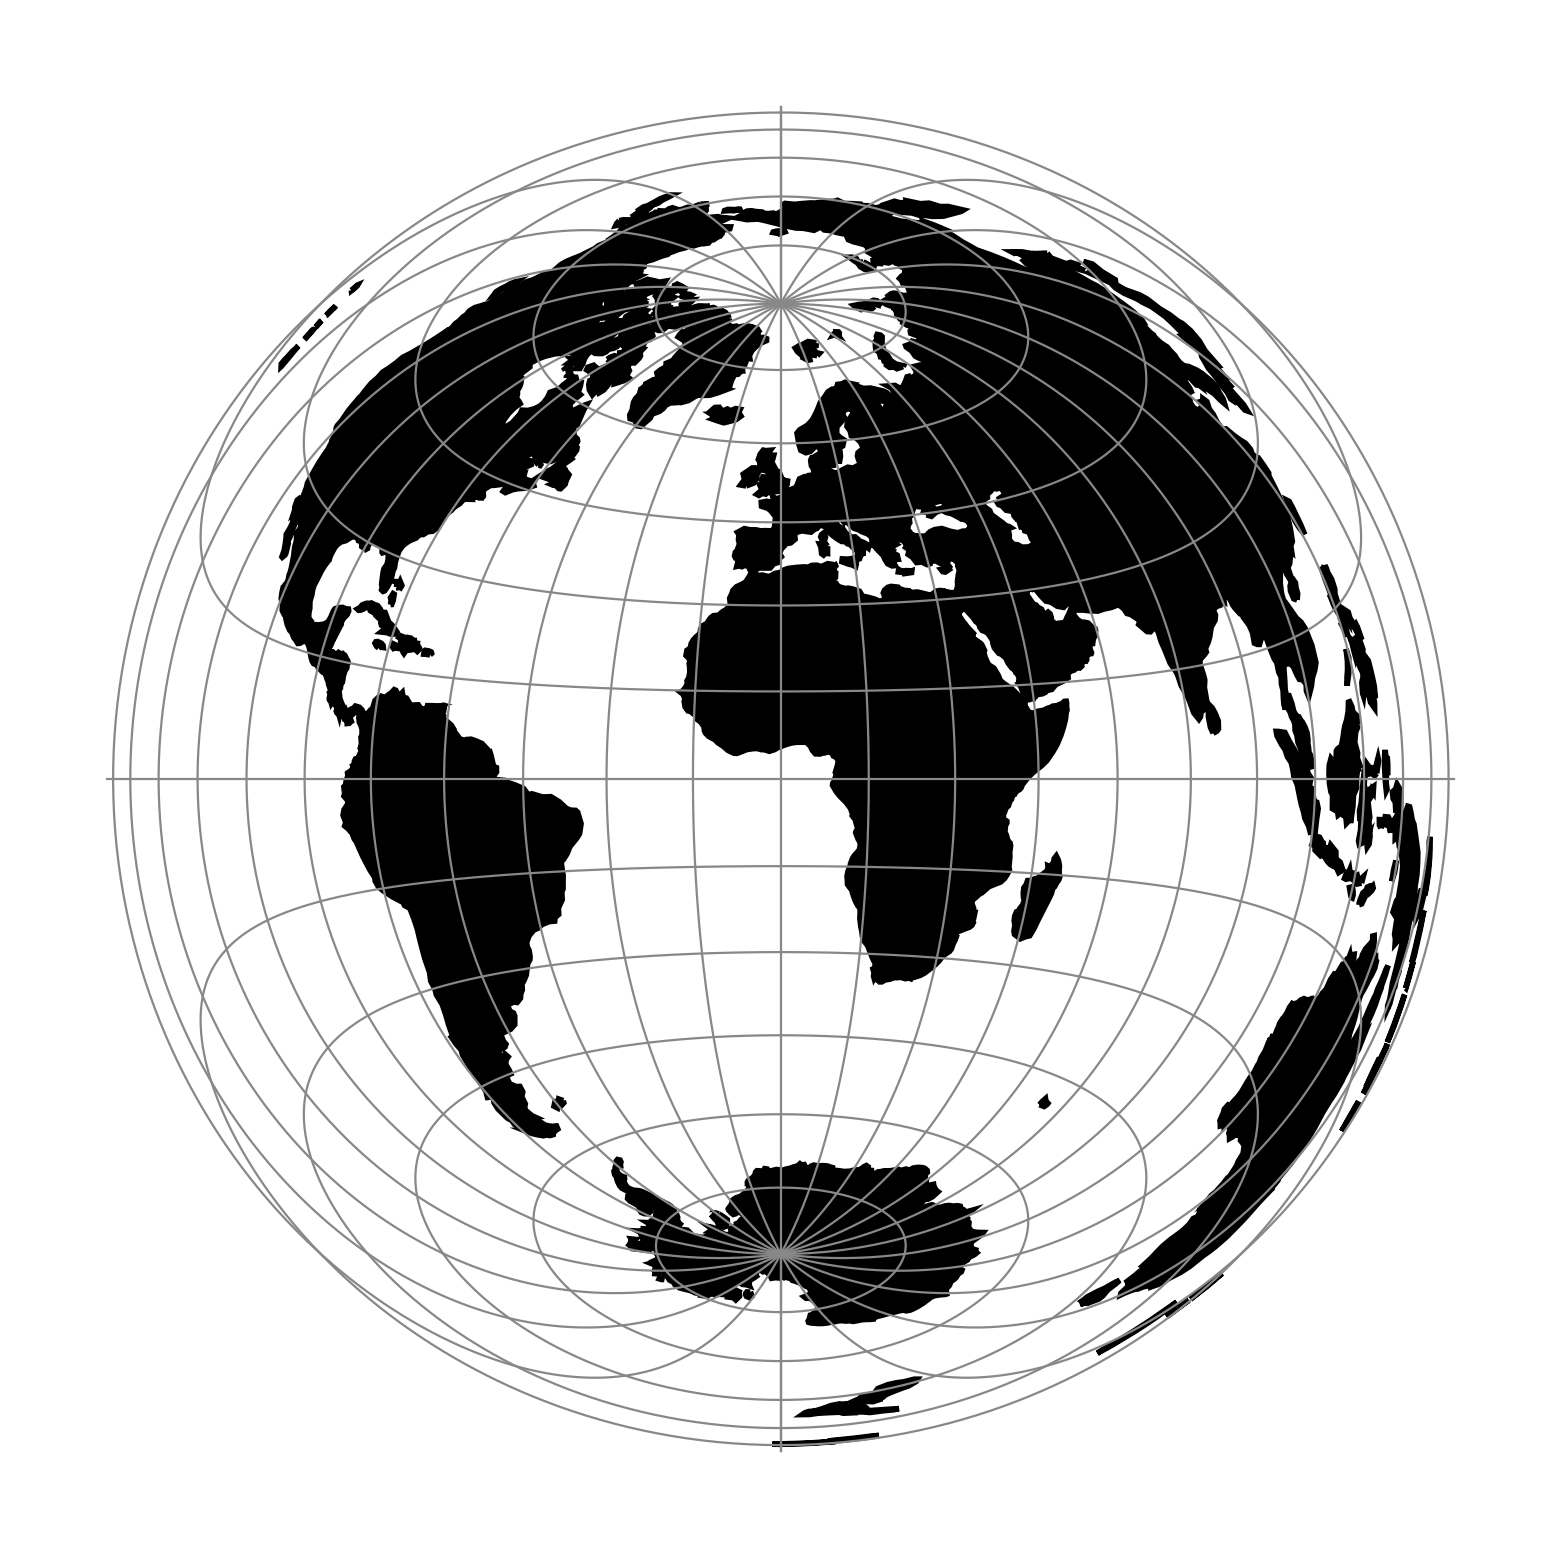
\includegraphics[width=0.5\textwidth]{figures/chapter-3/laea.png}
    \caption{Lambert Azimuthal Equal Area Map Projection (Source \cite{PROJ_SITE})}
    \label{fig:vitkovsky-image}
\end{figure}

planar projections are formed when the plane is positioned at one of the Earth's poles and is tangent to the sphere. Consequently, the projection of the sphere becomes azimuthal. In this scenario, the longitudinal lines will appear as straight lines originating from the point of tangency \cite{Snyder1982}.


\section{Map Projections and Distortions}
\begin{figure}[h]
    \centering
    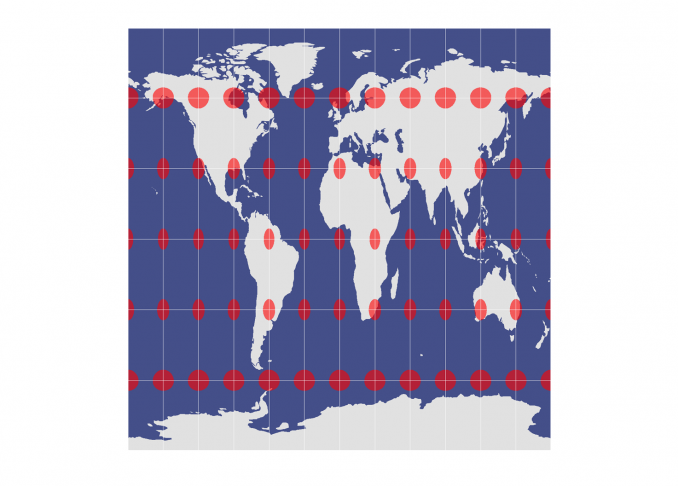
\includegraphics[width=0.5\textwidth]{figures/chapter-3/Tissot-Equidistant-Cylindrical-1-678x486.png}
    \caption{Tissot's Indicatrix on Equidistant Cylindrical Projection (Source \cite{GISGEO_Tissot})}
    \label{fig:tissot-image}
\end{figure}
Whenever a three dimensional geometric shape is projected to a two dimentional geometric shape, there will be distortions. same is the case with the map proections which are projection of our three dimensional Earth to two dimensional plane.
The distortions in map projections can be categorized into four types:
\begin{itemize}
    \item Area distortion
    \item Direction distortion
    \item Shape distortion
    \item Distance distortion
\end{itemize}

To gain a better understanding of these distortions, Tissot's indicatrix can be utilized, it visually demonstrates the distortions by depicting ellipses, known as indicatrices, which change their shape to represent the distortions \cite{Snyder1982}.
\begin{itemize}
    \item The preservation of local angles and shapes is ensured through the utilization of conformal map projections \cite{GISGEO_Tissot}.
    \item The preservation of the relative size of areas is achieved through the utilization of Equal Area Projections \cite{GISGEO_Tissot}.
    \item The distance on certain set of lines is preserved by Equidistant Projections \cite{GISGEO_Tissot}.
\end{itemize}
Figure ~\ref{fig:tissot-image} shows the tissot's indicatrix on the Equidistant Cylindrical projection which tries to preserve distances along the equator and the longitudnal lines only \cite{GISGEO_Tissot}.

\clearpage
\cleardoublepage

\chapter{Related Work}
\label{chap:related_work}
As we traverse the intricate terrain of geospatial data analysis in the realm of global Earth system models,
it becomes of utmost importance to have a comprehensive grasp of the existing methodologies and advancements.
This chapter starts on an extremely thorough investigation of the seminal works and groundbreaking research that
have laid the foundation for the utilization of Convolutional Neural Networks (CNNs) in geospatial analysis.
It delves deeply into the evolution of convolutional architectures, highlighting their application in various scientific
fields beyond conventional image processing, encompassing their transformative potential in climatology, oceanography, and meteorology.
By thoroughly analyzing both Euclidean and non-Euclidean convolutional operations, this discussion aspires to offer a contextual framework
for the current research within the broader domain of deep learning investigation, highlighting the importance of adapting and optimizing CNNs
to effectively exploit the complex, multidimensional nature of geospatial data.
@TODO: review [usman]
\section{Convolutions On Euclidean Space}
\subsection{Convolutional Neural Networks (CNN)}
With the advent of deep learning models, convolutional neural networks were developed primarily for solving the vision related tasks. These architectures are now being embraced across various scientific disciplines for the purpose of data analysis, owing to their utilization of convolutions.
In case of the climate data studies where the observations obtained are subjected to spatial mapping via latitudes and longitudes, forming a grid like structure which could be analyzed by the Convolutional neural networks.
Computer vision pertains to the examination of images, which are mostly multi-channel grids. In the case of RBG images, an image could be described as three grids stacked together, each grid containing information about a specific color (Red, Blue, Green) for a pixel. Similarly, geospatial data which is relevant under the same latitudes and longitudes mapping could be stacked together for the analysis harnessing the Convolutional Neural Networks (CNN).

Below are the main advatages of using convolutional neural networks:
\begin{itemize}
    \item \textbf{Learnable Kernels}\\
          Convolutional neural networks possess the inherent capability to process \textbf{grid-format} data using 2D convolutions, as presented in \cite{LeChun_5}, where they were used for the MNIST dataset\cite{deng2012mnist} for the hand written digit classification.
          The convolution layer of the network is facilitated by \textbf{learnable kernels}. The learning of the kernels happens due to back propagation as in the gradient base-learning.
          These kernels traverse the image, capturing distinctive features within the gridded data and generating feature maps for subsequent layers in the network to further extract relevant features.

\end{itemize}
\begin{itemize}
    \item \textbf{Preserves Spatial Context }\\
          A drawback of fully connected architectures is their complete disregard for the input's topology. The presentation order of input variables can be arbitrary without affecting the training outcome. Images possess a strong \textbf{local structure}, where spatially adjacent variables or pixels exhibit high \textbf{correlation}. These local correlations contribute to the well-known benefits of extracting and combining local features prior to recognizing spatial objects, such as edges or corners. Convolutional Networks enforce the extraction of local features
          by confining the receptive fields of hidden units to be local \cite{LeChun_5}.
\end{itemize}

\begin{itemize}
    \item \textbf{Shift Invariance}\\
          In the convolutional networks, the property of shift invariance is achieved through the weight configurations being replicated across space\cite{LeChun_5}.

\end{itemize}
\begin{itemize}
    \item \textbf{Tolerance of Transformation }\\
          Convolutional layers possess a core characteristic where the output of the feature map will undergo a shift of the same magnitude as the input image, but remain unaltered in all other aspects. This particular attribute forms the foundation for the resilience exhibited by convolutional networks against shifts and distortions encountered in the input data\cite{LeChun_5}.
          The precise location of a detected feature diminishes in significance once it has been identified. The only relevant aspect is its approximate position in relation to other features \cite{LeChun_5}.
\end{itemize}


\begin{figure}[h]
    \centering
    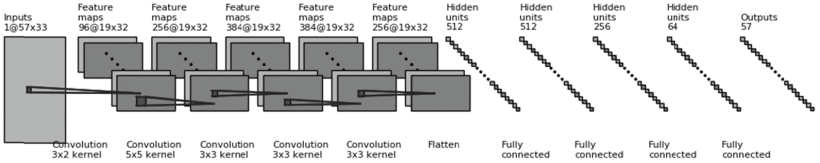
\includegraphics[width=1.0\linewidth]{figures/chapter-4/han3-2955957-large.png}
    \caption{Architecture for estimating subsurface temperatures in Pacific Ocean (Source \cite{8913542}) }
    \label{fig:architecture-pacific-ocean}
\end{figure}

Due to the above mentioned properties, convolutional neural networks are used for the geospatial data as the Figure ~\ref{fig:architecture-pacific-ocean} shows an architecture which is used for predicting the subsurface temperature.
This model is using the grid-format data for capturing the advanced features through the high dimensional data \cite{8913542}. The usage of the convolutional neural networks is also to reduce the time of feature engineering \cite{8913542}.


\subsection{Convolutional Block Attention Module (CBAM)}
Even though the convolutional neural networks perform well in capturing the features in the planar data (grid) but this comes with a cost of creating deeper architectures as VGG16\cite{simonyan2015deep} with more than hundred million trainable parameters, VGG16 was utilized for image recognition task \cite{simonyan2015deep}.

There has been attraction to attention mechanism, which tries to focus on the features extracted by the convolutions which have more data activity.
Since convolution operations combine cross-channel and spatial information to extract informative features, The method proposed \cite{woo2018cbam} focuses on enhancing meaningful features along these two principal dimensions: channel and spatial axes \cite{woo2018cbam}.
The utilization of the attention was separated into two parts first the learning of the channel attention and after that learning the spatial attention \cite{woo2018cbam}. This removes the unwanted clutter and focuses on only the relevant features \cite{woo2018cbam}.

\begin{figure}[h]
    \centering
    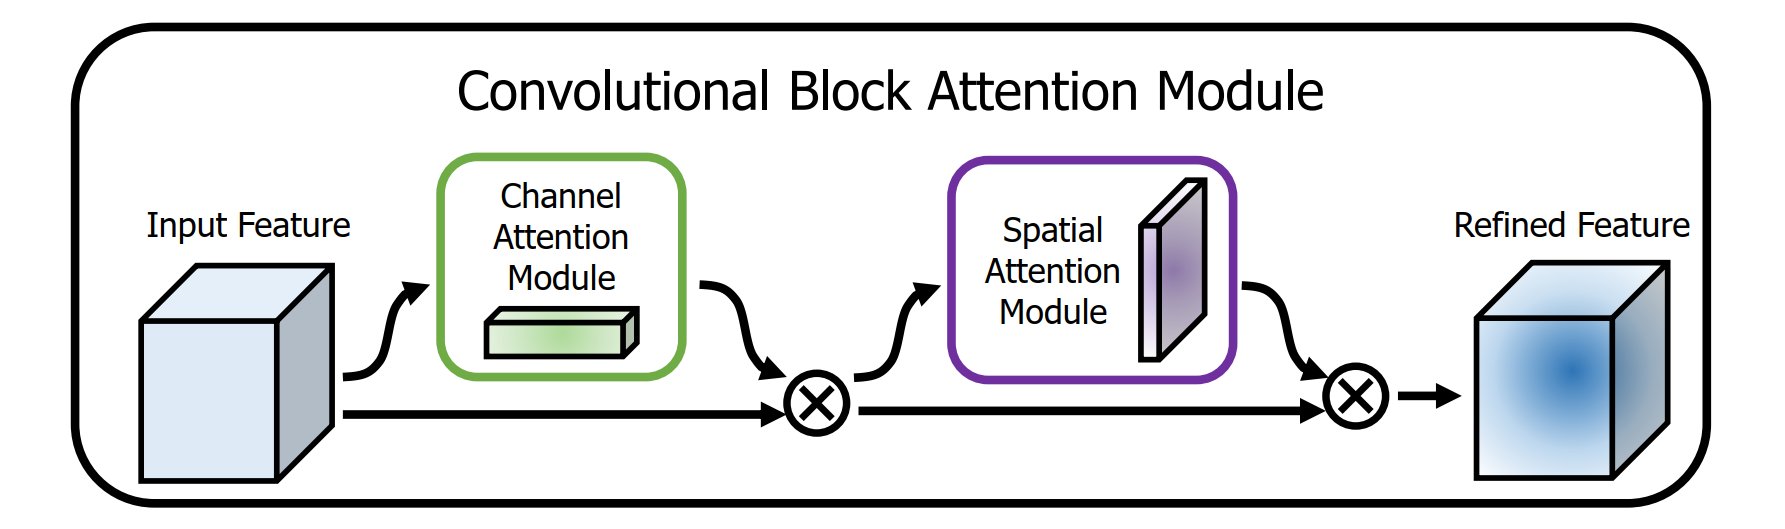
\includegraphics[width=1.0\linewidth]{figures/chapter-4/CBAM.png}
    \caption{Convolutional Block Attention Module (CBAM) (Source \cite{woo2018cbam}) }
    \label{fig:cbam-image}
\end{figure}

Figure ~\ref{fig:cbam-image} depicts the two types of attention modules which applied in a sequential manner for boosting the performance of the network\cite{woo2018cbam}.

In the context of analyzing geospatial data, the utilization of CBAM has proven to enhance performance \cite{mao2023reconstructing}.
The CBAM module utilization is also happening for nowcasting the precipitation \cite{trebing2021smaatunet}. Both \cite{mao2023reconstructing} \cite{trebing2021smaatunet} are being used on the smaller regions of the globe.

\subsection{U-Net}

U-Net architecture was first used in the segmentation task for the medical images. The name of the architecture is because of its shape. This deep neural network architecture incorporates both the encode and the decoder parts in the same architecture. As mentioned the usage of the proposed architecture was to give each pixel of the image a class.


\begin{figure}[h]
    \centering
    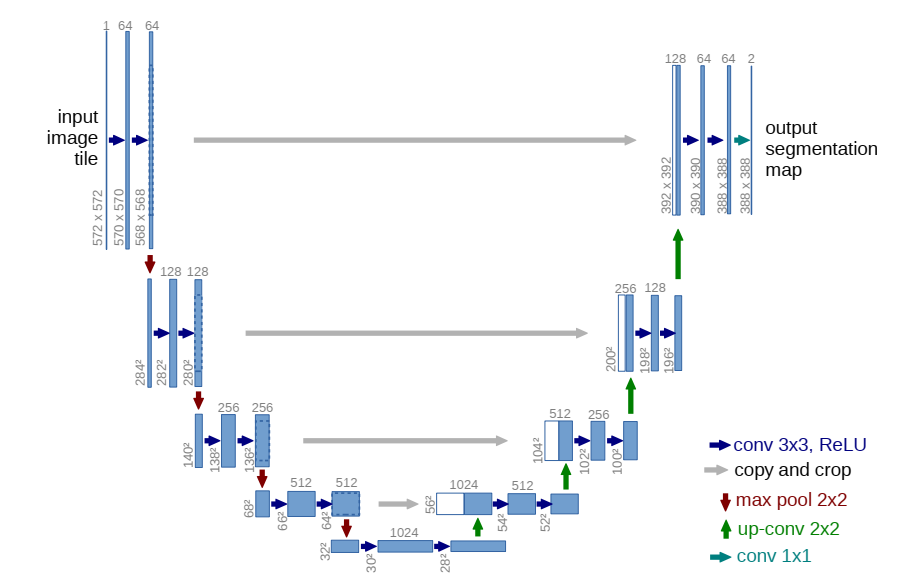
\includegraphics[width=1.0\linewidth]{figures/chapter-4/unet.png}
    \caption{Original U-Net proposed for the segmentation of the medical images (Source \cite{ronneberger2015unet}) }
    \label{fig:unet}
\end{figure}

As seen in figure ~\ref{fig:unet}, the major feature of the architecture is that the left hand side is the contraction part and the right hand side in the expansion \cite{ronneberger2015unet}. Each of the contraction and the expansion block of the network is utilizing double convolutional layers \cite{ronneberger2015unet}.
In order to achieve localization, the upsampled output is combined with high resolution features obtained from the contracting path. Subsequently, a convolution layer is employed to acquire the ability to construct a more accurate output, utilizing the information provided \cite{ronneberger2015unet}.

For the geospatial analysis, rather than giving each pixel a class actual values are generated for the data under consideration \cite{trebing2021smaatunet}. A combination of U-Net and ConvLSTM are used, the U-Net is used to predict the heatwave intensity under the observed area of South China sea \cite{rs15164068}.

\section{Convolutions on Non-Euclidean Space}
The convolutional neural networks were initially designed for the capturing patterns in the Euclidean 2D space, for images which are in the format of a grid. The data is represented in equirectangular grids, which aligns with the nature of the image data.
Currently, various scientific fields are encountering problems related to accurately representing their data. In the past, data in these fields was primarily analyzed by projecting it onto a Euclidean plane before conducting further analysis.
With the advent of Geometric machine learning, new techniques are being developed to study data on non-euclidean spaces. This approach brings the data closer to its actual representation.
Thus it provides the mechanism to perform convolutional operation on the non-euclidean spaces and manifolds

\subsection{Spherical CNN}

In a planar image, the arrangement of patterns can be altered through movement, whereas in the case of patterns on the sphere, their movement is characterized by a three-dimensional rotation rather than a translation \cite{cohen2018spherical}.
The substitution of the definition of cross-correlation or convolution necessitates the substitution of filter translations by rotations \cite{cohen2018spherical}.

The set of movements on the sphere could be described in a three-dimensional space, known as 3D rotations and they can be described as a manifold SO(3) \cite{cohen2018spherical}. When spherical correlation or convolution is performed, the resulting feature map are to be regarded as a signal on SO(3) rather than a signal on the sphere, $S^2$ \cite{cohen2018spherical}.
The efficient implementation of the $S^2$ and SO(3) correlation can be achieved through the utilization of generalized FFT algorithms \cite{cohen2018spherical}.

The feature maps in the spherical convolution are generated at a rotation $R \in SO(3)$ by the inner product of a filter and a feature map using the rotation $R$ \cite{cohen2018spherical}.
For computing the spherical convolutions data and the filters are considered as continuous functions $f: S^2 \rightarrow  \mathbb{R}^K $, K is the number of channels\cite{cohen2018spherical}.
Spherical CNNs provide the rotational equivariance.

The calculation of the spherical convolution can be carried out in the harmonic space by executing matrix multiplications involving the harmonic coefficients of the spherical signal and the filter. This approach is particularly advantageous due to the familiarity of deep learning practitioners with utilizing GPUs to efficiently perform matrix multiplications \cite{towardsdatascienceGeometricDeep}.

\begin{itemize}
    \item \textbf{Parameterized Differential Operators }\\
          This technique performs effective convolutions on the manifolds which are approximated by the underlying meshes.In order to achieve these convolutions, the convolutional kernels that can be learned are reparameterized into a linear combination of differential operators. In this technique the differential operators of different order take place of the cross correlation linear operators to find local features \cite{jiang2019spherical}. This approach is could also be used for modeling the climate data.
          For the experimentation, U-Net based architecture is deployed.

\end{itemize}


\subsection{Spherical U-Net}
This architecture comes from the medical field, where the model is designed for studying the brain as sphere. While the spherical CNN \cite{cohen2018spherical} considers the data as continuous functions, this approach depends on the discretization of the sphere using the icosahedron structure and generating the uniform sphere by hierarchically adding new vertices \cite{zhao2019spherical}.
In \cite{zhao2019spherical}, \textbf{Direct Neighbor (DiNe)} filters and convolutions are proposed which use the consistent neighborhood orders on the spherical space\cite{zhao2019spherical}. Such an approach could be used for the geo science related machine learning tasks. The issue for such tasks would be the discretization of the geo-spatial data on the sphere.


\begin{figure}[h]
    \centering
    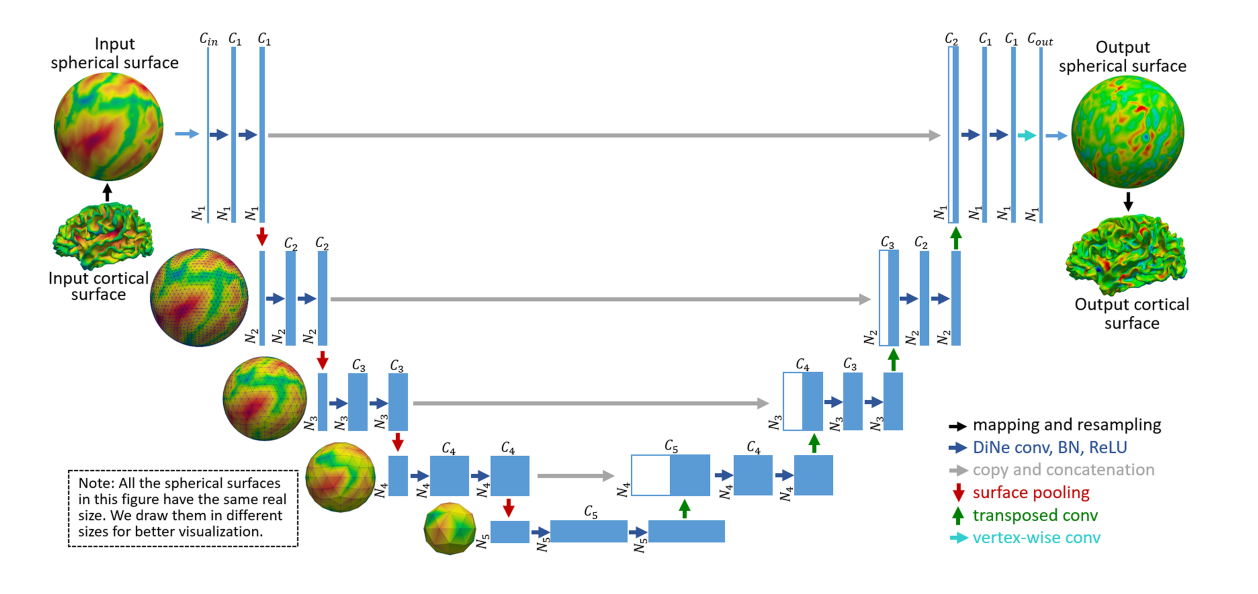
\includegraphics[width=1.0\linewidth]{figures/chapter-4/spherical_unet.png}
    \caption{Spherical U-Net for the brain cortical surface (Source \cite{zhao2019spherical}) }
    \label{fig:spherical-unet}
\end{figure}

\section{Sphere2Vec}
This is an encoder model which is trying to mitigate the distortion of distance that arises from the map projections. This method can encode spherical coordinates by abstaining from the distortions of the map projections and spherical to Euclidean distance approimation errors \cite{mai2023sphere2vec}. 2D Discrete Fourier Transform basis are used in the technique of multi-scale encoding to measure the accurate distances on the sphere \cite{mai2023sphere2vec}. While \cite{mai2023sphere2vec} also argues about the incapability of 2D and NeRF-style 3D location encoders to correctly find spherical distances.

\clearpage
\cleardoublepage

\chapter{Datasets}
\label{chap:dataset}

The data used for experimentation is taken from \cite{willi_rath_2023_7779883} which contains different climate features. The data is generated by the simulations, these simulations are provided by the robust climate Earth models \cite{willi_rath_2023_7779883}.

The dataset provides multiple features which are listed below:
\begin{itemize}
    \item sea surface temperature
    \item surface air temperature
    \item sea level pressure
    \item sea surface salinity
    \item geopotential height (500mb)
    \item precipitation
\end{itemize}

The features that we considered for the experimentation were the geopotential height and precipitation.
Both of the datasets are timeseries data, where measurement for each feature is done by month for a 1000 year. Each of the datasets are explaind in detail for the better understanding of the dataset.
\newpage
\subsection{Geopotential Height Dataset}
It consists of 12000 geo referenced data points, where each geo referenced data point is a grid of (96x192) containing geopotential height value specific to a pair latitude and longitude.
Each geo referenced data point does also contains a time value associated with it as well.

96  is the total number of latitude values and  192 is the total number of longitude values, against which feature data is generated. The total number of geopotential height measurements for each month is 18816.

\begin{figure}[h]
    \centering
    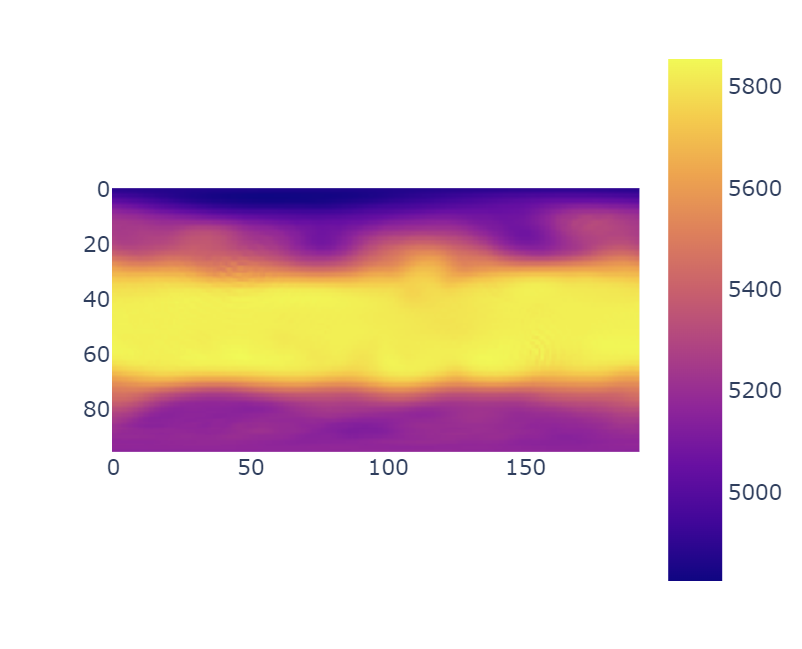
\includegraphics[width=0.6\linewidth]{figures/chapter-5/data_original.png}
    \caption{Original geopotential height 96x192 grid }
    \label{fig:org_geopoth}
\end{figure}

\subsection{Precipitation Dataset}

@TODO: add Precipitation dataset [usman]


\clearpage
\cleardoublepage

\chapter{Geo Spatial Data Pre-processing Pipeline}
\label{chap:preprocess}
\begin{figure}[h]
    \centering
    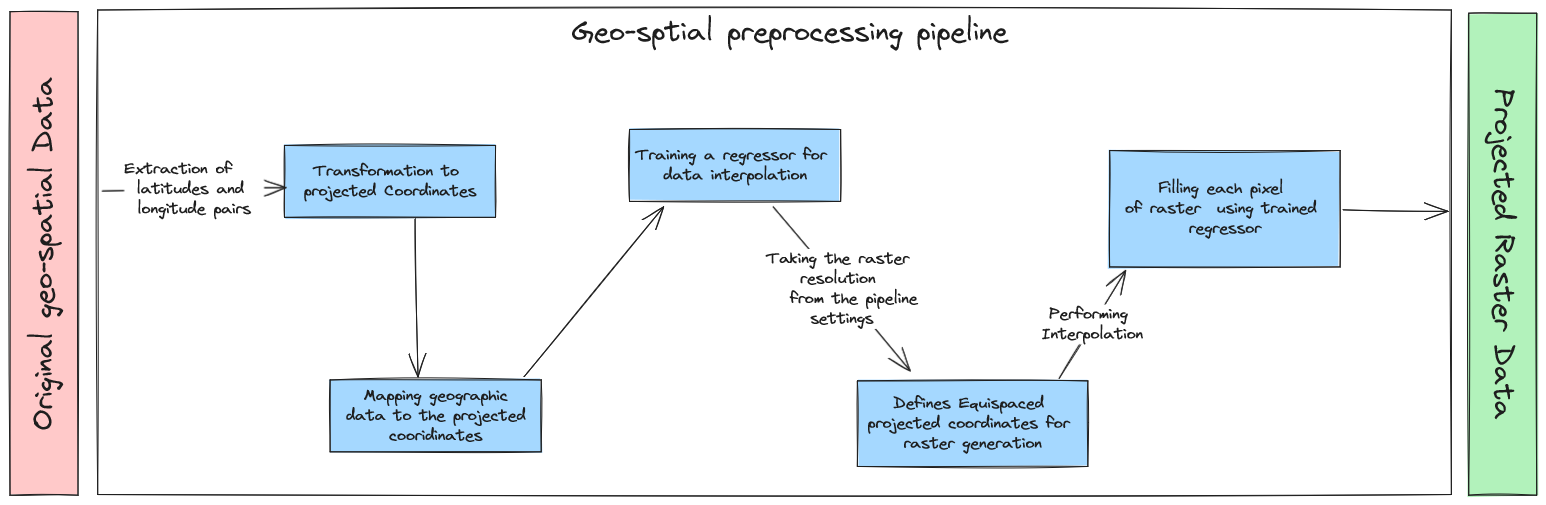
\includegraphics[width=1.0\linewidth]{figures/chapter-7/preprocessing_pipeline.png}
    \caption{geospatial preprocessing pipeline}
    \label{fig:preprocessingpipeline}
\end{figure}
The preceding sections thoroughly explain the geospatial data used to evaluate the convolutions on map projections. In geospatial analysis, the raw data, which maps geo coordinates to the data, cannot be used directly. Scientists commonly employ a preprocessing step to analyze the geospatial data. The data in use, which consists of the monthly observations of geopotential height and precipitation, needs to go through a process and be transformed into a format that could be easily analyzed.

There are two ways to transform the raw data into reduced spatial entities. These reduced spatial entities are classified as Vector or Raster data models, both acceptable by most GIS software.

As our interest is in map projections, the purpose of the preprocessing pipeline is to generate map projection rasters from the raw data. Different Python libraries are utilized for this raster generation. The initial sections of the current chapter explain these tools and libraries.

\section{Data Raster}
\begin{figure}[h]
    \centering
    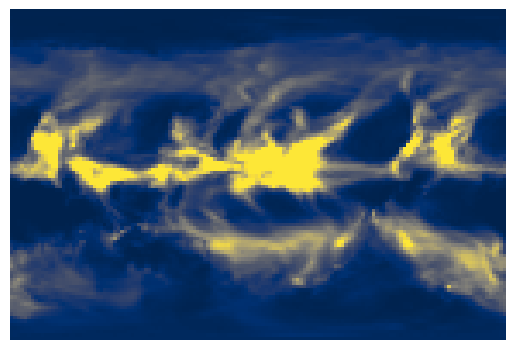
\includegraphics[width=0.75\linewidth]{figures/chapter-7/precipitation_raster_thesis.png}
    \caption{Precipitation raster data with dimensions 96x144}
    \label{fig:precipitation-raster}
\end{figure}
Raster data is employed in the analysis of geographical data. A raster is a grid structure containing data, wherein each cell signifies the data's actual value. The raster's coordinates are determined by its resolution, representing the transformed projected reference system coordinates.


\section{Proj and python's pyproj Package}


\subsection{Proj}
The primary purpose of PROJ is that it is a coordinate transformation
software. It converts the geospatial coordinates from one coordinate reference system (CRS) to another CRS. The software allows transformations to cartographic projection or projected reference systems and geodetic reference systems. The PROJ software provides a command-line interface to interact with its main functionality. The command-line interface can transform from the coordinates provided as user input or files. It also exposes an API to interact programmatically. The ease of usage to interact with the functionality of the PROJ software makes it a popular choice among the different Python libraries and packages that process geospatial data.

"Cartopy" is a popular package for geospatial data visualization. It also uses PROJ when dealing with coordinate reference system transformations. Different data visualization and processing libraries, such as matplotlib, array, and geoPandas, provide interfaces to incorporate Cartopy.

The PROJ software provides an extensive list of map projections. Though the number of map projections in the literature is too great to incorporate into the software, it still provides ample map projections. The software also provides a geodetic transformation facility.

"Reference: taken from PROJ project about page."

\subsection{Proj strings}

Before discussing the Proj strings, it is necessary to discuss the different formats used for storing the information of coordinated reference systems. Multiple formats are used for encoding a coordinate reference system. In light of this thesis, mentioning EPSG codes and WKT is deemed essential to bring discussion to the Proj4 strings.

The primary standard in use is the well-known text WKT. WKT is standardized by the Open Geospatial Consortium (OGC). This format describes the geographic features as standardized text representation. The WKT can represent vector geometry objects, spatial reference systems of spatial objects, and transformations between spatial reference systems (SRS). The significance of WKT lies in its ability to provide a concise and easily understandable representation of various geometric objects, including lines, polygons, triangulated irregular networks (TINs), polyhedrons, and enclosed areas on a map. Furthermore, it serves as a valuable tool for succinctly describing the essential components of coordinate reference system (CRS) definitions, enabling efficient communication and analysis within spatial data. The details for the standard are at \url{"https://docs.ogc.org/is/18-010r11/18-010r11.pdf"}
\begin{lstlisting}
POLYGON ((0 0, 4 0, 4 4, 0 4, 0 0), (1 1, 1 2, 2 2, 2 1, 1 1))
\end{lstlisting}
The European Petroleum Survey Group (EPSG) code is one of the other standards for encoding CRS. EPSG codes are primarily four digits long, but the number of code digits can increase. These codes are specific to only one projected reference system or coordinate systems of different types. The EPSG:4326 describes simple longitude and latitude pairs, which represent the Datum of WGS84.

The Proj.4 strings do incorporate the projected reference system well. The main advantage of using the "Proj.4" strings is that they are human-readable. It is a string that provides different parameters to control the different aspects of the geographic or projected transformation. Here is an example of a "Proj.4" string.

\begin{figure}[h]
    \centering
    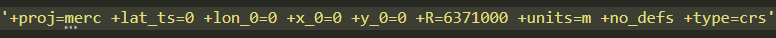
\includegraphics[width=1.0\linewidth]{figures/chapter-7/proj_string_mercator.png}
    \caption{Proj.4 string for Mercator projection}
    \label{fig:proj-string-mercator}
\end{figure}

All the arguments in the "Proj.4" format string start with a plus (+) sign. The values are assigned to the arguments using an equal sign (=), just as one will do when handling the command line arguments with longer names. The most prominent arguments of the string are +proj and +type. The +type argument tells the PROJ software which type of transformation occurs in the string. The type of transformation is between coordinate reference systems. As mentioned in the earlier sections, the projected reference system is a coordinate reference system. The argument +proj tells the name of the projection. The above "Proj.4" string argument has the value of "merc," which indicates transformation happens to  Mercator projection.
\begin{figure}[h]
    \centering
    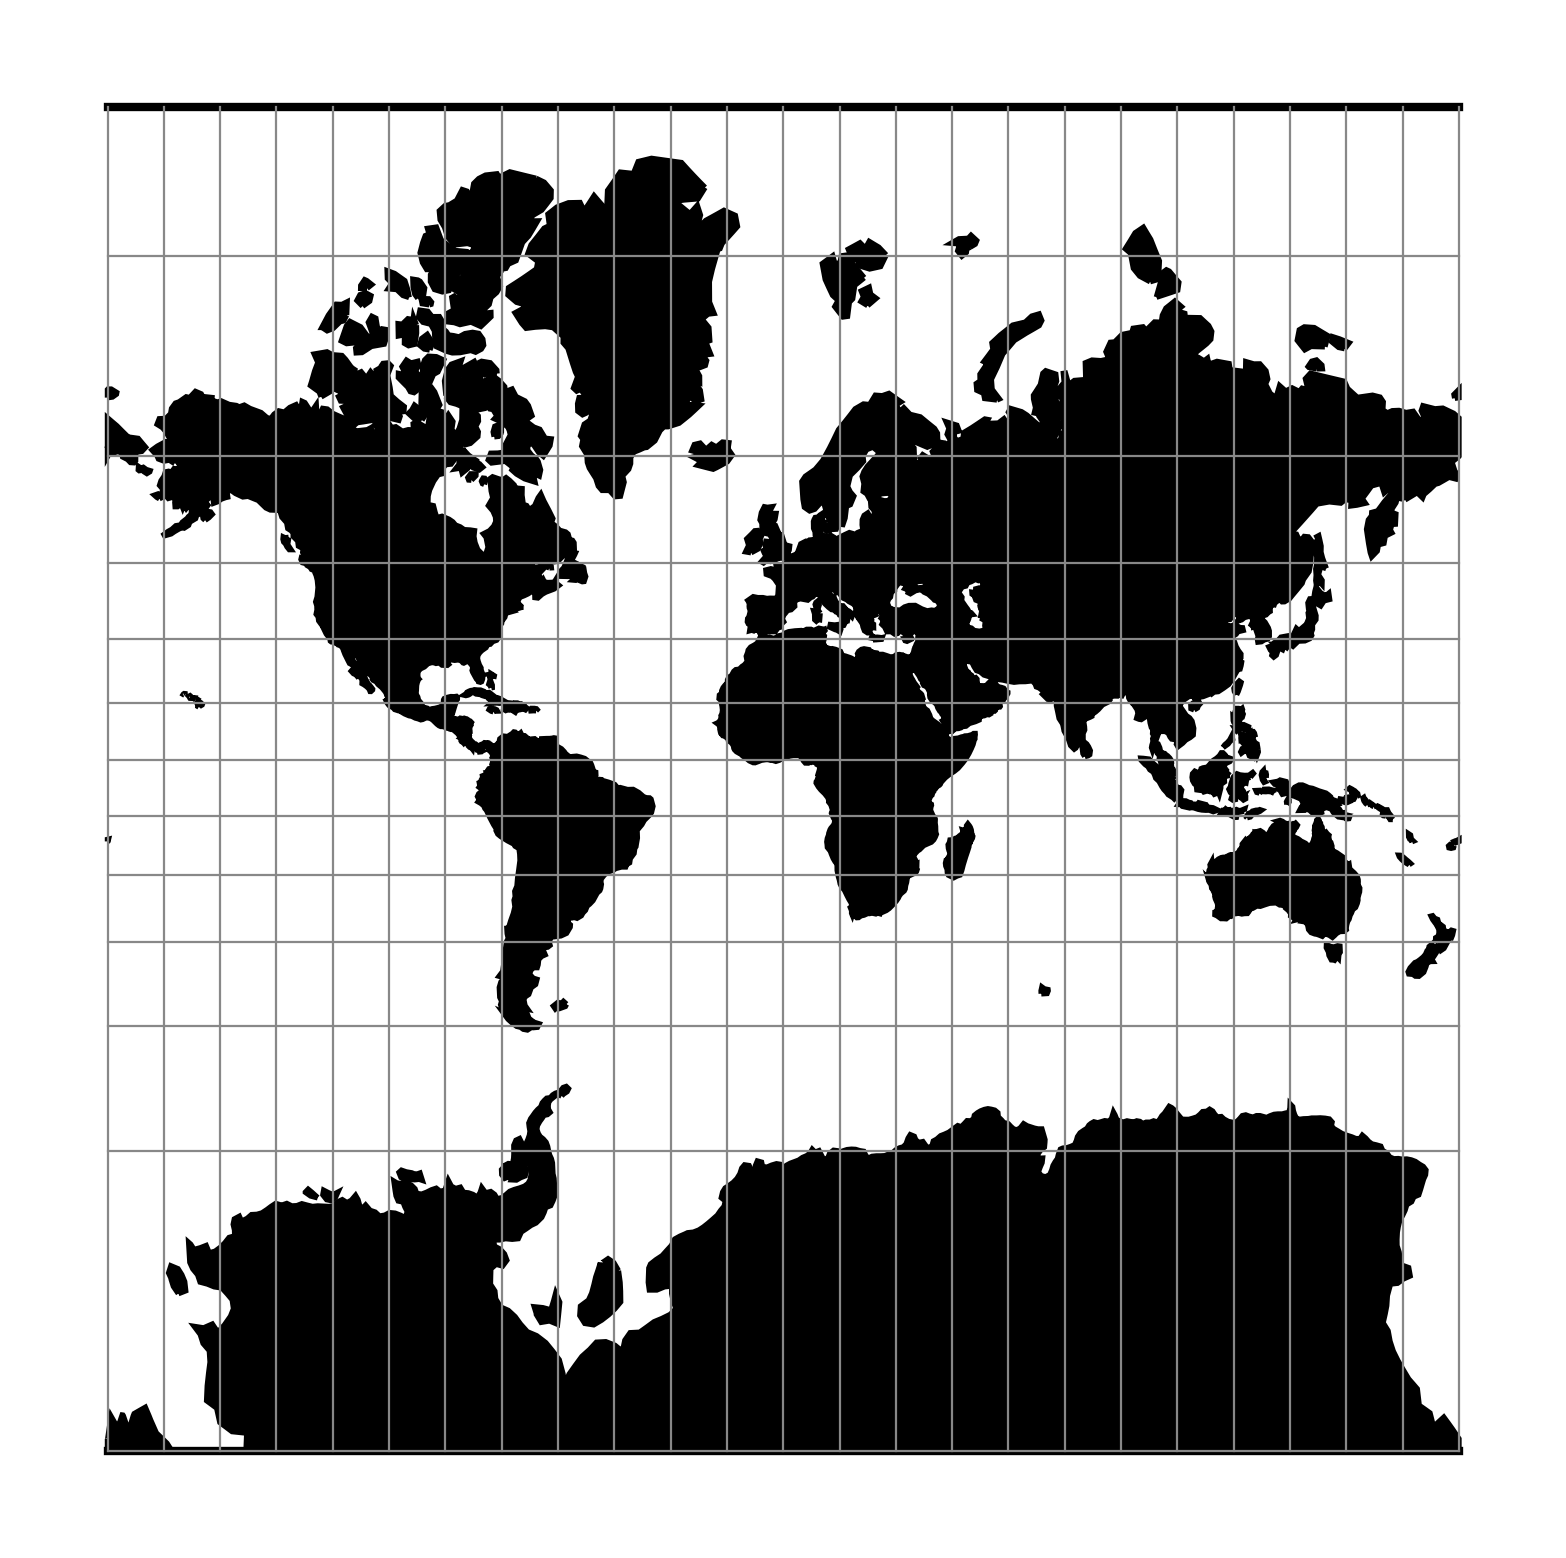
\includegraphics[width=0.5\linewidth]{figures/chapter-7/merc.png}
    \caption{Mercator projection (Source: \cite{PROJ_SITE})}
    \label{fig:mercator-projection}
\end{figure}

This "Proj.4" string transforms the EPSG: 4326 latitude and longitude coordinate pairs to the Mercator projected coordinates.

The advantages of using the "Proj.4" strings for the transformation are as follows:
"Proj.4" format strings are human-friendly and readable. The separation of the arguments for the transformation makes them understandable.
The "Proj.4" format allows us to change the transformation's parameters. Compared to the EPSG codes, which have fixed parameters regardless of whether we consider the projected or geodetic coordinate reference systems, the " Proj. 4 " format allows you to change the transformation's parameters.
Some of the parameters +datum or +R give precise control over the transformation. These parameters are about the ellipsoid used for the transformation.

A complete list of all the shared arguments is in the table below, as some of the projections can have different arguments. Cartographers and geographers can better interpret the arguments.

"https://loc.gov/preservation/digital/formats/fdd/fdd000548.shtml"
"Reference: https://mapscaping.com/a-guide-to-wkt-in-gis/"
\subsection{pyproj}
pyproj is a Python package that is an interface to Proj software. The package provides programming interfaces for using the "Proj.4" strings. Not only to handle the "Proj.4"  CRS format and the newer version, "Proj.5". The "Proj.4" is commonly used for projected reference systems in most GIS systems. The package can handle the EPSG-coded format for CRS as well. The main interface used in the preprocessing pipeline is the "Transformer" class, which takes the argument of the base coordinate reference system and the target projected reference system "Proj.4" string.

\section{Data transformation to projection}
Converting the geographic coordinate reference system is possible solely if the base reference system is provided. Direct conversion from one projected reference system to another is not possible. As mentioned in the chapter introduction, the ultimate goal of the preprocessing pipeline is to generate projected raster data. When the pipeline finishes processing, it generates a raster as the data is in the projected reference system.
It is worth mentioning that the conversion from one projected reference system to another involves a series of transformations.

The series of transformations are as follows:
\begin{itemize}
    \item The pairs of coordinates are in a projected reference system. The projected reference system coordinates will be first transformed to the geographic CRS coordinates.
    \item After the first step, the geographic CRS coordinates are transformed into the desired projected reference system.
\end{itemize}
\begin{figure}[h]
    \centering
    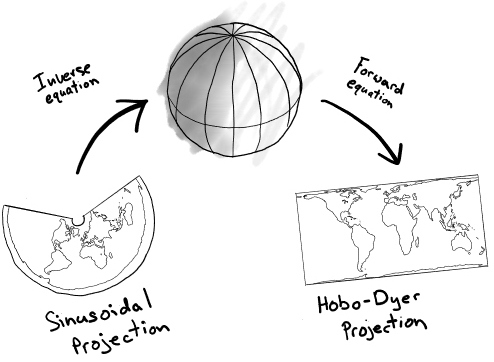
\includegraphics[width=0.5\linewidth]{figures/chapter-7/d_reprojection_example.jpg}
    \caption{transformation between projected reference systems (Source \cite{PROJ_IMAGES})}
    \label{fig:transformation-between-projected-reference-systems}
\end{figure}



Firstly, a CRS is specified for the coordinates that must go through the transformation into a projected reference system. After that, a conversion of the coordinates to the projected reference system is possible. This distinction was necessary because a CRS or a PRS are simply float numbers. The range of the latitudes and longitudes for CRS in ESPG:4326 is from -90 to -90 and 0 to 360, respectively. This base CRS ensures that data for conversion to the projected reference system does not violate the ranges. Otherwise, the underlying PROJ software throws an error regarding the values of the latitudes and longitudes are out of range. The actual value range of the longitudes is from -180 to 180, but PROJ allows the ranges above for the longitudes by radial calculations.\url{https://pygis.io/_images/d_reprojection_example.jpg}

The pyproj package's Transformer class is used to transform the coordinates. The class provides a function "from\_proj" to initialize the Transformer object for performing the transformations. The parameters for the Transformer class are the base CRS and the "Proj.4" string. The base CRS is in the EPSG code, which is 4326, equivalent to the "Proj.4" string "+proj=latlon." This Transformer object is used to create a mapping with the geographical data.

The original data is in a grid shape. The geospatial data chapter explains this property of the data. The conversion happens on a mapping of each latitude and longitude pair. Each pair of coordinates goes through the transformation (via the Transformer object) to the respective projected reference system mentioned in the pipeline settings. This mapping also associates any geographic data with the pairs of transformed coordinates. Thus, it completes the transformation of the latitude and longitude pairs to the projected coordinate reference system and creates the association with the geographical data.


\section{Data Interpolation }
It is common practice to analyze geospatial data by generating data rasters, which can be of any dimension. In our case, the resolution or dimension of the data is 240 by 240. The chapter concerning data explains the dimensions of the original data. If we place the data in the 240 by 240 grid, that data grid would be sparse. A 240 by 240 grid means 57600 data points. The problem then becomes of the form of multivariate regression. Different regression algorithms are used to generate the rasters to overcome the issue of the data's sparsity.The preprocessing pipeline offers two types of regression algorithms.

\begin{itemize}
    \item K-nearest neighbor regression
    \item Gaussian process regeression
\end{itemize}
For the experimentation, K-nearest neighbor regression is trained on the projected coordinates and the geographical data. K-nearest neighbors regression is a method utilized in statistical analysis for predicting continuous numerical values. The advantage of KNN regression is that it processes the data memory efficiently.

The previous section explains the data transformation. The transformation function returns a mapping of the projected coordinates with the geographical data. This mapping is then used for the training of the k-nearest neighbor regressor. This regressor is trained by the hyperparameter of k=10. The machine learning library sklearn is used for the regression algorithms. This step returns a trained regressor, which is used in the further steps for generating the data raster.
\begin{figure}[h]
    \centering
    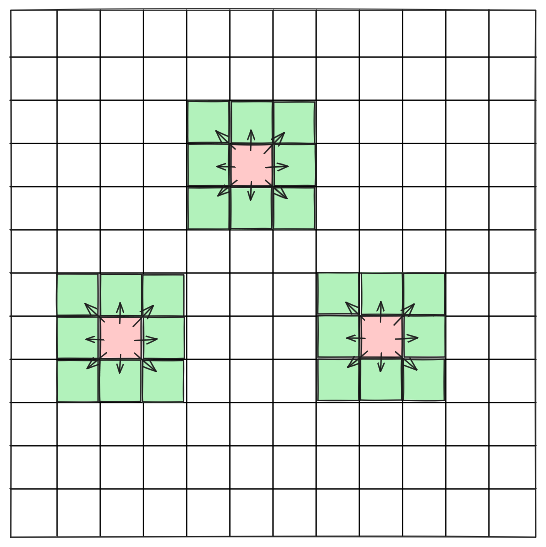
\includegraphics[width=0.5\linewidth]{figures/chapter-7/raster_interpolation.png}
    \caption{K-nearest neighbor learning}
    \label{fig:knn-learning}
\end{figure}

\section{Raster data generation}

Generating the data raster according to the resolution entails a series of steps that utilize the Numpy spline function. The minimum and the maximum of the projected coordinates are calculated. By leveraging this information, it becomes possible to accurately generate equi-spaced projected coordinates that align with the desired resolution of the raster.
The spline function considers the projected coordinates and utilizes them to generate equispaced coordinates. It achieves this by considering the raster's resolution and ensuring that the generated coordinates are distributed in a manner that aligns with the given resolution.
Following this, the trained regressor, specifically the K-nearest neighbor in our case, is utilized to predict the values for the geographical data that will populate the raster. In our scenario, a raster of 240 by 240 was employed. This concludes the process of creating a singular raster.

\section{raster data generation settings}
This section explains the main arguments required to generate the raster data. The first argument of 'projection' takes in an enum value associated with the Proj.4 strings for different projections. The 'regressor\_type' takes the value of which regressor is used. The resolution argument plays an important role in defining the resolution of the raster and the input shape of the convolutional neural network used in the experimentation.
\begin{lstlisting}[language=Python, caption=Pipeline raster data settings]
class PipelineSettings(BaseModel):
    projection: Projections
    regressor_type: RegressorEnum
    resolution: int 
\end{lstlisting}

\section{Raster generation Step}
\begin{algorithm}
    \caption{Preprocessing steps}
    \label{}
    \begin{algorithmic}[1]
        \FOR{ each data point in the list given to the preprocessing pipeline}
        \STATE Extracts the Latitudes and Longitudes for each data point
        \STATE Creates a Transformer object for the coordinates transformation
        \STATE Generates a mapping of the geographical data with the projected coordinates
        \STATE Trains a regression model from mapping with projected coordinates and geographical data
        \STATE Extracts the minimum and maximum values of the projected coordinates
        \STATE Generates the equispaced arrays from the minimum and maximum values of the coordinates using NumPy's spline
        \STATE Predicts the values to fill the raster using the mappings of the newly generated equispaced coordinates  using the trained regression model

        \ENDFOR
        \STATE Returns the data raster list
    \end{algorithmic}
\end{algorithm}

\clearpage
\cleardoublepage

\chapter{Approach}
\label{chap:approach}
In  \autoref{chap:related_work} I discussed different architectures and convolutions on non-Euclidean spaces, specifically spherical CNN which brings closer the
representation of geospatial data closer to the actual representation of the Earth. Regardless of the advances being done in the geometric machine learning,
most of the GIS systems are in use of map projections for geospatial data for the analysis. In particular, specific types of map projections are only used for
the analysis of the geospatial data in the GIS systems. The GIS systems are only focusing on cylindrical projections and over looking the errors generated by
the distorted projections. Even though there are numerous projections in the literature, a thorough investigation of the different types of map projections is still
needed which could bring out the potential for the representation of the geospatial data on the global level. Map projections employ an approximation of the true form
of the geoid using an ellipsoid. This has motivated our investigation into the different types of map projections for geospatial analysis.

\begin{figure}[h]
    \centering
    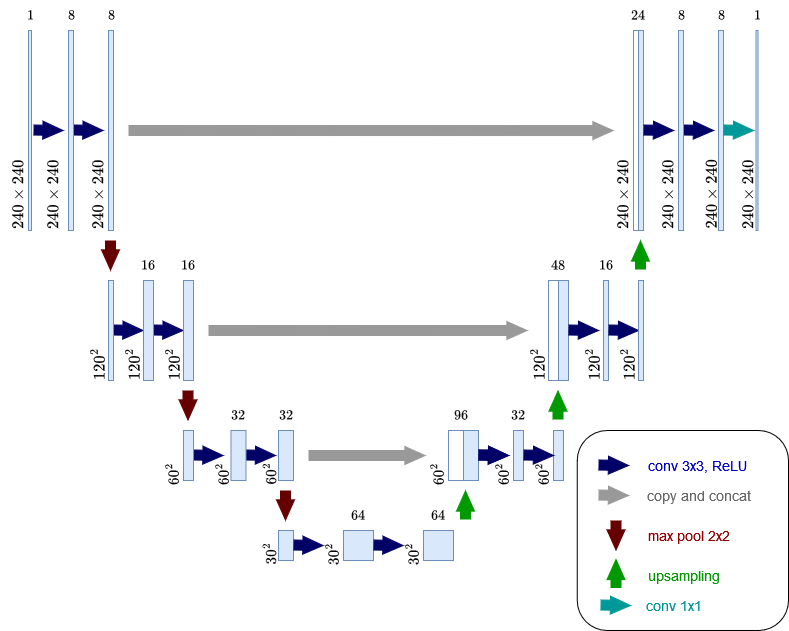
\includegraphics[width=1.0\linewidth]{figures/chapter-5/my_unet.png}
    \caption{U-Net architecture for experimentation }
    \label{fig:self-unet}
\end{figure}

Map projections are planer in nature, to capture the spatial correlation on the projected geospatial data, I utilized the power of convolutional neural networks.
In specific I used the U-NET \cite{ronneberger2015unet}  based architecture to understand the effects on 2D convolutions following \cite{trebing2021smaatunet}, to generate projected precipitation data on the global scale by giving the geopotential height projected data as input to the U-Net model.

\section{Architecture}
For this purpose, I defined a shallow U-Net \textbf{architecture}, with four contraction blocks which contains two convolutional layers with rectified linear unit (\textbf{ReLU})
as activation function, with zero-padding and kernel of size (\textbf{3x3}), for contracting the feature maps max pooling layer with pool size (\textbf{2x2}) is used after the two
convolutional layers.
After the contraction blocks the expansion block are introduced in the architecture with up sampling layers with \textbf{interpolation} strategy of the nearest neighbors is used
and followed by two convolutional layers with same settings as in the contracting path of the model.
The last layer in which the network is generating the map projected precipitation rasters, a 2D convolutional layer is used by kernel size  \textbf{(1x1)}.

The main feature in the U-Net architecture is that the feature maps from the encoder part of the model (left hand side) shown in the figure ~\ref{fig:self-unet} are concatenated to the decoder part of the model (right hand side).
This concatenation enhances the reconstruction of the output by joining the hierarchically learned features at each encoder's convolutional block of the network. This could be
understood as the convolutional neural networks make sense of the features in an hierarchical manner by passing feature maps and performing convolutions at deeper levels,
learning the primitive features at the upper level and learning the fine grained features are the deeper level. The reconstruction of the precipitation raster in the decoder
part happens in a bottom up fashion facilitated by the concatenation of the features maps of the encoder part of the network. Figure ~\ref{fig:self-unet} depicts the complete architecture.

\section{Hyper Parameters}
\begin{itemize}
    \item The learning rate for the training of the loss function is $\eta = 0.001$, the learning rate was kept same for all the experiments regarding different map projection types to see only the effects of the convolutions on the map projections.
    \item \textbf{Adam optimization} is used for the boosting the training of the model.
\end{itemize}

\begin{figure}[h]
    \centering
    \begin{minipage}{0.45\textwidth}
        \centering
        \includegraphics[width=0.9\linewidth]{figures/chapter-5/plate_caree_geopoth_raster.png}
        \caption{ Geopotential height raster data as Plate-Carrée projection}
        \label{fig:plate_geopoth_raster}
    \end{minipage}\hfill
    \begin{minipage}{0.45\textwidth}
        \centering
        \includegraphics[width=0.9\linewidth]{figures/chapter-5/plate_caree_prect_raster.png}
        \caption{Precipitation raster data as Plate-Carrée projection}
        \label{fig:plate_prect_raster}
    \end{minipage}\hfill
\end{figure}

\newpage

\section{Training Process}

For the setting of our experiments, I considered the prediction of the precipitation on the global level on the basis of geopotential height as a regression problem. For this reason I selected mean squared error (MSE) as a loss function for training the model.

Mean Squared Error is defined as:

\begin{gather*}
    MSE = \dfrac{1}{n}\sum_{1 = 1}^{n}(Y_i-\hat{Y}_i )^2
\end{gather*}

The training process of models is depending on the preprocessing of the geospatial data, where the original data is converted to rasters. For our experiments, I have created the raster of (240x240) rasters as mention in chapter \ref{chap:preprocess}. The reason to select the specific resolution of the raster is to have more data on the latitudes axis because the original data had lesser dimension on the latitude axis as mentioned in chapter \ref{chap:dataset}.
I am considering only a single type of geospatial data such as (geopotential height or precipitation), so the input data given to the network has a single channel,  the \textbf{input size} is $(1 \times 240  \times 240)$ for the network.
The output of the network is a precipitation raster, with the dimension same as the input dimension $(1 \times 240  \times 240)$. The data is splitted in three folds, making training set, validation set and the test set.

The total number of \textbf{trainable parameters} of the network are \textbf{122473}.
\section{Evaluation Metrics}

To evaluate the models I am not only looking at the training loss and validation loss for just looking at how well the model is being trained but I am measuring mean absolute error metric for the evaluation of the regression problem.
\begin{itemize}
    \item \textbf{Mean Absolute Error}\\
          \begin{gather*}
              MAE = \frac{\sum_{1 = 1}^{n}\left\lvert
                  y_i - x_i
                  \right\rvert}{n}
          \end{gather*}

          where $y_i$ is the predicted value and $x_i$ is the true against which the metric value is being measured. In this case I will be comparing the predicted precipitation raster with the original precipitation raster.
\end{itemize}


\clearpage
\cleardoublepage

\chapter{Experiments \& Results}

\label{chap:experiments_results}

In this chapter, I will analyze the outcomes of our extensive experimentation with various map projections and their impact on the performance
of Convolutional Neural Networks (CNNs), specifically focusing on the U-Net architecture. By systematically applying these models to various types of
map projections. I aim to clarify the subtle impacts these projections have on the accuracy and efficiency of
geospatial data analysis. This inquiry is rooted in a comprehensive experimental structure devised to evaluate the model's capacity to forecast precipitation patterns
from geospatial data inputs, thereby furnishing valuable insights into the optimal utilization of CNNs in the realm of geospatial analysis.

% Through this section,
% I strive to bridge the divide between theoretical knowledge and practical implementation, making a significant contribution to the advancement of the field by
% highlighting potential avenues for future research.

% The experimentation is conducted on four different types of map projections, namely Cylindrical, Pseudocylindrical, Conic and Planar projections.
% Then I have selected four map projections in each of the main projection types.
% The U-Net model mentioned in \autoref{chap:approach} is trained for 20 epochs for each of the map projections. Initially 120 epochs were defined for the experimentation, for each of the models the phenomenon of overfitting started to occur over the training period, to mitigate the issue \textbf{early stopping} was deployed and each model was trained for 20 epochs.
% Mean absolute error (MAE) is used as a metric for the evaluation of the model.

% 16 geospatial raster datasets with the raster resolution of 240x240 were generated for the experimentation, via the process of creating rasters as mentioned in \autoref{chap:preprocess}. The loss and the metrics discussed in the result section are the average results, as for each map projection dataset the U-Net model is trained four times mitigating the issue of randomness in the network's parameters.

% The training of the models is displayed for all of the 4 cylindrical projections and 3 of the pseudocylindrical projections, and the values of the metrics used for the evaluation of the model is displayed in a tabular form.
% For the conic and the planar projections only the evaluation metrics are shown. In the end I will discuss the overall map projections.

\section{Experimental Setup}
The experimentation is carried out on a total of four distinct types of map projections, specifically Cylindrical, Pseudocylindrical, Conic, and Planar projections.
To ensure comprehensive coverage, I have carefully chosen four map projections within each of these main projection types, these projections are chosen on the distortions that these projections are trying to preserve.

\subsection{Early Stopping}
The U-Net model, as mentioned in \autoref{chap:approach}, undergoes a training process comprising 20 epochs for each of the map projections.
Originally, a total of 120 epochs were designated for the experimentation; however, it became apparent that the phenomenon of overfitting occurred throughout the
training period for each of the models. To address this challenge, the strategy of "early stopping" was deployed, resulting in the training of each model for a reduced
duration of 20 epochs.

\subsection{Performance Evaluation}
In order to evaluate the performance of the U-Net model, the mean absolute error (MAE) is employed as a metric. This metric serves as a reliable measure to gauge
the accuracy and precision of the model's predictions.
\subsection{Raster Generation}
Furthermore, a set of 32 geospatial raster datasets (each with a raster resolution of 240x240) were generated specifically for the purpose of these experiments, 16 geopotential height map projected rasters datasets and 16 precipitation map projected rasters datasets.
These datasets were created using the raster creation process detailed in \autoref{chap:preprocess}.
It is important to note that the reported loss and metrics discussed
in the results section represent average values. This is due to the fact that for each map projection dataset, the U-Net model is trained four times, thereby mitigating
the potential impact of random variations in the network's parameters. All the results and values are averaged out.
\subsection{Model Training Analysis}
The training progress of the models is meticulously documented for all four cylindrical projections, three of the pseudocylindrical projections.
Additionally, the values of the evaluation metrics employed to assess the model's performance are presented in a concise tabular format.

However, for the conic and planar projections, only the evaluation metrics are showcased as these particular projections do not undergo the same level of detailed training
analysis.

Finally, following the presentation of the specific experimental results, a comprehensive discussion will be conducted to provide an overarching analysis of the
various map projections under consideration.

\clearpage

\section{Cylindrical Projections}

The four cylindrical map projections used for the experimentation are
\begin{itemize}
    \item Mercator
    \item Plate Carree
    \item Cylindrical Equal Area
    \item General Oblique Transformation
\end{itemize}
The selection of the map projections is done based on the underlying properties of the cylindrical map projections mentioned in the \autoref{section:map_projections}. These projections try to mitigate some of the underlying distortions generated by the projections.

\subsection{Mercator}
\begin{figure}[H]
    \centering
    \begin{minipage}{0.30\textwidth}
        \centering
        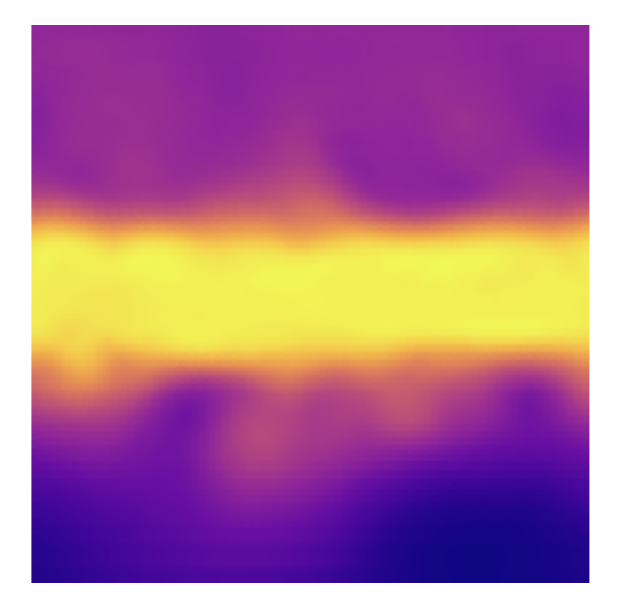
\includegraphics[width=0.9\linewidth]{figures/chapter-8/geopoth_mercator.png}
        \caption{ Geopotential height raster data as Mercator projected}
        \label{fig:merc_geopoth_raster}
    \end{minipage}\hfill
    \begin{minipage}{0.30\textwidth}
        \centering
        \includegraphics[width=0.9\linewidth]{figures/chapter-8/merc.png}
        \caption{Mercator Projection (Source \cite{PROJ_SITE})}
        \label{fig:merc_proj}
    \end{minipage}\hfill
    \begin{minipage}{0.30\textwidth}
        \centering
        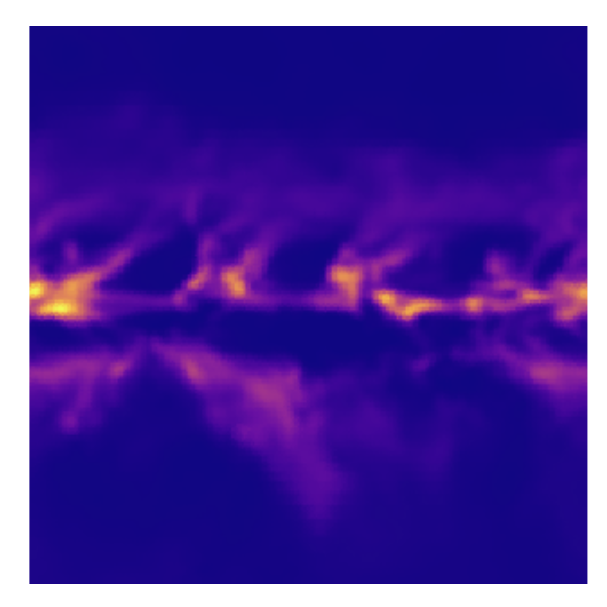
\includegraphics[width=0.9\linewidth]{figures/chapter-8/prect_mercator.png}
        \caption{Precipitation raster data as Mercator projected}
        \label{fig:merc_prect_raster}
    \end{minipage}\hfill
\end{figure}

\begin{figure}[H]
    \centering
    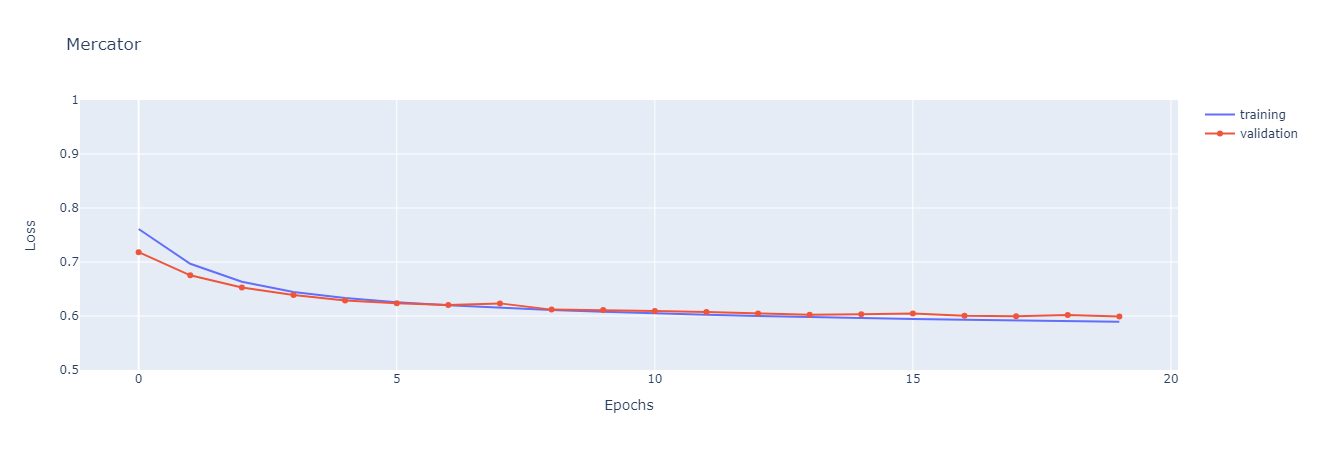
\includegraphics[width=1.0\linewidth]{figures/chapter-8/merc_loss.png}
    \caption{Mercator: Averaged training loss of models  }
    \label{fig:merc_loss}
\end{figure}

\newpage

\subsection{Plate Carree}

\begin{figure}[H]
    \centering
    \begin{minipage}{0.30\textwidth}
        \centering
        \includegraphics[width=0.9\linewidth]{figures/chapter-8/plate_caree_geopoth_raster.png}
        \caption{ Geopotential height raster data as Plate Carree projected}
        \label{fig:eqc_geopoth_raster}
    \end{minipage}\hfill
    \begin{minipage}{0.30\textwidth}
        \centering
        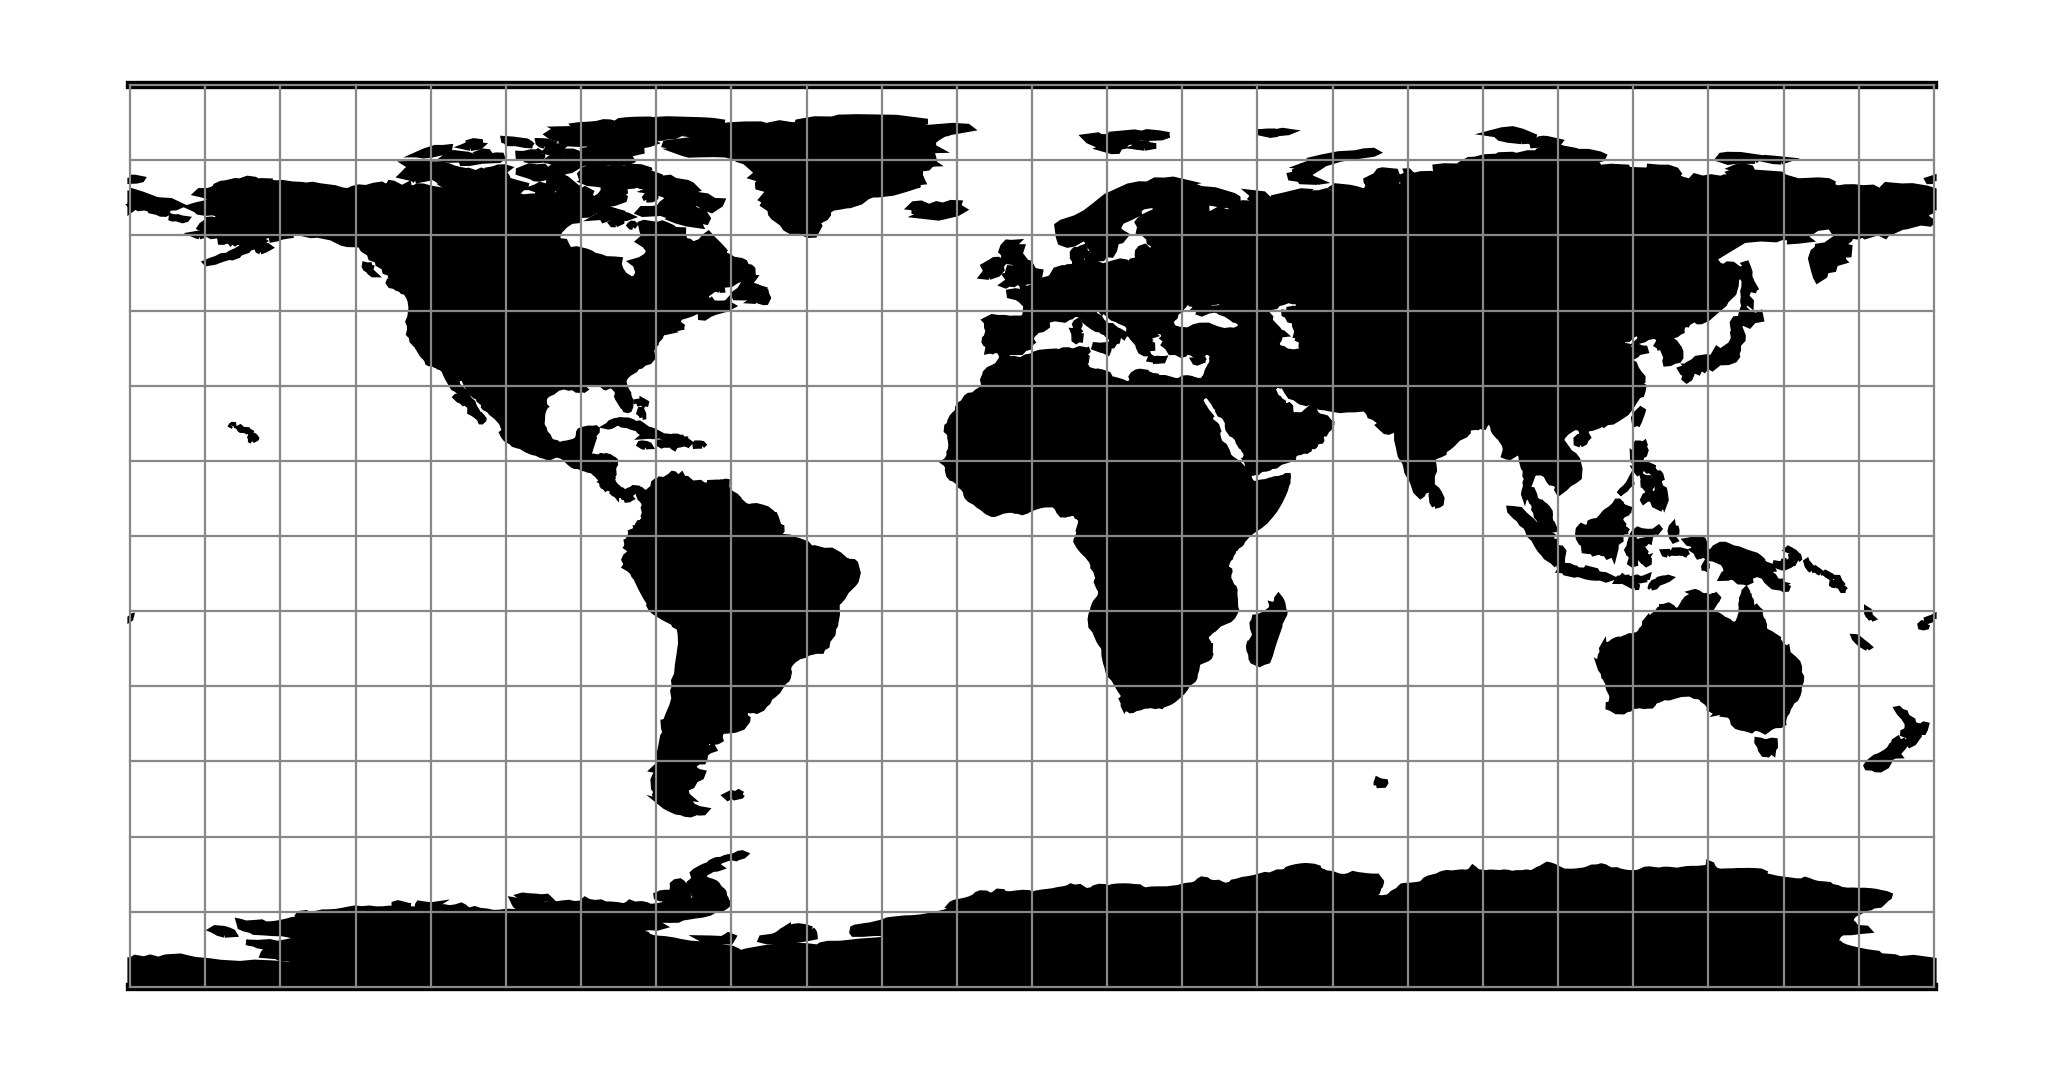
\includegraphics[width=0.9\linewidth]{figures/chapter-8/eqc.png}
        \caption{Plate Carree Projection (Source \cite{PROJ_SITE})}
        \label{fig:eqc_prect_raster}
    \end{minipage}\hfill
    \begin{minipage}{0.30\textwidth}
        \centering
        \includegraphics[width=0.9\linewidth]{figures/chapter-8/plate_caree_prect_raster.png}
        \caption{Precipitation raster data as Plate Carree projected}
        \label{fig:eqc_prect_raster}
    \end{minipage}\hfill
\end{figure}

\begin{figure}[H]
    \centering
    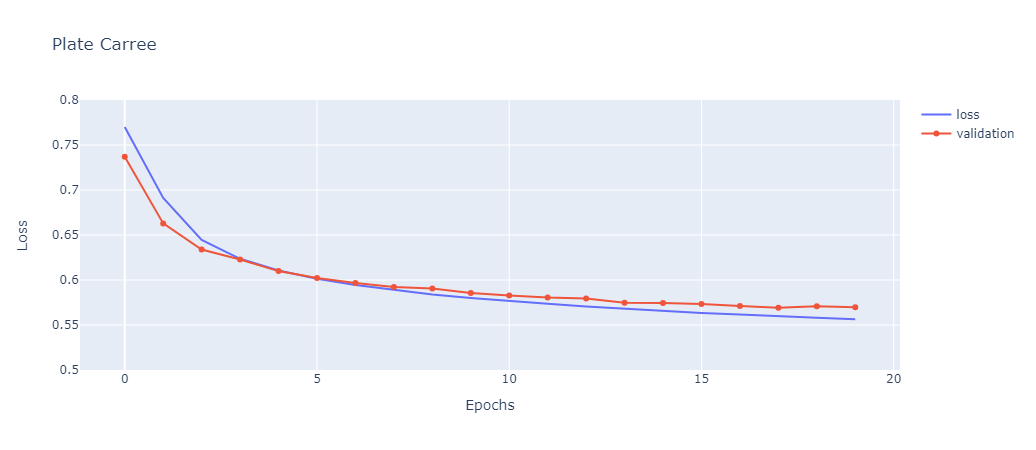
\includegraphics[width=1.0\linewidth]{figures/chapter-8/pc_loss.png}
    \caption{Plate Carree: Averaged training loss of models  }
    \label{fig:pc_loss}
\end{figure}

The trend for the training of the model


\subsection{Cylindrical Equal Area}

\begin{figure}[H]
    \centering
    \begin{minipage}{0.30\textwidth}
        \centering
        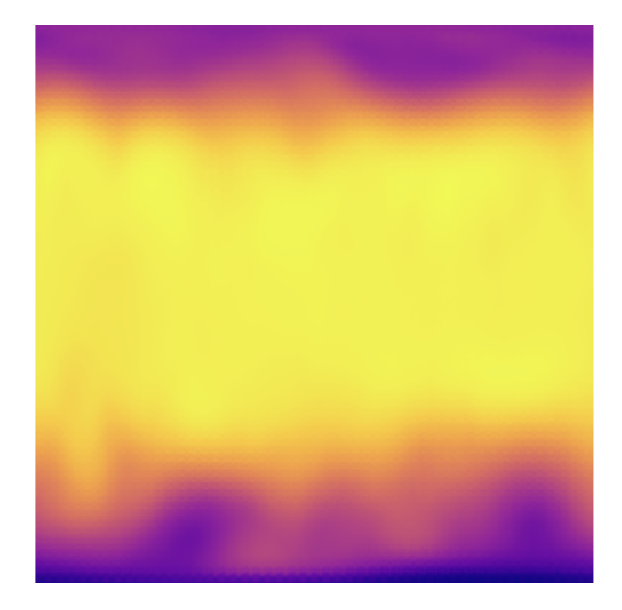
\includegraphics[width=0.9\linewidth]{figures/chapter-8/prect_cea.png}
        \caption{ Geopotential height raster data as Cylindrical Equal Area projected}
        \label{fig:cea_geopoth_raster}
    \end{minipage}\hfill
    \begin{minipage}{0.30\textwidth}
        \centering
        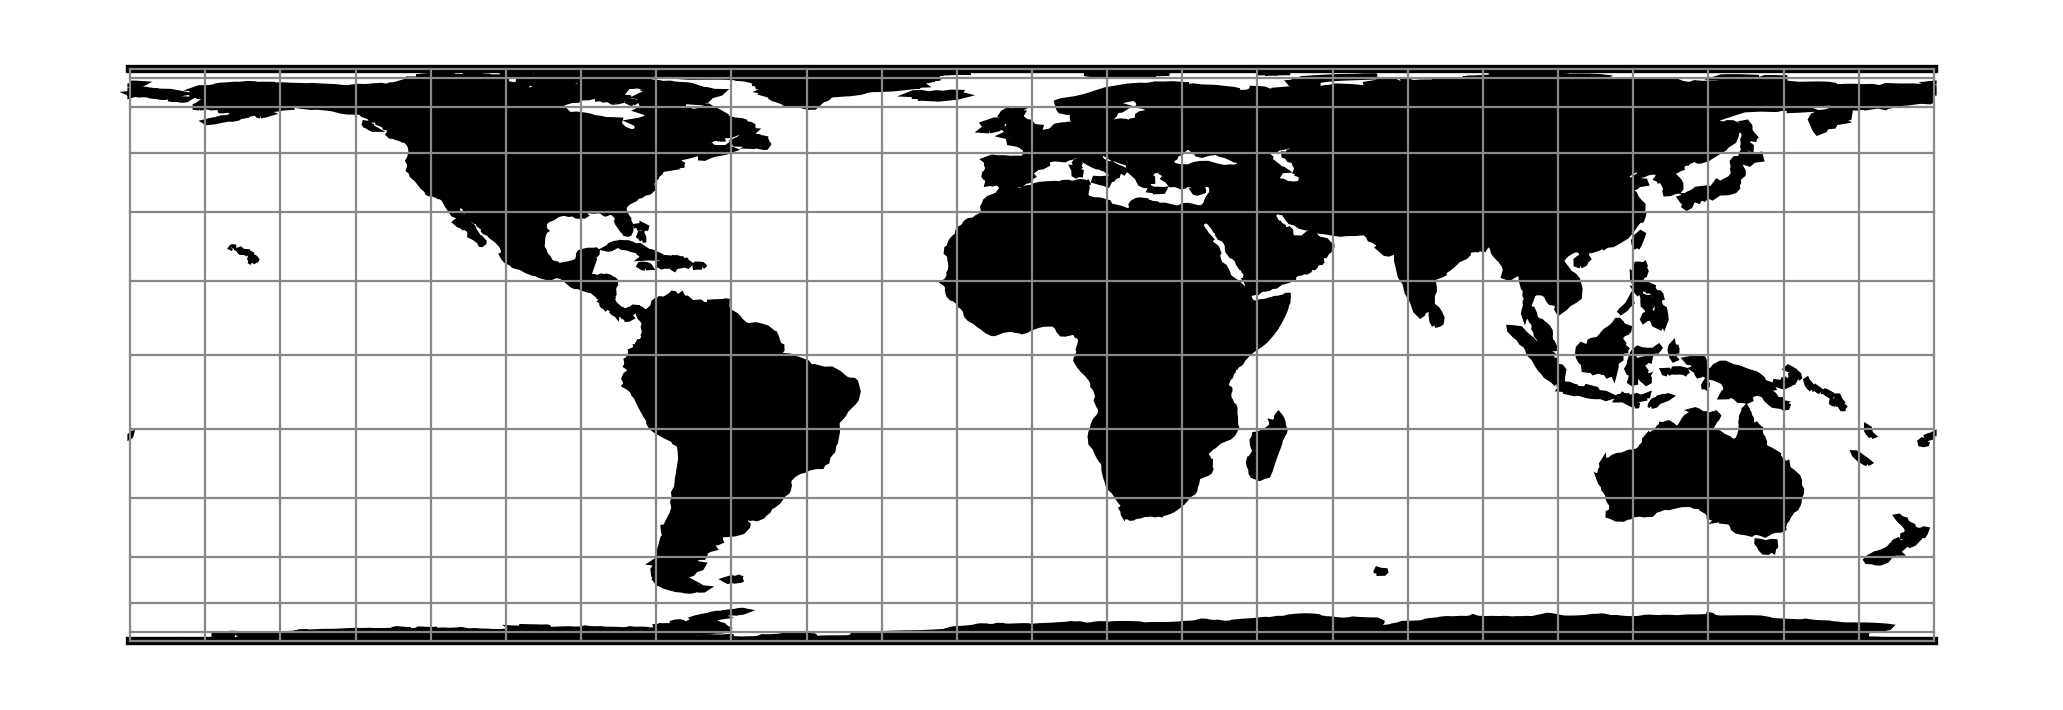
\includegraphics[width=0.9\linewidth]{figures/chapter-8/cea.png}
        \caption{Cylindrical Equal Area Projection (Source \cite{PROJ_SITE})}
        \label{fig:cea_prect_raster}
    \end{minipage}\hfill
    \begin{minipage}{0.30\textwidth}
        \centering
        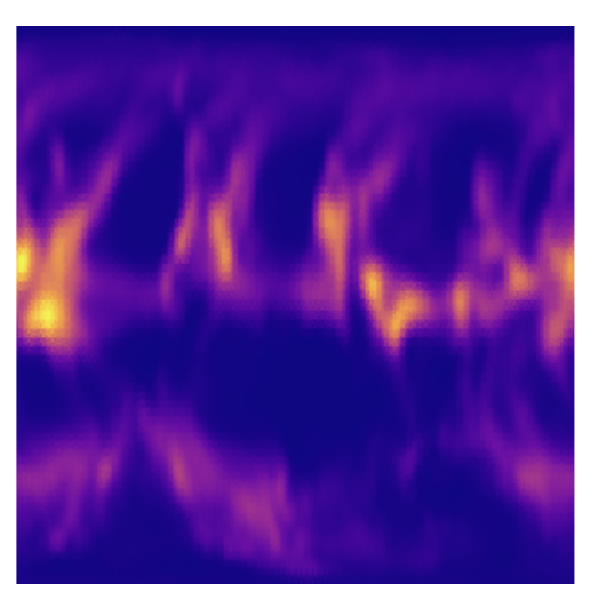
\includegraphics[width=0.9\linewidth]{figures/chapter-8/geopoth_cea.png}
        \caption{Precipitation raster data as Cylindrical Equal Area projected}
        \label{fig:cea_prect_raster}
    \end{minipage}\hfill
\end{figure}

\begin{figure}[h]
    \centering
    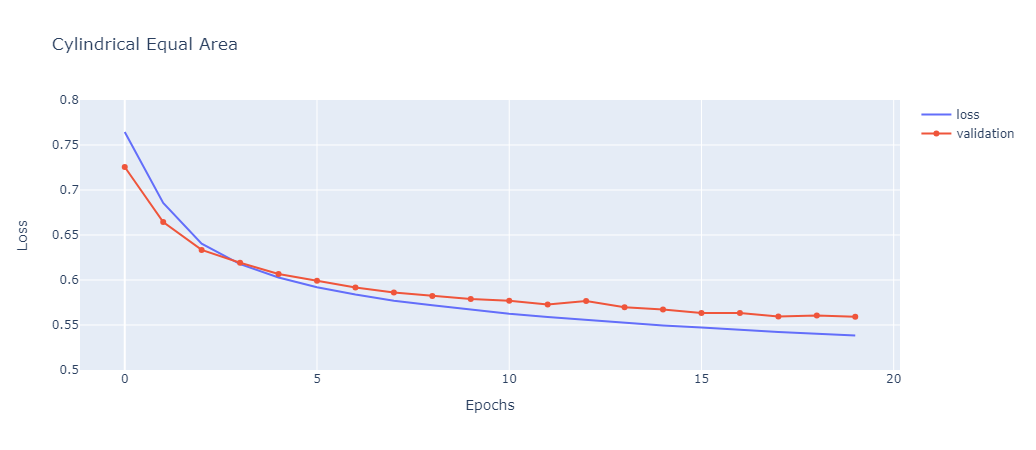
\includegraphics[width=1.0\linewidth]{figures/chapter-8/cea_loss.png}
    \caption{Cylindrical Equal Area: Averaged training loss of models  }
    \label{fig:cea_loss}
\end{figure}

\subsection{General Oblique Transformation}
\begin{figure}[H]
    \centering
    \begin{minipage}{0.30\textwidth}
        \centering
        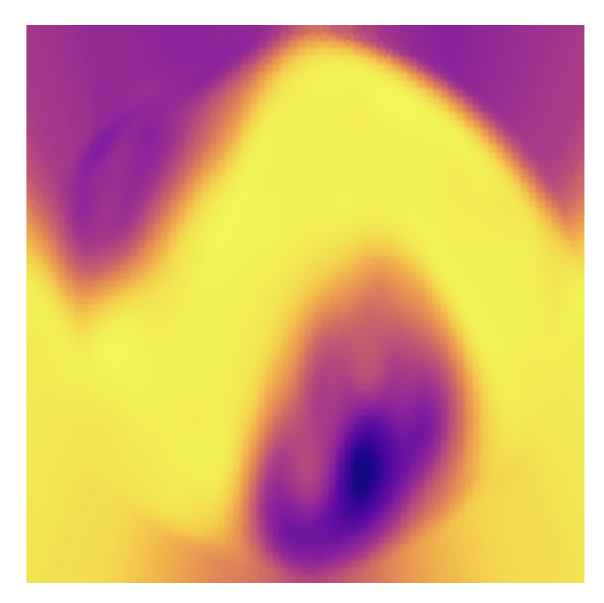
\includegraphics[width=0.9\linewidth]{figures/chapter-8/geopoth_got.png}
        \caption{ Geopotential height raster data as General Oblique Transformation projected}
        \label{fig:ob_tran_geopoth_raster}
    \end{minipage}\hfill
    \begin{minipage}{0.30\textwidth}
        \centering
        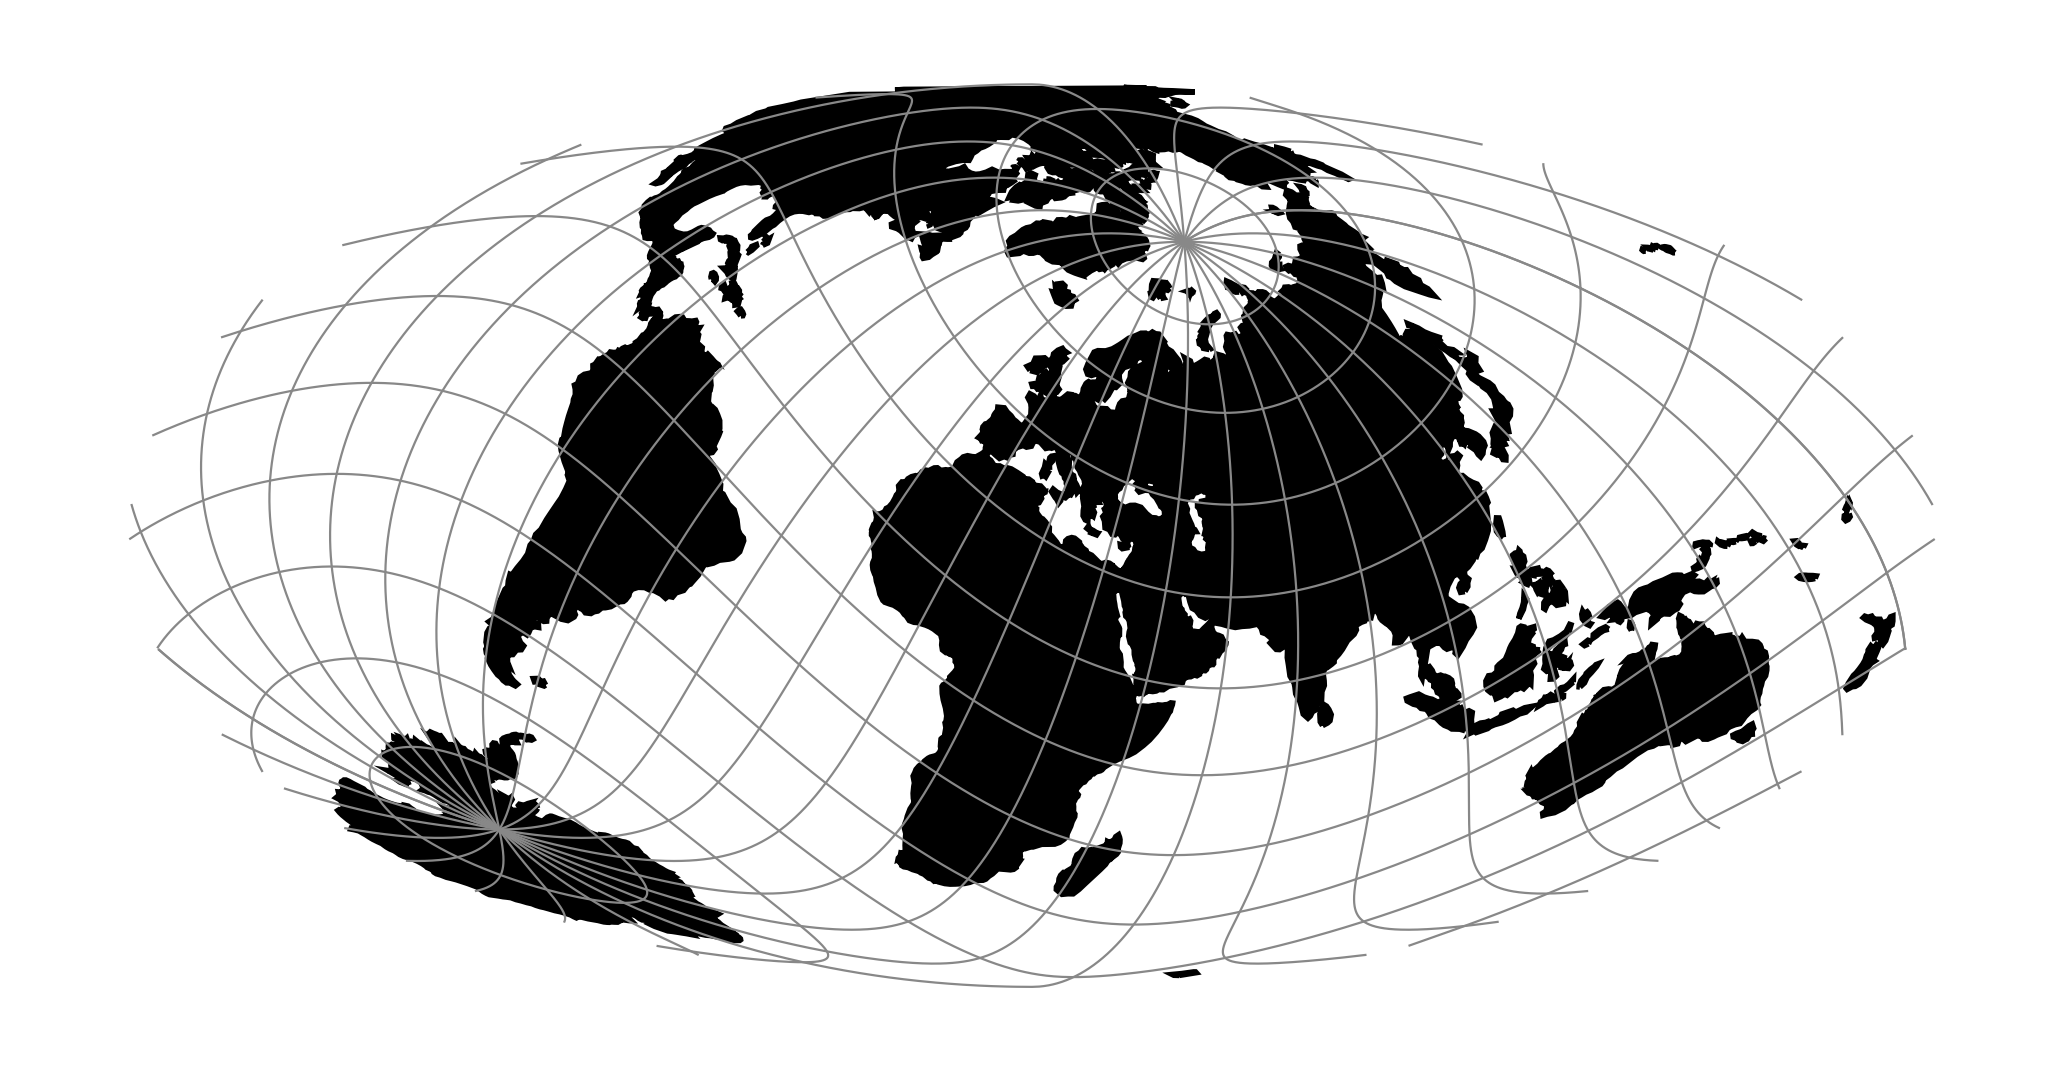
\includegraphics[width=0.9\linewidth]{figures/chapter-8/ob_tran.png}
        \caption{General Oblique Transformation Projection (Source \cite{PROJ_SITE})}
        \label{fig:ob_tran_proj}
    \end{minipage}\hfill
    \begin{minipage}{0.30\textwidth}
        \centering
        \includegraphics[width=0.9\linewidth]{figures/chapter-8/prect_got.png}
        \caption{Precipitation raster data as General Oblique Transformation projected}
        \label{fig:ob_tran_prect_raster}
    \end{minipage}\hfill
\end{figure}

\begin{figure}[H]
    \centering
    \includegraphics[width=1.0\linewidth]{figures/chapter-8/got_loss.png}
    \caption{General Oblique Transformation: Averaged training loss of models  }
    \label{fig:got_loss}
\end{figure}
\subsection{Results \& Observations}
\begin{itemize}
    \item The ~\ref{fig:merc_loss} shows the average training loss for the U-Net model mentioned in the \autoref{chap:approach}, it could be seen that model's training loss is stabalizing and the trend of the validation loss is on a decrease.
          The model is being trained well for the Mercator projection, we need to consider the fact that we have trained a shallow model with less numbers of filters.
    \item The ~\ref{fig:pc_loss} shows the average training loss decreasing and the trend of the validation loss is on an increase after the 17th epoch, with more training the model is on the path to overfit. Early stopping should have been used earlier for this projection dataset.
    \item ~\ref{fig:cea_loss} depicts that the model in training is subjected to overfit very quickly in the training process. Just after the 7th epoch the model is overfitting.
    \item ~\ref{fig:got_loss} shows, the model start to overfit from the 5th epoch.
    \item As soon as the rasters which are generated to resolve some of the distortions occuring due to map projections the rasters.
          The cylindrical equal area projection does resolve the distortion of area but is not able to perform well during the training of the model under observation.
          Same is the case with oblique general transformation projection, as it brings the north polar region at the central level part, but brings huge distortions equator regions.
    \item In our case the input data to the model, geopotential height when subjected to the whole raster, the model in under consideration tends to overfit.
    \item The ~\ref{cylindrical_results_table} depicts the MAE to measure the quality of the predictions of the precipitation on the average results.

\end{itemize}
\begin{table}[ht]
    \centering
    \caption{Summary of Cylindrical Projection Model Performance}
    \label{cylindrical_results_table}
    \renewcommand{\arraystretch}{1.2} % Adjusts the row height
    \begin{tabular}{|l|c|c|c|c|c|}
        \hline
        \rowcolor[gray]{0.9}
        \textbf{\emph{Project Name}}   & \textbf{\emph{Epochs}} & \textbf{\emph{MAE}} & \textbf{\emph{Validation MAE}} \\ \hline
        Mercator                       & 20                     & 0.51                & 0.51                           \\ \hline
        Plate Carree                   & 20                     & 0.49                & 0.49                           \\ \hline
        Cylindrical Equal Area         & 20                     & 0.48                & 0.49                           \\ \hline
        General Oblique Transformation & 20                     & 0.48                & 0.49                           \\ \hline
    \end{tabular}


\end{table}
\clearpage
\newpage

\section{Experiments: Pseudocylindrical projections}
The selected pseudocylindrical projections for the experimentation are mentioned below:
\begin{itemize}
    \item Robinson
    \item Interrupted Goode Homolosine
    \item Sinusoidal (Sanson Flamsteed)
    \item Loximuthal
\end{itemize}
\subsection{Robinson}
\begin{figure}[H]
    \centering
    \begin{minipage}{0.30\textwidth}
        \centering
        \includegraphics[width=0.9\linewidth]{figures/chapter-8/geopoth_robin.png}
        \caption{ Geopotential height raster data as Robinson projected}
        \label{fig:robin_geopoth_raster}
    \end{minipage}\hfill
    \begin{minipage}{0.30\textwidth}
        \centering
        \includegraphics[width=0.9\linewidth]{figures/chapter-8/robin.png}
        \caption{Robinson (Source \cite{PROJ_SITE})}
        \label{fig:robin_proj}
    \end{minipage}\hfill
    \begin{minipage}{0.30\textwidth}
        \centering
        \includegraphics[width=0.9\linewidth]{figures/chapter-8/prect_robin.png}
        \caption{Precipitation raster data as Robinson projected}
        \label{fig:robin_prect_raster}
    \end{minipage}\hfill
\end{figure}
\begin{figure}[H]
    \centering
    \includegraphics[width=1.0\linewidth]{figures/chapter-8/robin_loss.png}
    \caption{Robinson: Averaged training loss of models  }
    \label{fig:robin_loss}
\end{figure}
\subsection{Interrupted Goode Homolosine}
\begin{figure}[H]
    \centering
    \begin{minipage}{0.30\textwidth}
        \centering
        \includegraphics[width=0.9\linewidth]{figures/chapter-8/geopoth_goode.png}
        \caption{ Geopotential height raster data as Interrupted Goode Homolosine projected}
        \label{fig:ig_geopoth_raster}
    \end{minipage}\hfill
    \begin{minipage}{0.30\textwidth}
        \centering
        \includegraphics[width=0.9\linewidth]{figures/chapter-8/igh.png}
        \caption{Interrupted Goode Homolosine (Source \cite{PROJ_SITE})}
        \label{fig:ig_proj}
    \end{minipage}\hfill
    \begin{minipage}{0.30\textwidth}
        \centering
        \includegraphics[width=0.9\linewidth]{figures/chapter-8/prect_goode.png}
        \caption{Precipitation raster data as Interrupted Goode Homolosine projected}
        \label{fig:ig_prect_raster}
    \end{minipage}\hfill
\end{figure}

\begin{figure}[H]
    \centering
    \includegraphics[width=1.0\linewidth]{figures/chapter-8/goode_loss.png}
    \caption{Interrupted Goode Homolosine: Averaged training loss of models  }
    \label{fig:goode_loss}
\end{figure}
\subsection{Sinusoidal (Sanson Flamsteed)}
\begin{figure}[H]
    \centering
    \begin{minipage}{0.30\textwidth}
        \centering
        \includegraphics[width=0.9\linewidth]{figures/chapter-8/geopoth_goode.png}
        \caption{ Geopotential height raster data as Sinusoidal Sanson Flamsteed projected}
        \label{fig:sinu_geopoth_raster}
    \end{minipage}\hfill
    \begin{minipage}{0.30\textwidth}
        \centering
        \includegraphics[width=0.9\linewidth]{figures/chapter-8/sinu.png}
        \caption{Sinusoidal Sanson Flamsteed (Source \cite{PROJ_SITE})}
        \label{fig:sinu_proj}
    \end{minipage}\hfill
    \begin{minipage}{0.30\textwidth}
        \centering
        \includegraphics[width=0.9\linewidth]{figures/chapter-8/prect_goode.png}
        \caption{Precipitation raster data as Sinusoidal Sanson Flamsteed projected}
        \label{fig:sinu_prect_raster}
    \end{minipage}\hfill
\end{figure}


\begin{figure}[H]
    \centering
    \includegraphics[width=1.0\linewidth]{figures/chapter-8/sinu_loss.png}
    \caption{Sinusoidal Sanson Flamsteed: Averaged training loss of models  }
    \label{fig:sinu_loss}
\end{figure}


\subsection{Results and Observations}
\begin{itemize}
    \item The Figures \ref{fig:robin_loss} \ref{fig:goode_loss} \ref{fig:sinu_loss} depict the training loss for the 3 of the 4 pseudocylindrical projections, the training and the validation loss value starts from a very high value of 1. All of the models are trended towards the overfitting trend,
          but the loss values are not decreasing as compared to the cylindrical projections.
    \item The overfitting trends are occuring in the robinson projection at epoch 8.
    \item The trend of overfitting in goode homolosine projected data is at epoch 7 and for the sinusoidal model it is on the 4th epoch.
    \item For the loximuthal projection the loss value is 0.690 and the validation loss is 0.716, even this projection is subjected to overfitting.
    \item It is the same phenomenon which was happening in the cylindrical projections when the data is spread on the whole raster, the model is overfitting, this projection is very much similar to robinson projection.
    \item The results in the Table ~\ref{pseudo_cylindrical_results_table} for predictions as compared to cylindrical projections is worse.
\end{itemize}
\begin{table}[ht]
    \centering
    \caption{Summary of Pseudocylindrical Projection Model Performance}
    \label{pseudo_cylindrical_results_table}
    \renewcommand{\arraystretch}{1.2} % Adjusts the row height
    \begin{tabular}{|l|c|c|c|c|c|}
        \hline
        \rowcolor[gray]{0.9}
        \textbf{\emph{Projection}}   & \textbf{\emph{\# Epochs}} & \textbf{\emph{MAE}} & \textbf{\emph{Validation MAE}} \\ \hline
        Robinson                     & 20                        & 0.617               & 0.627                          \\ \hline
        Interrupted Goode Homolosine & 20                        & 0.606               & 0.617                          \\ \hline
        Sinusoidal Sanson Flamsteed  & 20                        & 0.624               & 0.641                          \\ \hline
        Loximuthal                   & 20                        & 0.628               & 0.636                          \\ \hline
    \end{tabular}
\end{table}

\clearpage
\newpage
\section{Experiments: Conic Projections}
The selected conic projections for the experimentation are mentioned below:
\begin{itemize}
    \item Lambert Equal Area Conic
    \item Albers Equal Area
    \item Vitkovsky I
    \item Lambert Conformal Conic Alternative
\end{itemize}


% \subsection{Lambert Equal Area Conic}
\begin{figure}[H]
    \centering
    \begin{minipage}{0.30\textwidth}
        \centering
        \includegraphics[width=0.9\linewidth]{figures/chapter-8/geopoth_leac.png}
        \caption{ Geopotential height raster data as Lambert Equal Area Conic projected}
        \label{fig:leac_geopoth_raster}
    \end{minipage}\hfill
    \begin{minipage}{0.30\textwidth}
        \centering
        \includegraphics[width=0.9\linewidth]{figures/chapter-8/leac.png}
        \caption{Lambert Equal Area Conic (Source \cite{PROJ_SITE})}
        \label{fig:leac_proj}
    \end{minipage}\hfill
    \begin{minipage}{0.30\textwidth}
        \centering
        \includegraphics[width=0.9\linewidth]{figures/chapter-8/prect_leac.png}
        \caption{Precipitation raster data as Lambert Equal Area Conic projected}
        \label{fig:leac_prect_raster}
    \end{minipage}\hfill
\end{figure}
% \subsection{Albers Equal Area}
% \begin{figure}[h]
%     \centering
%     \begin{minipage}{0.30\textwidth}
%         \centering
%         \includegraphics[width=0.9\linewidth]{figures/chapter-8/geopoth_aea.png}
%         \caption{ Geopotential height raster data as Albers Equal Area projected}
%         \label{fig:aea_geopoth_raster}
%     \end{minipage}\hfill
%     \begin{minipage}{0.30\textwidth}
%         \centering
%         \includegraphics[width=0.9\linewidth]{figures/chapter-8/aea.png}
%         \caption{Albers Equal Area (Source \cite{PROJ_SITE})}
%         \label{fig:aea_proj}
%     \end{minipage}\hfill
%     \begin{minipage}{0.30\textwidth}
%         \centering
%         \includegraphics[width=0.9\linewidth]{figures/chapter-8/prect_aea.png}
%         \caption{Precipitation raster data as Albers Equal Area projected}
%         \label{fig:aea_prect_raster}
%     \end{minipage}\hfill
% \end{figure}
% \newpage
% \subsection{Vitkovsky I}
% \begin{figure}[h]
%     \centering
%     \begin{minipage}{0.30\textwidth}
%         \centering
%         \includegraphics[width=0.9\linewidth]{figures/chapter-8/geopoth_vitk.png}
%         \caption{ Geopotential height raster data as Vitkovsky I projected}
%         \label{fig:vitk_geopoth_raster}
%     \end{minipage}\hfill
%     \begin{minipage}{0.30\textwidth}
%         \centering
%         \includegraphics[width=0.9\linewidth]{figures/chapter-8/vitk1.png}
%         \caption{Vitkovsky I (Source \cite{PROJ_SITE})}
%         \label{fig:vitk_proj}
%     \end{minipage}\hfill
%     \begin{minipage}{0.30\textwidth}
%         \centering
%         \includegraphics[width=0.9\linewidth]{figures/chapter-8/prect_vitk.png}
%         \caption{Precipitation raster data as Vitkovsky I projected}
%         \label{fig:vitk_prect_raster}
%     \end{minipage}\hfill
% \end{figure}
% \subsection{Lambert Conformal Conic Alternative}
% \begin{figure}[h]
%     \centering
%     \begin{minipage}{0.30\textwidth}
%         \centering
%         \includegraphics[width=0.9\linewidth]{figures/chapter-8/geopoth_lcca.png}
%         \caption{ Geopotential height raster data as Lambert Conformal Conic Alternative projected}
%         \label{fig:lcca_geopoth_raster}
%     \end{minipage}\hfill
%     \begin{minipage}{0.30\textwidth}
%         \centering
%         \includegraphics[width=0.9\linewidth]{figures/chapter-8/lcca.png}
%         \caption{Lambert Conformal Conic Alternative (Source \cite{PROJ_SITE})}
%         \label{fig:lcca_proj}
%     \end{minipage}\hfill
%     \begin{minipage}{0.30\textwidth}
%         \centering
%         \includegraphics[width=0.9\linewidth]{figures/chapter-8/prect_lcca.png}
%         \caption{Precipitation raster data as Lambert Conformal Conic Alternative projected}
%         \label{fig:lcca_prect_raster}
%     \end{minipage}\hfill
% \end{figure}

\subsection{Results and Observations}
\begin{itemize}
    \item The conic projections are not well suited for the representation of the global data, as the areas around the poles are either stretched or squeezed too much.
    \item The north pole data for some of the conic projections loss the neighborhood correlation as well.
    \item The training and the validation loss for the selected conic projections is depited in the table ~\ref{conic_results_table}, showing that model is not able to learn for these experiments.
    \item The metric to depict prediction is depicted in the ~\ref{conic_results_table}.
\end{itemize}
\begin{table}[ht]
    \centering
    \caption{Summary of Conic Projection Model Performance}
    \label{conic_results_table}
    \renewcommand{\arraystretch}{1.2} % Adjusts the row height
    \begin{tabular}{|l|c|c|c|c|}
        \hline
        \rowcolor[gray]{0.9}
        \textbf{\emph{Projection}}          & \textbf{\emph{\# Epochs}} & \textbf{\emph{MAE}} & \textbf{\emph{Validation MAE}} \\ \hline
        Lambert Equal Area Conic            & 20                        & 0.597               & 0.608                          \\ \hline
        Albers Equal Area                   & 20                        & 0.644               & 0.656                          \\ \hline
        Vitkovsky I                         & 20                        & 0.657               & 0.664                          \\ \hline
        Lambert Conformal Conic Alternative & 20                        & 0.670               & 0.674                          \\ \hline
    \end{tabular}
\end{table}

\clearpage
\newpage
\section{Planar Projections}

\subsubsection*{Lambert Azimuthal Equal Area}
\begin{figure}[h]
    \centering
    \begin{minipage}{0.30\textwidth}
        \centering
        \includegraphics[width=0.9\linewidth]{figures/chapter-8/geopoth_laea.png}
        \caption{ Geopotential height raster data as Lambert Azimuthal Equal Area projected}
        \label{fig:laea_geopoth_raster}
    \end{minipage}\hfill
    \begin{minipage}{0.30\textwidth}
        \centering
        \includegraphics[width=0.9\linewidth]{figures/chapter-8/laea.png}
        \caption{Lambert Azimuthal Equal Area (Source \cite{PROJ_SITE})}
        \label{fig:laea_proj}
    \end{minipage}\hfill
    \begin{minipage}{0.30\textwidth}
        \centering
        \includegraphics[width=0.9\linewidth]{figures/chapter-8/prect_lcca.png}
        \caption{Precipitation raster data as Lambert Azimuthal Equal Area projected}
        \label{fig:laea_prect_raster}
    \end{minipage}\hfill
\end{figure}

\subsubsection*{Wagner VII}
\begin{figure}[h]
    \centering
    \begin{minipage}{0.30\textwidth}
        \centering
        \includegraphics[width=0.9\linewidth]{figures/chapter-8/geopoth_wag.png}
        \caption{ Geopotential height raster data as Wagner VII projected}
        \label{fig:wag_geopoth_raster}
    \end{minipage}\hfill
    \begin{minipage}{0.30\textwidth}
        \centering
        \includegraphics[width=0.9\linewidth]{figures/chapter-8/wag7.png}
        \caption{Wagner VII (Source \cite{PROJ_SITE})}
        \label{fig:wag_proj}
    \end{minipage}\hfill
    \begin{minipage}{0.30\textwidth}
        \centering
        \includegraphics[width=0.9\linewidth]{figures/chapter-8/prect_wag.png}
        \caption{Precipitation raster data as Wagner VII projected}
        \label{fig:wag_prect_raster}
    \end{minipage}\hfill
\end{figure}

\subsection{Results}
\begin{table}[ht]
    \centering
    \caption{Summary of Model Performance}
    \label{planner_results_table}
    \renewcommand{\arraystretch}{1.2} % Adjusts the row height
    \begin{tabular}{|l|c|c|c|c|c|}
        \hline
        \rowcolor[gray]{0.9}
        \textbf{\emph{Project Name}} & \textbf{\emph{\# Epochs}} & \textbf{\emph{MAE}} & \textbf{\emph{Validation MAE}} & \textbf{\emph{MAPE}} & \textbf{\emph{Validation MAPE}} \\ \hline
        Project 1                    & 50                        & 0.05                & 0.06                           & 5\%                  & 6\%                             \\ \hline
        Project 2                    & 30                        & 0.04                & 0.05                           & 4\%                  & 5\%                             \\ \hline
        Project 3                    & 100                       & 0.03                & 0.04                           & 3\%                  & 4\%                             \\ \hline
    \end{tabular}
\end{table}



Now, I will compare each map projection type by the values of MAE observed during the training process.

\begin{table}[ht]
    \centering
    \caption{Summary of The Used Projection Types}
    \label{all_results_table}
    \renewcommand{\arraystretch}{1.2} % Adjusts the row height
    \begin{tabular}{|l|c|c|c|c|c|}
        \hline
        \rowcolor[gray]{0.9}
        \textbf{\emph{Projection Types}} & \textbf{\emph{Validation MAE}} \\ \hline
        Cylindrical                      & 0.49-0.51                      \\ \hline
        Pseudocylindrical                & 0.61-0.64                      \\ \hline
        Conic                            & 0.60-0.67                      \\ \hline
        Planar                           & 0.62-0.78                      \\ \hline
    \end{tabular}
\end{table}

\begin{itemize}
    \item The MAE values for the \textbf{cylindrical projections} were better as compared to the other types of the projections.
          The value of the MAE for all the cylindrical projections was around 0.50.
    \item The value of the metric for \textbf{pseudocylindrical projections} is increasing as compared to the cylindrical projections, The metric is performing worst in this case.
    \item The value of the metric for \textbf{conic projections} is increasing and the prediction of the precipitation are getting worst.
    \item \textbf{Planar projections} have shown the most results as the values are between 0.62 and 0.78.
\end{itemize}

The Cylindrical Projections have performed better then all of the projection types,
but all the projections still contain the disortions accosicated with them.
Now I will conclude and propose the future endeavour for the search of a better representation of the Earth for the geospatial data analysis.


\clearpage
\cleardoublepage

\chapter{Conclusion \& Future Work}
\label{chap:conclusion_future_work}
In this thesis, we established the understanding regarding the depiction of geospatial data on a global scale, and in order to achieve this, we opted for map projections for the global representation.
We successfully established a comprehensive pipeline for generating map projected geospatial rasters. The map projections are inherently subjected to distortions, bring forward the challenge to accurate data representation and analysis.
The main focus of this study was to see the effects of 2D convolutions on four distinct types of map projections: cylindrical, pseudocylindrical, conic, and planar.

By utilizing a U-Net based architecture that was intentionally designed to be shallow, we were able to concentrate specifically on the convolution effects rather than on the optimization of deep learning performance.

The performance of the cylindrical projections in the experiments surpassed that of the other types of map projections.
The research revealed that although 2D convolutions on map-projected raster data excel in capturing spatial features by taking into account the relationships between neighboring elements,
they inherently convey the distortions specific to their respective projections, thus illustrating the limitations of 2D convolutions.
The primary constraint identified is the insufficiency of two-dimensional convolutions, which operate on Euclidean planes,
to comprehensively tackle the distortions caused by map projections.

\section{Future Work}
In this era where the geospatial data is being generated constantly and the ever growing need to analysis the geospatial data in various scientific and commercial fields. The need for the true depiction of the geospatial data is direly needed, so the data could be analyzed without the distortions of the map projections.
To analyze geospatial data, now the direction in which has the potential is discussed.
\subsection{Convolutions On Non-Euclidean Spaces}
The convolutions on the Euclidean plane were not able to mitigate the distortions.
There is a need to move in the direction of the representing the Earth in \textbf{Non Euclidean space}.

\subsubsection{Sphere}
Spherical CNN \cite{cohen2018spherical} are proposed which are performing convolutions on the sphere. Through this approach,
the representation of the data is much closer to the Earth shape.
Which would be able to mitigate some if not all of the distortions observed by the map projections.


\subsubsection{Ellipsoid}
While convolutions on sphere are performed using different approaches, these approaches are in some generalized for other purposes as well. For the geospatial data a more precise approach is needed.
Rather than performing convolutions on a sphere, convolutions could be performed on an ellipsoid which could be defined by the reference ellipsoid used for collecting the geospatial data under consideration.
This way the representation of the data would be much more nearer to the Earth shape than a sphere, making the usage specific to geospatial data.



% Bibliography
% 
%            ,,                                        
%          `7MM            _.o9                                
%            MM                                             
%  ,6"Yb.    MM  ,p6"bo   ,6"Yb.  M"""MMV  ,6"Yb.  `7Mb,od8 
% 8)   MM    MM 6M'  OO  8)   MM  '  AMV  8)   MM    MM' "' 
%  ,pm9MM    MM 8M        ,pm9MM    AMV    ,pm9MM    MM     
% 8M   MM    MM YM.    , 8M   MM   AMV  , 8M   MM    MM     
% `Moo9^Yo..JMML.YMbmd'  `Moo9^Yo.AMMmmmM `Moo9^Yo..JMML.   
% 
% 
% Free and Open-Source template for academic works
% https://github.com/dpmj/alcazar


\clearpage
\cleardoublepage

\pagestyle{biblio}




\phantomsection
\addcontentsline{toc}{chapter}{Bibliography}

{
    \renewcommand{\UrlFont}{\ttfamily\scriptsize}  
    % Smaller URLs (USE FOR IBM PLEX MONO ONLY)
    
    \small  % Compress space used by bibliography

    % For bibtex bibliography
    % \bibliographystyle{ieeetr}
    % \bibliography{bibliography/references}

    % Multi-column bibliography 
    % For biblatex bibliography
    \begin{multicols}{2}[\printbibheading]
        \AtNextBibliography{\small \pagestyle{biblio}}
        \printbibliography[heading=none]  
    \end{multicols}

}


% Addendum - secondary text
% 
%            ,,                                        
%          `7MM            _.o9                                
%            MM                                             
%  ,6"Yb.    MM  ,p6"bo   ,6"Yb.  M"""MMV  ,6"Yb.  `7Mb,od8 
% 8)   MM    MM 6M'  OO  8)   MM  '  AMV  8)   MM    MM' "' 
%  ,pm9MM    MM 8M        ,pm9MM    AMV    ,pm9MM    MM     
% 8M   MM    MM YM.    , 8M   MM   AMV  , 8M   MM    MM     
% `Moo9^Yo..JMML.YMbmd'  `Moo9^Yo.AMMmmmM `Moo9^Yo..JMML.   
% 
% 
% Free and Open-Source template for academic works
% https://github.com/dpmj/alcazar



\clearpage
\cleardoublepage


\begin{appendices}

    \pagestyle{addenda}

    \renewcommand\chaptername{Appendix}  
    % Change name of the chapters
    % This is necessary due to a conflict with titlesec package


    % 
%            ,,                                        
%          `7MM            _.o9                                
%            MM                                             
%  ,6"Yb.    MM  ,p6"bo   ,6"Yb.  M"""MMV  ,6"Yb.  `7Mb,od8 
% 8)   MM    MM 6M'  OO  8)   MM  '  AMV  8)   MM    MM' "' 
%  ,pm9MM    MM 8M        ,pm9MM    AMV    ,pm9MM    MM     
% 8M   MM    MM YM.    , 8M   MM   AMV  , 8M   MM    MM     
% `Moo9^Yo..JMML.YMbmd'  `Moo9^Yo.AMMmmmM `Moo9^Yo..JMML.   
% 
% 
% Free and Open-Source template for academic works
% https://github.com/dpmj/alcazar


% Example of an appendix


\chapter{Something vaguely related to the main content, but you put a lot of effort into it.}


\section{Praesent vulputate tellus vel metus rutrum}


Lorem ipsum dolor sit amet, consectetur adipiscing elit. Integer tempus quis elit id sagittis. Cras tincidunt nisi at tellus luctus, et congue dolor posuere. Aliquam suscipit felis sit amet lacus ultrices aliquet. Sed sagittis ultrices nisi, vel elementum elit dignissim non. Fusce faucibus ex at massa ultrices elementum. Nullam ullamcorper lorem sit amet facilisis cursus. Suspendisse non erat non justo porta placerat. Morbi porttitor dictum molestie. Sed vitae iaculis libero. Suspendisse in gravida lacus, tempor ultrices nibh. Nam consequat scelerisque porttitor \cite{europa_rohs, europa_ce}.


\subsection{Faucibus interdum nisi}

Nulla elementum orci in dolor dapibus, ac facilisis sem ultrices. Nullam eleifend id eros sed luctus. Maecenas arcu ipsum, scelerisque id lorem in, placerat posuere tellus \cite{proceedings_piezo}. Etiam gravida velit sed arcu viverra dapibus. Mauris vitae augue dapibus, molestie justo eget, condimentum ipsum. Nulla tristique mi eget semper luctus. Etiam commodo vestibulum vulputate. Etiam quis sapien dolor. Nunc tristique eu lacus quis ullamcorper. Sed volutpat rutrum vehicula. Donec nunc nisl, suscipit in faucibus vitae, tristique eu risus. \glsname{GNU} nulla facilisis augue eget interdum rutrum. Aliquam sem nunc, fermentum sed urna ac, faucibus interdum nisi.


\subsection{Praesent vulputate tellus vel metus rutrum}

Proin a condimentum nibh. Praesent vulputate tellus vel metus rutrum, non luctus mi sollicitudin. Nam ac tellus ut eros sollicitudin luctus at ac mi. Vestibulum mollis nec nisi a laoreet. Proin neque tortor, placerat nec suscipit sit amet, ullamcorper in sem. Fusce faucibus ultrices cursus. Maecenas scelerisque mauris diam, at volutpat nisi porta vitae. 

Sed at ipsum et leo cursus varius eu eu lectus. Class aptent taciti sociosqu ad litora torquent per conubia nostra, per inceptos himenaeos. 

Ut felis ipsum, imperdiet rhoncus orci ac, consectetur luctus nisl. Cras aliquet elementum tellus ullamcorper malesuada. Integer purus est, pharetra eu ullamcorper quis, imperdiet non turpis. \cite{SOFTWARE_ENGINEERING_9}




\begin{figure}
    \centering
    \includegraphics[width=\linewidth]{figures/examples/Alcazar_Cordoba.jpg}
    \caption[Alcázar de los reyes cristianos, Córdoba.]{Alcázar de los reyes cristianos, Córdoba. \href{https://es.wikipedia.org/wiki/Archivo:Alcazar_Cordoba.jpg}{Ahura klik}.}
    \label{fig:apxA:cordoba}
\end{figure}



In vestibulum faucibus ligula eget blandit. Donec eget cursus risus, quis suscipit justo. Curabitur efficitur, dolor nec pulvinar pellentesque, lectus eros hendrerit nisi, in aliquet erat nunc non ipsum. Curabitur felis nunc, viverra nec quam ultrices, suscipit condimentum nibh. Nam faucibus felis hendrerit imperdiet maximus. Curabitur tincidunt porttitor lectus quis feugiat. Sed imperdiet bibendum mi.

\begin{description}
    \item[Nullam quis lacus] vel ante feugiat efficitur id ut quam. Pellentesque commodo elit nec urna gravida maximus. Suspendisse ut risus eu ipsum porta porta ac et orci. Donec dictum ligula sodales, euismod est sed, semper libero \glsname{fiducial}. 
    \item[In blandit], nulla et elementum pharetra, mi nunc sagittis tellus, sit amet scelerisque magna elit ac sapien. Curabitur ipsum dui, pretium a maximus id, varius gravida nisl. Sed vitae mattis elit, vitae hendrerit lorem \cite{IEEE315}.
\end{description}

\subsubsection{Lorem ipsum dolor sit amet, consectetur adipiscing elit}

Integer tempus quis elit id sagittis. Cras tincidunt nisi at tellus luctus, et congue dolor posuere. Aliquam suscipit felis sit amet lacus ultrices aliquet. Sed sagittis ultrices nisi, vel elementum elit dignissim non. 

\subsubsection{Fusce faucibus ex at massa ultrices elementum}

Nullam ullamcorper lorem sit amet facilisis cursus. Suspendisse non erat non justo porta placerat. Morbi porttitor dictum molestie. Sed vitae iaculis libero. Suspendisse in gravida lacus, tempor ultrices nibh. Nam consequat scelerisque porttitor.

\section{Nulla elementum orci in dolor dapibus}

Nulla elementum orci in dolor dapibus, ac facilisis sem ultrices. Nullam eleifend id eros sed luctus. Maecenas arcu ipsum, scelerisque id lorem in, placerat posuere tellus. Etiam gravida velit sed arcu viverra dapibus. Mauris vitae augue dapibus, molestie justo eget, condimentum ipsum. Nulla tristique mi eget semper luctus. Etiam commodo vestibulum vulputate. Etiam quis sapien dolor. Nunc tristique eu lacus quis ullamcorper. Sed volutpat rutrum vehicula. Donec nunc nisl, suscipit in faucibus vitae, tristique eu risus. Nulla facilisis augue eget interdum rutrum. Aliquam sem nunc, fermentum sed urna ac, faucibus interdum nisi.

\subsection{Non luctus mi sollicitudin}

Nam ac tellus ut eros sollicitudin luctus at ac mi. Vestibulum mollis nec nisi a laoreet. Proin neque tortor, placerat nec suscipit sit amet, ullamcorper in sem. Fusce faucibus ultrices cursus. Maecenas scelerisque mauris diam, at volutpat nisi porta vitae. Sed at ipsum et leo cursus varius eu eu lectus. Class aptent taciti sociosqu ad litora torquent per conubia nostra, per inceptos himenaeos. Ut felis ipsum, imperdiet rhoncus orci ac, consectetur luctus nisl. Cras aliquet elementum tellus ullamcorper malesuada. Integer purus est, pharetra eu ullamcorper quis, imperdiet non turpis.

In vestibulum faucibus ligula eget blandit. Donec eget cursus risus, quis suscipit justo. Curabitur efficitur \autoref{code:apx:a:python}, dolor nec pulvinar pellentesque, lectus eros hendrerit nisi, in aliquet erat nunc non ipsum. Curabitur felis nunc, viverra nec quam ultrices, suscipit condimentum nibh. Nam faucibus felis hendrerit imperdiet maximus. Curabitur tincidunt porttitor lectus quis feugiat. Sed imperdiet bibendum mi. Cras aliquet elementum tellus ullamcorper malesuada. Integer purus est, pharetra eu ullamcorper quis, imperdiet non turpis. Sed at ipsum et leo cursus varius eu eu lectus. Class aptent taciti sociosqu ad litora torquent per conubia nostra, per inceptos himenaeos. Curabitur felis nunc, viverra nec quam ultrices, suscipit condimentum nibh. Nam faucibus felis hendrerit imperdiet maximus. Curabitur tincidunt porttitor lectus quis feugiat. 

% [caption={Some Python Code \cite{esp32_devkit_reference_design}}
\begin{code}
\captionof{listing}{Some example large code}
\label{code:apx:a:python}
\begin{minted}{python}
"""
Some interesting python code 
Blah Blah Blah
"""

import numpy as np
from matplotlib import pyplot as plt
from numpy.polynomial import Polynomial as Poly

plt.rcParams["font.family"] = "Libertinus Serif"
plt.rcParams['font.size'] = 14
plt.rcParams['mathtext.fontset'] = 'custom'
plt.rcParams['mathtext.rm'] = 'Libertinus Serif'
plt.rcParams['mathtext.it'] = 'Libertinus Serif:italic'
plt.rcParams['mathtext.bf'] = 'Libertinus Serif:bold'

R510 = 508.3  # Ohms
V5 = 5.018  # Volts

# Open files

nmos_vgs, nmos_vr = np.loadtxt('nmos_ids_vgs.csv', delimiter='\t', unpack=True, skiprows=1)
nmos_sim_vgs, nmos_sim_ids = np.loadtxt('CIC_P0_NMOS_ids_vgs_5.txt', delimiter='\t', unpack=True, skiprows=1)

# Do thingies

nmos_ids = nmos_vr / R510  # Current in resistor
p = Poly.fit(nmos_vgs, nmos_ids, 1)  # Tendency line
print(f"f(x) = {p:unicode}")

# Plot stuff

fig0, ax0 = plt.subplots(figsize=[12, 6])
x = np.linspace(0, 6, 100)

plt.plot(nmos_vgs, nmos_ids, linestyle='none', marker=".", label='Experimental')
plt.plot(nmos_sim_vgs, nmos_sim_ids, linestyle='dashdot', label='Simulation')
plt.plot(x, p(x), linestyle='dashed', label='Tendency')

ax0.grid(True, which='major', color='#DDDDDD', linestyle='-', linewidth=0.6)
ax0.grid(True, which='minor', color='#DDDDDD', linestyle=':', linewidth=0.6)
ax0.minorticks_on()

ax0.legend()

plt.title(r'NMOS, curve $I_{DS}$ / $V_{GS}$')
plt.xlabel(r'$V_{GS}$ (V)')
plt.ylabel(r'$I_{DS}$ (A)')

plt.xlim([0, 6])

# Dont forget to save

plt.savefig("nmos_vgs_ids.pdf")
\end{minted}
\end{code}


    % 
%            ,,                                        
%          `7MM            _.o9                                
%            MM                                             
%  ,6"Yb.    MM  ,p6"bo   ,6"Yb.  M"""MMV  ,6"Yb.  `7Mb,od8 
% 8)   MM    MM 6M'  OO  8)   MM  '  AMV  8)   MM    MM' "' 
%  ,pm9MM    MM 8M        ,pm9MM    AMV    ,pm9MM    MM     
% 8M   MM    MM YM.    , 8M   MM   AMV  , 8M   MM    MM     
% `Moo9^Yo..JMML.YMbmd'  `Moo9^Yo.AMMmmmM `Moo9^Yo..JMML.   
% 
% 
% Free and Open-Source template for academic works
% https://github.com/dpmj/alcazar


% Example of another appendix




\chapter{A long table of things}

Lorem ipsum dolor sit amet, consectetur adipiscing elit. Integer tempus quis elit id sagittis. Cras tincidunt nisi at tellus luctus, et congue dolor posuere. Aliquam suscipit felis sit amet lacus ultrices aliquet. Sed sagittis ultrices nisi, vel elementum elit dignissim non. Fusce faucibus ex at massa ultrices elementum. Nullam ullamcorper lorem sit amet facilisis cursus. Suspendisse non erat non justo porta placerat. Morbi porttitor dictum molestie. Sed vitae iaculis libero. Suspendisse in gravida lacus, tempor ultrices nibh. Nam consequat scelerisque porttitor \footnote{And if you can believe it, It's a Friday once again!}.

Nulla elementum orci in dolor dapibus, ac facilisis sem ultrices. Nullam eleifend id eros sed luctus. Maecenas arcu ipsum, scelerisque id lorem in, placerat posuere tellus. 

Etiam gravida velit sed arcu viverra dapibus. Mauris vitae augue dapibus, molestie justo eget, condimentum ipsum. Nulla tristique mi eget semper luctus \autoref{tab:predecesoras-1}. 


\begin{landscape}
    \begin{table}[p]
    \scriptsize
    \centering
    \renewcommand{\arraystretch}{1.2}
    
    \caption{Example of a long landscape table.}
    \label{tab:predecesoras-1}
    \begin{tabular}{|l|l|p{5.5cm}|l|l|l|l|l|p{5.5cm}|}
    \hline
    \textbf{Nº} & \textbf{EDT} & \textbf{Nombre de tarea} & \textbf{Trabajo} & \textbf{Duración} & \textbf{Predecesoras} & \textbf{Comienzo} & \textbf{Fin} & \textbf{Recursos} \\ \hline\hline
    \textbf{1} & \textbf{1} & \textbf{Dirección del proyecto} & 4 días & 4 días &  & lun 03/07/23 & jue 06/07/23 &  \\ \hline
    2 & 1.1 & Reunión inicial de planificación con el cliente & 3 días & 3 días &  & lun 03/07/23 & mié 05/07/23 & Ana Torres;Carla Aguilar;Diego Ortiz;Lucía   Castro;Martina Martinez;Pablo Gómez;Rodrigo García \\ \hline
    3 & 1.2 & Reparto de tareas a los trabajadores & 1 día & 1 día & 1.1 & jue 06/07/23 & jue 06/07/23 & Ana Torres \\ \hline
    \textbf{4} & \textbf{2} & \textbf{Estudio de la viabilidad del despliegue} & \textbf{27 días} & \textbf{9,67 días} & \textbf{} & \textbf{vie 07/07/23} & \textbf{jue 20/07/23} & \textbf{} \\ \hline
    5 & 2.1 & Estudio de la orografía & 5 días & 1,67 días & 1.2 & vie 07/07/23 & lun 10/07/23 & Rodrigo García;Paloma Cuesta;Ramón García \\ \hline
    6 & 2.2 & Estudio del emplazamiento de las antenas del   radioenlace y balance de potencias & 4 días & 1,33 días & 2.1 & mié 12/07/23 & jue 13/07/23 & Rodrigo García;Paloma Cuesta;Ramón García \\ \hline
    7 & 2.3 & Estudio del emplazamiento de las estaciones   base y radio de cobertura & 4 días & 1,33 días & 2.1 & jue 13/07/23 & vie 14/07/23 & Rodrigo García;Paloma Cuesta;Ramón García \\ \hline
    8 & 2.4 & Estudio de la magnitud del tráfico & 3 días & 1 día & 1.2 & lun 10/07/23 & mar 11/07/23 & Rodrigo García;Paloma Cuesta;Ramón García \\ \hline
    9 & 2.5 & Revisión de la normativa & 2 días & 0,67 días & 1.2 & mar 11/07/23 & mié 12/07/23 & Rodrigo García;Paloma Cuesta;Ramón García \\ \hline
    10 & 2.6 & Establecimiento de los requisitos técnicos & 5 días & 1,67 días & 2.1;2.2;2.3;2.4;2.5 & lun 17/07/23 & mar 18/07/23 & Rodrigo García;Paloma Cuesta;Ramón García \\ \hline
    11 & 2.7 & Establecimiento de un presupuesto temprano & 4 días & 2 días & 2.6 & mar 18/07/23 & jue 20/07/23 & Ana Torres;Rodrigo García \\ \hline
    \textbf{12} & \textbf{3} & \textbf{Diseño del despliegue} & \textbf{41 días} & \textbf{14 días} & \textbf{} & \textbf{jue 20/07/23} & \textbf{mié 09/08/23} & \textbf{} \\ \hline
    13 & 3.1 & Diseño de la red & 29 días & 9,67 días &  & jue 20/07/23 & jue 03/08/23 &  \\ \hline
    14 & 3.1.1 & Diseño de las estaciones base de telefonía & 7 días & 9,67 días &  & jue 20/07/23 & jue 03/08/23 &  \\ \hline
    15 & 3.1.1.1 & Elección del emplazamiento físico & 5 días & 1,67 días & 2 & jue 20/07/23 & lun 24/07/23 & Rodrigo García;Paloma Cuesta;Ramón García \\ \hline
    16 & 3.1.1.2 & Diseño de la sectorización y el apuntado & 2 días & 0,67 días & 3.1.1.1 & mié 02/08/23 & jue 03/08/23 & Rodrigo García;Paloma Cuesta;Ramón García \\ \hline
    17 & 3.1.2 & Diseño de las estaciones base del radioenlace & 7 días & 2,33 días &  & lun 24/07/23 & mié 26/07/23 &  \\ \hline
    18 & 3.1.2.1 & Elección del emplazamiento físico & 5 días & 1,67 días & 2 & lun 24/07/23 & mar 25/07/23 & Rodrigo García;Paloma Cuesta;Ramón García \\ \hline
    19 & 3.1.2.2 & Diseño del apuntado & 2 días & 0,67 días & 3.1.2.1 & mié 26/07/23 & mié 26/07/23 & Rodrigo García;Paloma Cuesta;Ramón García \\ \hline
    20 & 3.1.3 & Diseño de la topología de red & 10 días & 3,33 días & 2 & mié 26/07/23 & lun 31/07/23 & Rodrigo García;Paloma Cuesta;Ramón García \\ \hline
    21 & 3.1.4 & Diseño de la gestión y separación del tráfico & 5 días & 1,67 días & 2 & mar 01/08/23 & mié 02/08/23 & Rodrigo García;Paloma Cuesta;Ramón García \\ \hline
    22 & 3.2 & Elección de equipos y componentes & 10 días & 3,33 días &  & jue 03/08/23 & mar 08/08/23 &  \\ \hline
    23 & 3.2.1 & Elección de los equipos de RF & 5 días & 1,67 días & 3.1 & jue 03/08/23 & vie 04/08/23 & Rodrigo García;Paloma Cuesta;Ramón García \\ \hline
    24 & 3.2.2 & Elección de los equipos de red & 5 días & 1,67 días & 3.1 & lun 07/08/23 & mar 08/08/23 & Rodrigo García;Paloma Cuesta;Ramón García \\ \hline
    25 & 3.3 & Elaboración del presupuesto base & 2 días & 1 día & 3.1;3.2 & mar 08/08/23 & mié 09/08/23 & Rodrigo García;Ana Torres \\ \hline
    \textbf{26} & \textbf{4} & \textbf{Despliegue físico} & \textbf{38 días} & \textbf{15,83 días} & \textbf{} & \textbf{mié 09/08/23} & \textbf{jue 31/08/23} & \textbf{} \\ \hline
    27 & 4.1 & Reunión de materiales & 4 días & 2 días & 3 & mié 09/08/23 & vie 11/08/23 & Diego Ortiz;Martina Martinez \\ \hline
    28 & 4.2 & Construcción & 15 días & 7,5 días &  & vie 11/08/23 & mié 23/08/23 &  \\ \hline
    29 & 4.2.1 & Estaciones de telefonía & 5 días & 2,5 días & 4.1 & vie 11/08/23 & mié 16/08/23 & Diego Ortiz;Martina Martinez \\ \hline
    \end{tabular}%
    \end{table}
\end{landscape}
    % 
%            ,,                                        
%          `7MM            _.o9                                
%            MM                                             
%  ,6"Yb.    MM  ,p6"bo   ,6"Yb.  M"""MMV  ,6"Yb.  `7Mb,od8 
% 8)   MM    MM 6M'  OO  8)   MM  '  AMV  8)   MM    MM' "' 
%  ,pm9MM    MM 8M        ,pm9MM    AMV    ,pm9MM    MM     
% 8M   MM    MM YM.    , 8M   MM   AMV  , 8M   MM    MM     
% `Moo9^Yo..JMML.YMbmd'  `Moo9^Yo.AMMmmmM `Moo9^Yo..JMML.   
% 
% 
% Free and Open-Source template for academic works
% https://github.com/dpmj/alcazar



% ------------------------------------------------------------------------------
% SUSTAINABLE DEVELOPMENT GOALS
% An example of usage, in case your university requires them.


\chapter{Sustainable Development Goals}

The Sustainable Development Goals are a collection of seventeen interlinked objectives designed to serve as a ``\textit{shared blueprint for peace and prosperity for people and the planet, now and into the future}''. This project is in line with the following Sustainable Development Goals:



% Remove the SDGs that you see fit

\begin{multicols}{2}
    
    \small
    \setlength\tabcolsep{0pt}
    \renewcommand*{\arraystretch}{1}

    \noindent
    \begin{tabular}{p{25mm} p{46mm}}
        \vspace{0mm} \includegraphics[width=2cm]{text/appendix/appendix-sdg/resources/sdg1.pdf} & \vspace{-0.5mm} \textbf{1. No poverty.} End poverty in all its forms everywhere. In vestibulum faucibus ligula eget blandit. Donec eget cursus risus, quis suscipit justo. \\
    \end{tabular}

    \noindent
    \begin{tabular}{p{25mm} p{46mm}}
        \vspace{0mm} \includegraphics[width=2cm]{text/appendix/appendix-sdg/resources/sdg2.pdf} & \vspace{-0.5mm} \textbf{2. Zero hunger.} End hunger, achieve food security and improved nutrition and promote sustainable agriculture. Nulla elementum orci in dolor. \\
    \end{tabular}

    \noindent
    \begin{tabular}{p{25mm} p{46mm}}
        \vspace{0mm} \includegraphics[width=2cm]{text/appendix/appendix-sdg/resources/sdg3.pdf} & \vspace{-0.5mm} \textbf{3. Good health and well-being.} Ensure healthy lives and promote well-being for all at all ages. Molestie justo eget, condimentum ipsum.\\
    \end{tabular}

    \noindent
    \begin{tabular}{p{25mm} p{46mm}}
        \vspace{0mm} \includegraphics[width=2cm]{text/appendix/appendix-sdg/resources/sdg4.pdf} & \vspace{-0.5mm} \textbf{4. Quality education.} Ensure inclusive and equitable quality education and promote lifelong learning opportunities for all. \\
    \end{tabular}

    \noindent
    \begin{tabular}{p{25mm} p{46mm}}
        \vspace{0mm} \includegraphics[width=2cm]{text/appendix/appendix-sdg/resources/sdg5.pdf} & \vspace{-0.5mm} \textbf{5. Gender equality.} Achieve gender equality and empower all women and girls.  \\
    \end{tabular}

    \noindent
    \begin{tabular}{p{25mm} p{46mm}}
        \vspace{0mm} \includegraphics[width=2cm]{text/appendix/appendix-sdg/resources/sdg6.pdf} & \vspace{-0.5mm} \textbf{6. Clean water and sanitation.} Ensure availability and sustainable management of water and sanitation for all.\\
    \end{tabular}

    \noindent
    \begin{tabular}{p{25mm} p{46mm}}
        \vspace{0mm} \includegraphics[width=2cm]{text/appendix/appendix-sdg/resources/sdg7.pdf} & \vspace{-0.5mm} \textbf{7. Affordable and clean energy.} Ensure access to affordable, reliable, sustainable and modern energy for all. Donec dictum ligula sodales, euismod est sed, semper libero.  \\
    \end{tabular}

    \noindent
    \begin{tabular}{p{25mm} p{46mm}}
        \vspace{0mm} \includegraphics[width=2cm]{text/appendix/appendix-sdg/resources/sdg8.pdf} & \vspace{-0.5mm} \textbf{8. Decent work and economic growth.} Promote sustained, inclusive and sustainable economic growth, full and productive employment and decent work for all. \\
    \end{tabular}

    \noindent
    \begin{tabular}{p{25mm} p{46mm}}
        \vspace{0mm} \includegraphics[width=2cm]{text/appendix/appendix-sdg/resources/sdg9.pdf} & \vspace{-0.5mm} \textbf{9. Industry, Innovation and Infrastructure.} Build resilient infrastructure, promote inclusive and sustainable industrialization and foster innovation. \\
    \end{tabular}

    \noindent
    \begin{tabular}{p{25mm} p{46mm}}
        \vspace{0mm} \includegraphics[width=2cm]{text/appendix/appendix-sdg/resources/sdg10.pdf} & \vspace{-0.5mm} \textbf{10. Reduced inequality.} Reduce inequality within and among countries. Donec eget cursus risus, quis suscipit justo. \\
    \end{tabular}

    \noindent
    \begin{tabular}{p{25mm} p{46mm}}
        \vspace{0mm} \includegraphics[width=2cm]{text/appendix/appendix-sdg/resources/sdg11.pdf} & \vspace{-0.5mm} \textbf{11. Sustainable cities and communities.} Make cities and human settlements inclusive, safe, resilient and sustainable. \\
    \end{tabular}

    \noindent
    \begin{tabular}{p{25mm} p{46mm}}
        \vspace{0mm} \includegraphics[width=2cm]{text/appendix/appendix-sdg/resources/sdg12.pdf} & \vspace{-0.5mm} \textbf{12. Responsible consumption and production.} Ensure sustainable consumption and production patterns. \\
    \end{tabular}

    \noindent
    \begin{tabular}{p{25mm} p{46mm}}
        \vspace{0mm} \includegraphics[width=2cm]{text/appendix/appendix-sdg/resources/sdg13.pdf} & \vspace{-0.5mm} \textbf{13. Climate action.} Take urgent action to combat climate change and its impacts.  \\
    \end{tabular}

    \noindent
    \begin{tabular}{p{25mm} p{46mm}}
        \vspace{0mm} \includegraphics[width=2cm]{text/appendix/appendix-sdg/resources/sdg14.pdf} & \vspace{-0.5mm} \textbf{14. Life below water.} Conserve and sustainably use the oceans, seas and marine resources for sustainable development. \\
    \end{tabular}

\end{multicols}


    \newpage


\begin{multicols}{2}

    \small
    \setlength\tabcolsep{0pt}
    \renewcommand*{\arraystretch}{1}

    \noindent
    \begin{tabular}{p{25mm} p{46mm}}
        \vspace{0mm} \includegraphics[width=2cm]{text/appendix/appendix-sdg/resources/sdg15.pdf} & \vspace{-0.5mm} \textbf{15. Life on land.} Protect, restore and promote sustainable use of terrestrial ecosystems, sustainably manage forests, combat desertification, and halt and reverse land degradation and halt biodiversity loss. \\
    \end{tabular}

    \noindent
    \begin{tabular}{p{25mm} p{46mm}}
        \vspace{0mm} \includegraphics[width=2cm]{text/appendix/appendix-sdg/resources/sdg16.pdf} & \vspace{-0.5mm} \textbf{16. Peace, justice and strong institutions.} Promote peaceful and inclusive societies for sustainable development, provide access to justice for all and build effective, accountable and inclusive institutions at all levels. \\
    \end{tabular}

    \noindent
    \begin{tabular}{p{25mm} p{46mm}}
        \vspace{0mm} \includegraphics[width=2cm]{text/appendix/appendix-sdg/resources/sdg17.pdf} & \vspace{-0.5mm} \textbf{17. Partnership for the goals.} Strengthen the means of implementation and revitalize the Global Partnership for Sustainable Development. \\
    \end{tabular}

\end{multicols}  % Sustainable Development Goals Appendix

\end{appendices}




% It's nice to say thanks. 
% 
%            ,,                                        
%          `7MM            _.o9                                
%            MM                                             
%  ,6"Yb.    MM  ,p6"bo   ,6"Yb.  M"""MMV  ,6"Yb.  `7Mb,od8 
% 8)   MM    MM 6M'  OO  8)   MM  '  AMV  8)   MM    MM' "' 
%  ,pm9MM    MM 8M        ,pm9MM    AMV    ,pm9MM    MM     
% 8M   MM    MM YM.    , 8M   MM   AMV  , 8M   MM    MM     
% `Moo9^Yo..JMML.YMbmd'  `Moo9^Yo.AMMmmmM `Moo9^Yo..JMML.   
% 
% 
% Free and Open-Source template for academic works
% https://github.com/dpmj/alcazar


% It's nice to say thanks


\newpage
\clearpage
\cleardoublepage

\thispagestyle{empty}

\vspace*{\fill}

\begin{center}
    \textbf{\large Thank you for reading this {\thesisType}.}
    \vspace{1cm}
\end{center}

\vspace*{\fill}


  % Comment this line if you feel like it.

\end{document}

% END DOCUMENT
% %%%%%%%%%%%%%%%%%%%%%%%%%%%%%%%%%%%%%%%%%%%%%%%%%%%%%%%%%%%%%%%%%%%%%%%%%%%%%%


